% $Id: searches-measurements.tex 517 2019-04-15 15:24:26Z smarzani $
%
% This contains applications and more experimental aspects of jet
% substructure
%------------------------------------------------------------------------
\chapter[Searches and Measurements]{Searches and Measurements with jet substructure}\label{searches-measurements}

The previous chapters have focused on the theoretical and description of jet substructure variables, , e.g.\ the jet mass, jet shapes and the classification of the jet-sourcing particles, together with some phenomenological studies performed with simulated data. In this chapter, we will give a brief overview of existing experimental performance studies, measurements and searches using jet substructure performed by ATLAS and CMS. As alluded to in Chapters~\ref{chap:jets-and-algs} and~\ref{chap:calculations-jets} all theoretical predictions of jet substructure observables can potentially deviate from experimental measurements for various reasons. For instance, theoretical calculations may fall short in capturing all relevant contributions or experimental effects, e.g.\ imperfect reconstruction of particle momenta, become important. Thus, it is of interest to see how well the theoretical predictions discussed in this book agree with experimental measurements and if found to be useful, in how far they can help in performing measurements of particle properties and searches for new physics. The large number of searches where jet substructure techniques are used in particular shows that it is a necessary ingredient in order to improve our understanding of nature. 
%
Here, we are not going to attempt to provide a comprehensive discussion of all searches and measurements performed by LHC experiments, but we will select and showcase results with close connection to the topics discussed before. 

\section{Tagging performance studies}

Many taggers have been proposed have been proposed in the literature and we have reviewed a selection of them in Chapter~\ref{tools}. Often jet shapes or prong-finders are combined with other jet observables to perform a classification of the jet's initiating particle. Such a procedure can be augmented using machine-learning techniques to find the region of highest significance in the multi-dimensional parameter space of jet substructure observables. Different observables are used by ATLAS and CMS and their individual approaches have significantly evolved over the years. It is highly likely that the development of increasingly powerful classifiers, i.e. taggers, for jets will continue. Thus, in this brief review we will predominantly focus on ATLAS' and CMS' latest public performance comparisons.

ATLAS bases its W and top taggers on a set of techniques, rooted in jet shape observables, to determine a set of optimal cut-based taggers for use in physics analyses~\cite{Aaboud:2018psm, Aad:2016pux, Aad:2015rpa}. The first broad class of observables studied for classification rely on constituents of the trimmed jet to combine the topoclusters and tracks to a so-called combined jet mass $m^\mathrm{comb}$. In addition to the jet mass, a set of jet shape observables are constructed: $N$-subjettiness ratios ($\tau_{21}$ and $\tau_{32}$), splitting measures ($\sqrt{d_{12}}$ and $\sqrt{d_{23}}$), planar flow and energy correlation functions ($C_i$ or $D_i$). Various subsets of these and similar observables are then combined in a boosted decision tree (BDT) or a deep neural network (DNN), see Table~\ref{tab:obs} for more details.



\begin{table}[tp]
\centering
%\scriptsize
\tiny
\begin{tabular}{ c| c c c c c c c c c |c c|| c c c c c c c c c |c c| }    % 23 in total
\hhline{~|-|-|-|-|-|-|-|-|-|-|-||-|-|-|-|-|-|-|-|-|-|-}
                                     & \multicolumn{11}{c||}{W Boson Tagging}                                                            & \multicolumn{11}{c|}{Top Quark Tagging}            \\ 
\hhline{~|-|-|-|-|-|-|-|-|-|-|-||-|-|-|-|-|-|-|-|-|-|-}
                                     & \multicolumn{9}{c|}{DNN Test Groups}                                                            & \multicolumn{2}{c||}{Inputs} & \multicolumn{9}{c|}{DNN Test Groups}                                                            & \multicolumn{2}{c|}{Inputs} \\
\hhline{|-||-|-|-|-|-|-|-|-|-|-|-||-|-|-|-|-|-|-|-|-|-|-}
\hhline{=::=:=:=:=:=:=:=:=:=:=:=::=:=:=:=:=:=:=:=:=:=:=}
\multicolumn{1}{|c||}{}    & 1   & 2   & 3   & 4   & 5   & 6   & 7   & 8   & 9   & BDT & DNN & 1   & 2   & 3   & 4   & 5   & 6   & 7   & 8   & 9   & BDT & DNN \\
\multicolumn{1}{|c||}{$m^{\mathrm{comb}}$}        & $\circ$ & $\circ$ &     & $\circ$ & $\circ$ & $\circ$ & $\circ$ & $\circ$ & $\circ$ & $\circ$ & $\circ$ &     & $\circ$ & $\circ$ & $\circ$ &     & $\circ$ & $\circ$ & $\circ$ & $\circ$ & $\circ$ & $\circ$   \\
\multicolumn{1}{|c||}{$p_t$}           & $\circ$ & $\circ$ &     &     & $\circ$ & $\circ$ &     & $\circ$ & $\circ$ & $\circ$ & $\circ$ &     &     & $\circ$ & $\circ$ &     &     & $\circ$ & $\circ$ & $\circ$ & $\circ$ & $\circ$   \\
\multicolumn{1}{|c||}{$e_3$}   & $\circ$ & $\circ$ &     &     &     & $\circ$ &     &     & $\circ$ &     &     &     &     &     & $\circ$ &     &     & $\circ$ &     & $\circ$ & $\circ$ & $\circ$   \\
\multicolumn{1}{|c||}{$C_2$}         &     &     & $\circ$ & $\circ$ & $\circ$ &     & $\circ$ & $\circ$ & $\circ$ &     & $\circ$ & $\circ$ & $\circ$ & $\circ$ &     & $\circ$ & $\circ$ &     & $\circ$ & $\circ$ &     & $\circ$   \\
\multicolumn{1}{|c||}{$D_2$}         &     &     & $\circ$ & $\circ$ & $\circ$ &     & $\circ$ & $\circ$ & $\circ$ & $\circ$ & $\circ$ & $\circ$ & $\circ$ & $\circ$ &     & $\circ$ & $\circ$ &     & $\circ$ & $\circ$ &     & $\circ$   \\
\multicolumn{1}{|c||}{$\tau_1$}       & $\circ$ & $\circ$ &     &     &     & $\circ$ &     &     & $\circ$ & $\circ$ &     &     &     &     & $\circ$ &     &     & $\circ$ &     & $\circ$ &     & $\circ$   \\
\multicolumn{1}{|c||}{$\tau_2$}       & $\circ$ & $\circ$ &     &     &     & $\circ$ &     &     & $\circ$ &     &     &     &     &     & $\circ$ &     &     & $\circ$ &     & $\circ$ & $\circ$ & $\circ$   \\
\multicolumn{1}{|c||}{$\tau_3$}       &     &     &     &     &     &     &     &     &     &     &     &     &     &     & $\circ$ &     &     & $\circ$ &     & $\circ$ &     & $\circ$   \\
\multicolumn{1}{|c||}{$\tau_{21}$}    &     &     & $\circ$ & $\circ$ & $\circ$ &     & $\circ$ & $\circ$ & $\circ$ & $\circ$ & $\circ$ & $\circ$ & $\circ$ & $\circ$ &     & $\circ$ & $\circ$ &     & $\circ$ & $\circ$ & $\circ$ & $\circ$   \\
\multicolumn{1}{|c||}{$\tau_{32}$}    &     &     &     &     &     &     &     &     &     &     &     & $\circ$ & $\circ$ & $\circ$ &     & $\circ$ & $\circ$ &     & $\circ$ & $\circ$ & $\circ$ & $\circ$   \\
\multicolumn{1}{|c||}{$R_2^{\mathrm{FW}}$} &     &     & $\circ$ & $\circ$ & $\circ$ & $\circ$ & $\circ$ & $\circ$ & $\circ$ & $\circ$ & $\circ$ &     &     &     &     &     &     &     &     &     &     & \\
\multicolumn{1}{|c||}{$\mathcal{P}$}   &     &     & $\circ$ & $\circ$ & $\circ$ & $\circ$ & $\circ$ & $\circ$ & $\circ$ & $\circ$ & $\circ$ &     &     &     &     &     &     &     &     &     &     & \\
\multicolumn{1}{|c||}{$a_3$}   &     &     & $\circ$ & $\circ$ & $\circ$ & $\circ$ & $\circ$ & $\circ$ & $\circ$ & $\circ$ & $\circ$ &     &     &     &     &     &     &     &     &     &     & \\
\multicolumn{1}{|c||}{$A$}   &     &     & $\circ$ & $\circ$ & $\circ$ & $\circ$ & $\circ$ & $\circ$ & $\circ$ & $\circ$ & $\circ$ &     &     &     &     &     &     &     &     &     &     & \\
\multicolumn{1}{|c||}{$z_\mathrm{cut}$}         &     &     & $\circ$ & $\circ$ & $\circ$ &     & $\circ$ & $\circ$ & $\circ$ &     & $\circ$ &     &     &     &     &     &     &     &     &     &     & \\
\multicolumn{1}{|c||}{$\sqrt{d_{12}}$}      &     & $\circ$ &     &     &     & $\circ$ & $\circ$ & $\circ$ & $\circ$ & $\circ$ & $\circ$ &     &     &     &     & $\circ$ & $\circ$ & $\circ$ & $\circ$ & $\circ$ & $\circ$ & $\circ$   \\
\multicolumn{1}{|c||}{$\sqrt{d_{23}}$}      &     &     &     &     &     &     &     &     &     &     &     &     &     &     &     & $\circ$ & $\circ$ & $\circ$ & $\circ$ & $\circ$ & $\circ$ & $\circ$   \\
\multicolumn{1}{|c||}{$KtDR$}         &     & $\circ$ &     &     &     & $\circ$ & $\circ$ & $\circ$ & $\circ$ & $\circ$ & $\circ$ &     &     &     &     &     &     &     &     &     &     & \\
\multicolumn{1}{|c||}{$Q_w$}           &     &     &     &     &     &     &     &     &     &     &     &     &     &     &     & $\circ$ & $\circ$ & $\circ$ & $\circ$ & $\circ$ & $\circ$ & $\circ$   \\
\hhline{|-||-|-|-|-|-|-|-|-|-|-|-||-|-|-|-|-|-|-|-|-|-|-}
\end{tabular}
\caption{%
A summary of the set of observables that were 
tested for W-boson and top-quark tagging for the final set of DNN and BDT input observables \cite{Aaboud:2018psm}. $p_t$ and $m^{\mathrm{comb}}$ are the transverse momentum of the jet and the combined jet mass \cite{ATLAS:2016vmy}. $e_3$, $C_2$ and $D_2$ are energy correlation ratios \cite{Larkoski:2013eya, Larkoski:2014gra}. $\tau_i$ and $\tau_{ij}$ are $N$-subjettiness variables and ratios respectively. $R_2^{\mathrm{FW}}$ is a Fox-Wolfram moment \cite{Fox:1978vu}. Splitting measures are denoted $z_\mathrm{cut}$, $\sqrt{d_{12}}$ and $\sqrt{d_{23}}$ \cite{Thaler:2008ju, Aad:2013ueu}. The planar flow variable $\mathcal{P}$ is defined in \cite{Almeida:2008tp} and the angularity $a_3$ in \cite{Aad:2012meb}. Definitions can be found for aplanarity $A$ \cite{Chen:2011ah}, $KtDR$ \cite{Catani:1993hr} and $Q_w$ \cite{Thaler:2008ju}.}\label{tab:obs}
\end{table}
%
The performance of such multivariate BDT and DNN taggers is then
compared to perturbative-QCD inspired taggers, i.e.\ the HEPTopTagger
and the Shower Deconstruction tagger, using trimmed anti-$k_t$ $R=1.0$
fat jets. While the inputs to construct the observables of
Table~\ref{tab:obs} consist of all jet constituents, the HEPTopTagger
and Shower Deconstruction tagger are restricted to be used on
calibrated Cambridge/Aachen subjets of finite size, i.e.\
$R_\mathrm{subjet} \geq 0.2$ . Thus, ROC curves, as shown in
Fig.~\ref{fig:roc_tag_atlas}, have to be taken with a grain of salt,
as systematic uncertainties of the input objects have not been
propagated consistently into the performance
curves.\footnote{Systematic~\cite{Louppe:2016ylz, Shimmin:2017mfk} and
  theoretical~\cite{Englert:2018cfo} uncertainties can be taken into
  account in the performance evaluation of a neural net classifier by
  adding an adversarial neural network.} However, in particular for
highly boosted top quarks, see Fig.~\ref{fig:roc_tag_atlas}, the combination of multiple jet shape observables shows a very strong tagging performance over the entire signal efficiency range.

\begin{figure}[t]
 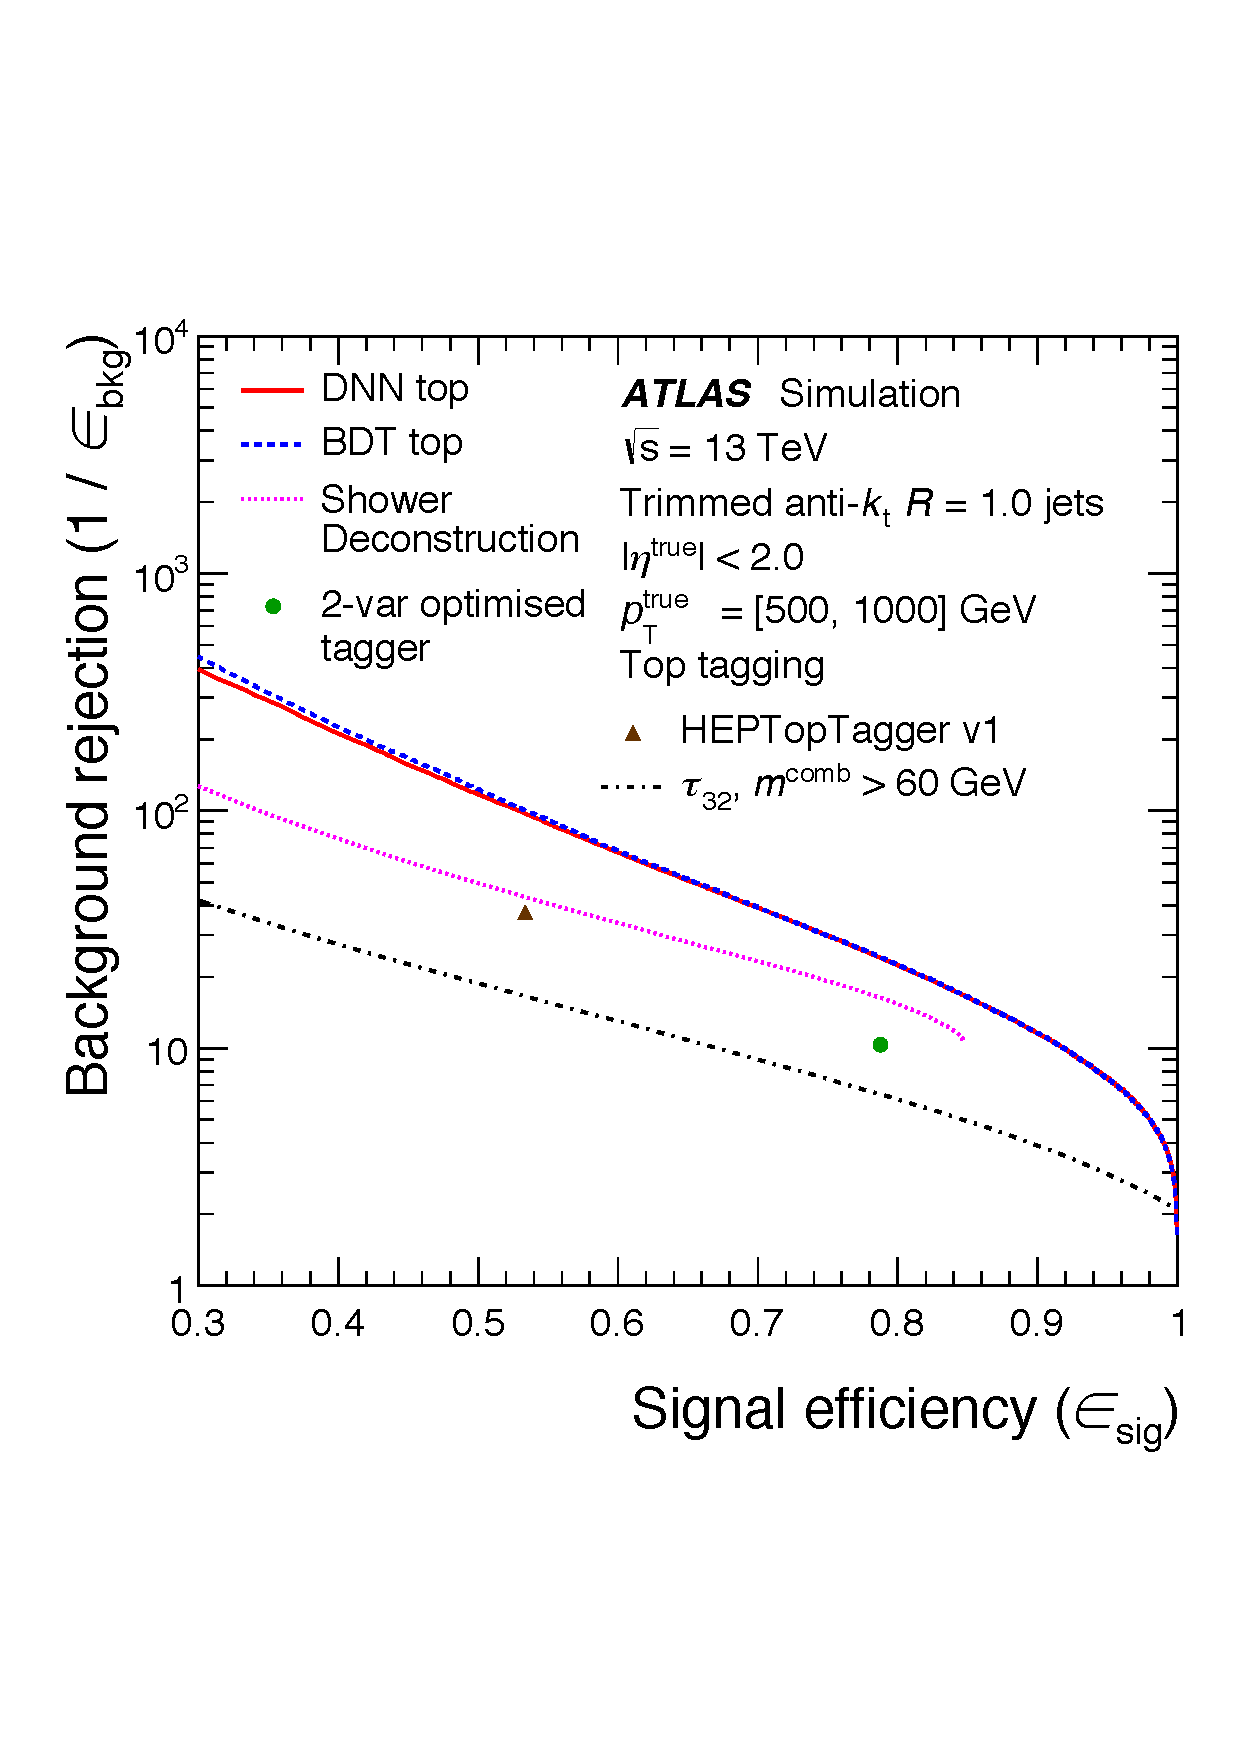
\includegraphics[width=0.485\textwidth]{figures/roc_topATLAS.pdf}
  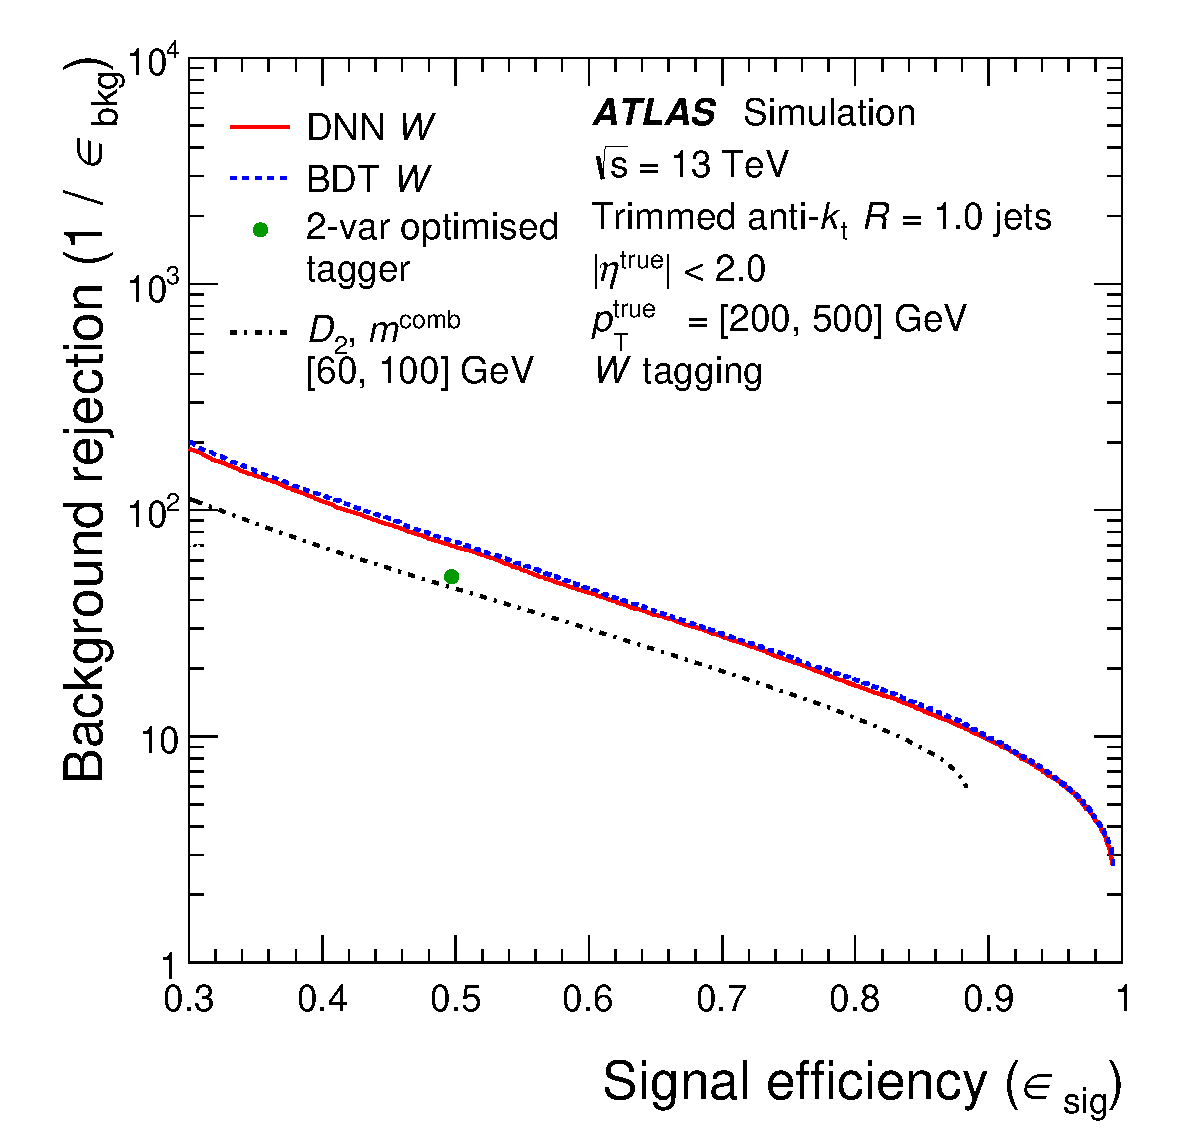
\includegraphics[width=0.515\textwidth]{figures/roc_WATLAS.pdf}
  \caption{Top quark (left) and W boson (right) tagging efficiencies for various tagging approaches used by ATLAS \cite{Aaboud:2018psm}.}\label{fig:roc_tag_atlas}
\end{figure}

CMS \cite{CMS:2016tvk, Khachatryan:2014vla} takes a similar approach
to W boson and top quark tagging as ATLAS. CMS uses a subset of the
observables of Table~\ref{tab:obs}, and extends it by including Qjet
volatility \cite{Ellis:2012sn} and $b$-tagging\footnote{For jets,
  $b$-tagging is meant to separate jets originating from a $b$ quark
  from light-quark and gluon jets. $b$-tagging algorithms are using
  the fact that $B$ hadrons decay with a displaced vertex together
  with a list of variables included in a BDT or neural network (with
  details depending on the experiment).} in their performance
analysis. In addition to the Shower Deconstruction tagger, an updated
version of the HEPTopTagger (V2) and the CMS top tagger are included
in the comparison. The results of Fig.~\ref{fig:roc_tag_cms} (left)
show that the performance of individual observables and taggers can
vary a lot, with Shower Deconstruction performing best in the signal
efficiency region of $\varepsilon_\mathrm{S} \leq 0.7$. However, when
various tagging methods are combined in a multivariate approach,
Fig.~\ref{fig:roc_tag_cms} (right), their performance become very
similar and the potential for further improvements seems to saturate
for the scenario at hand.
%
\begin{figure}
 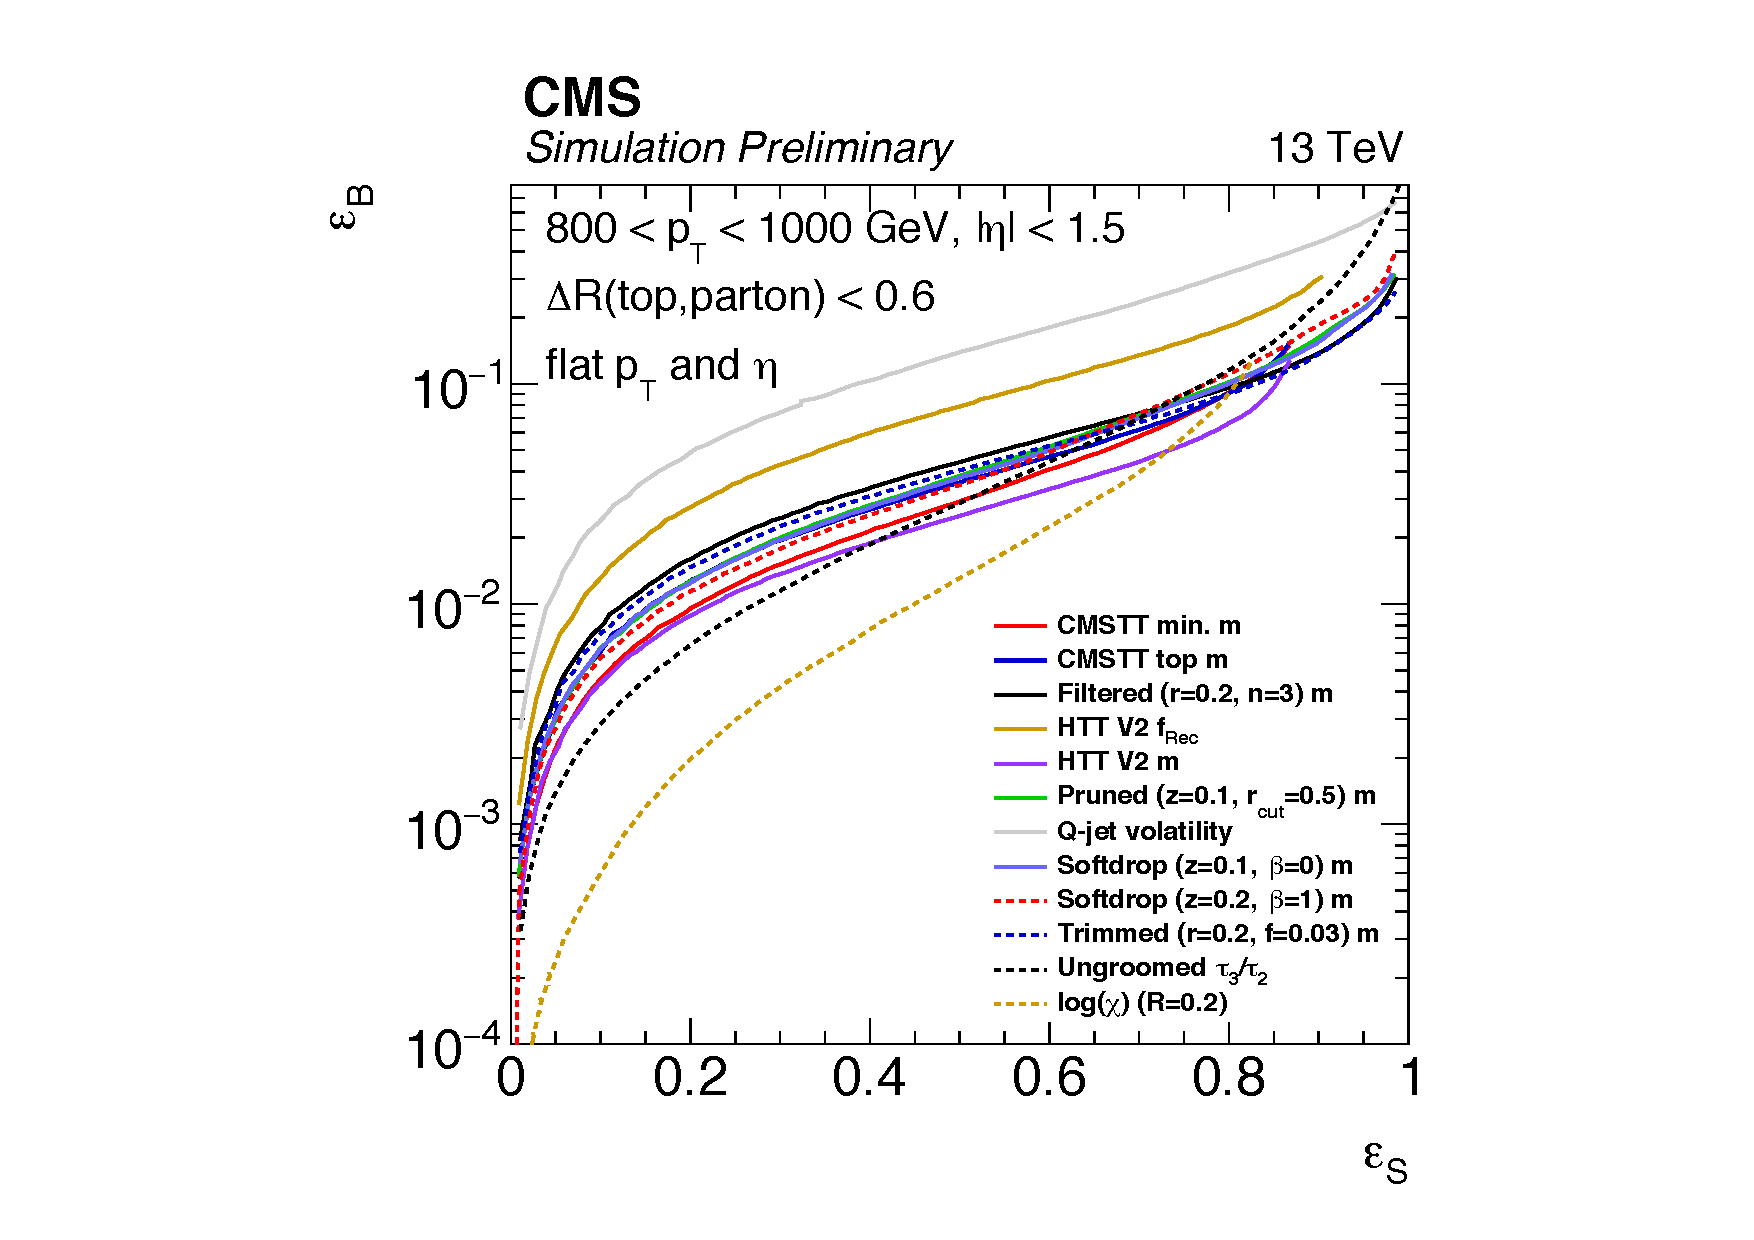
\includegraphics[width=0.5\textwidth]{figures/cms_top1_roc.pdf}
  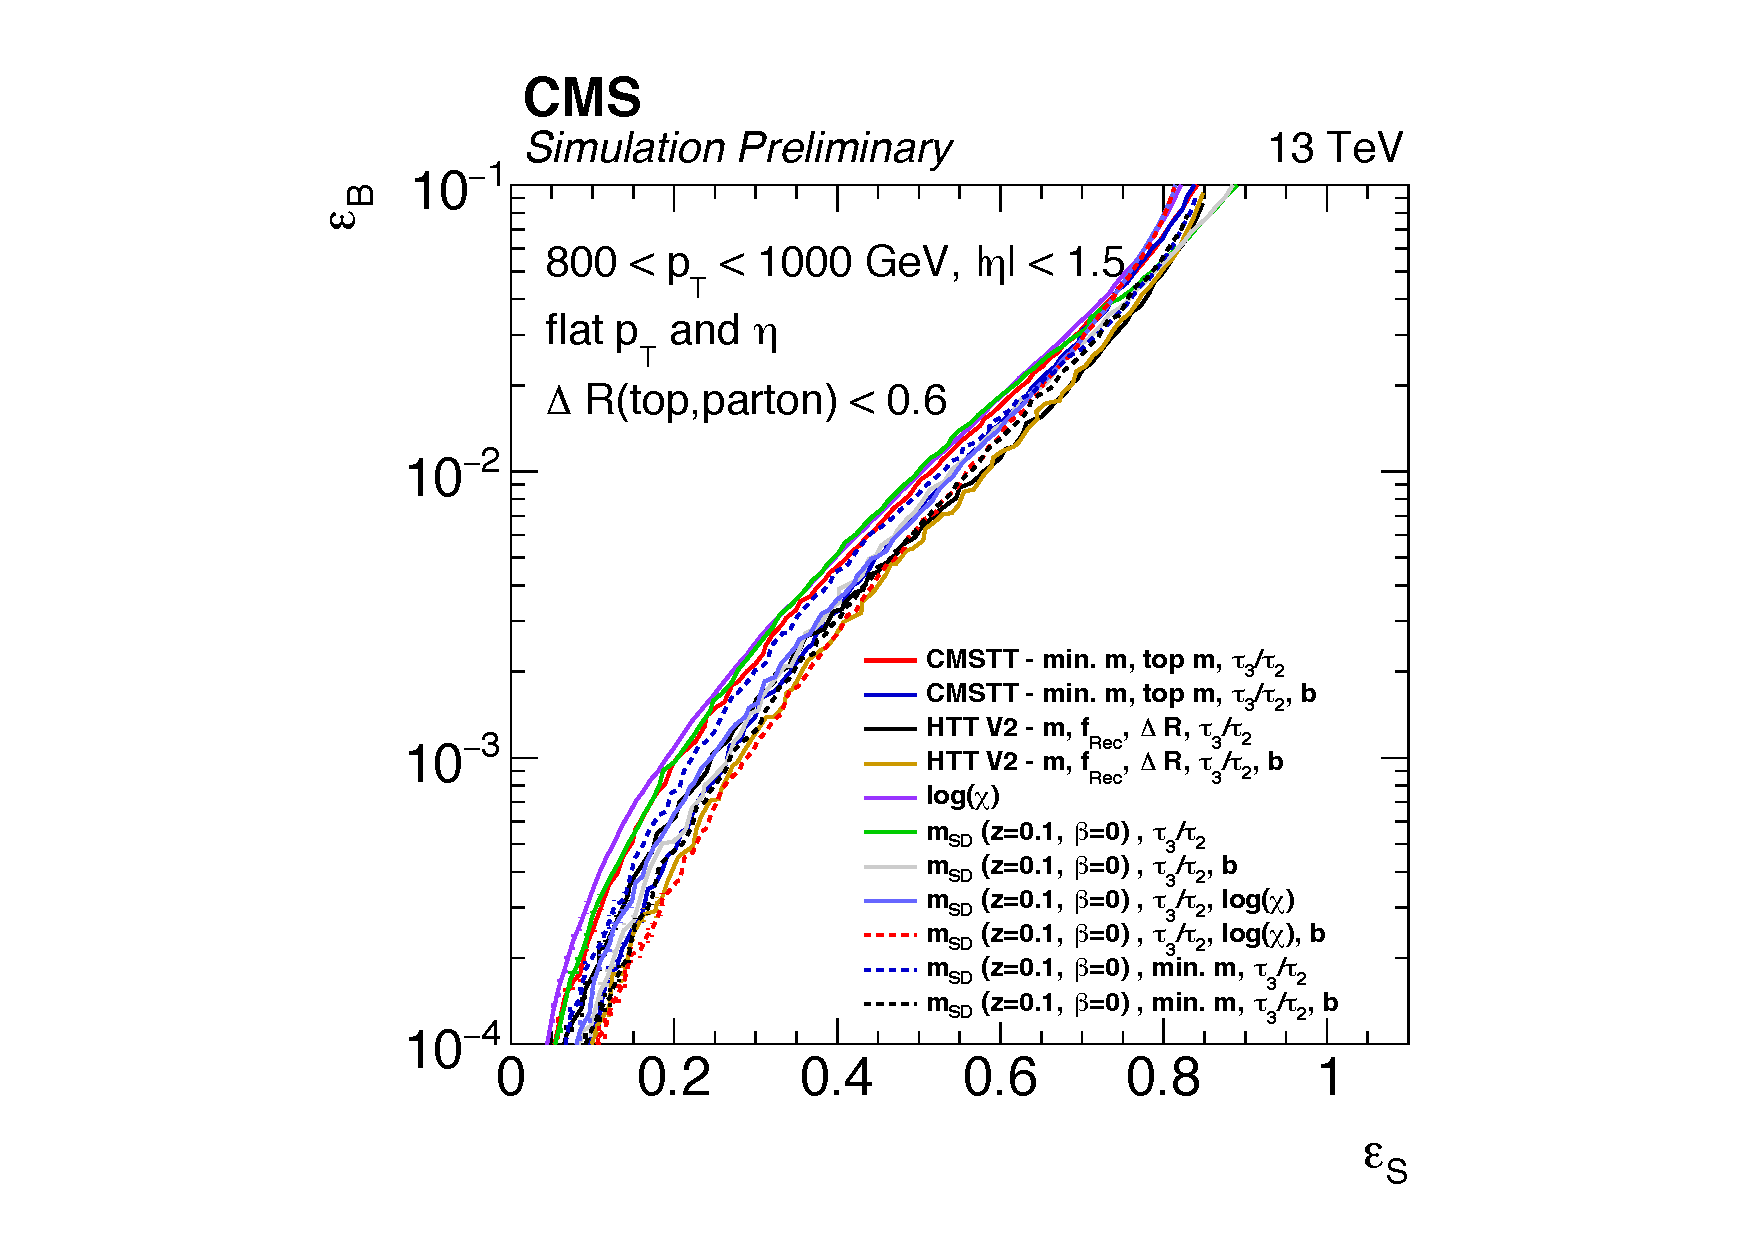
\includegraphics[width=0.5\textwidth]{figures/cms_top2_roc.pdf}
  \caption{Top quark tagging performance comparison from CMS \cite{CMS:2016tvk}.}\label{fig:roc_tag_cms}
\end{figure}
%
\begin{figure}
  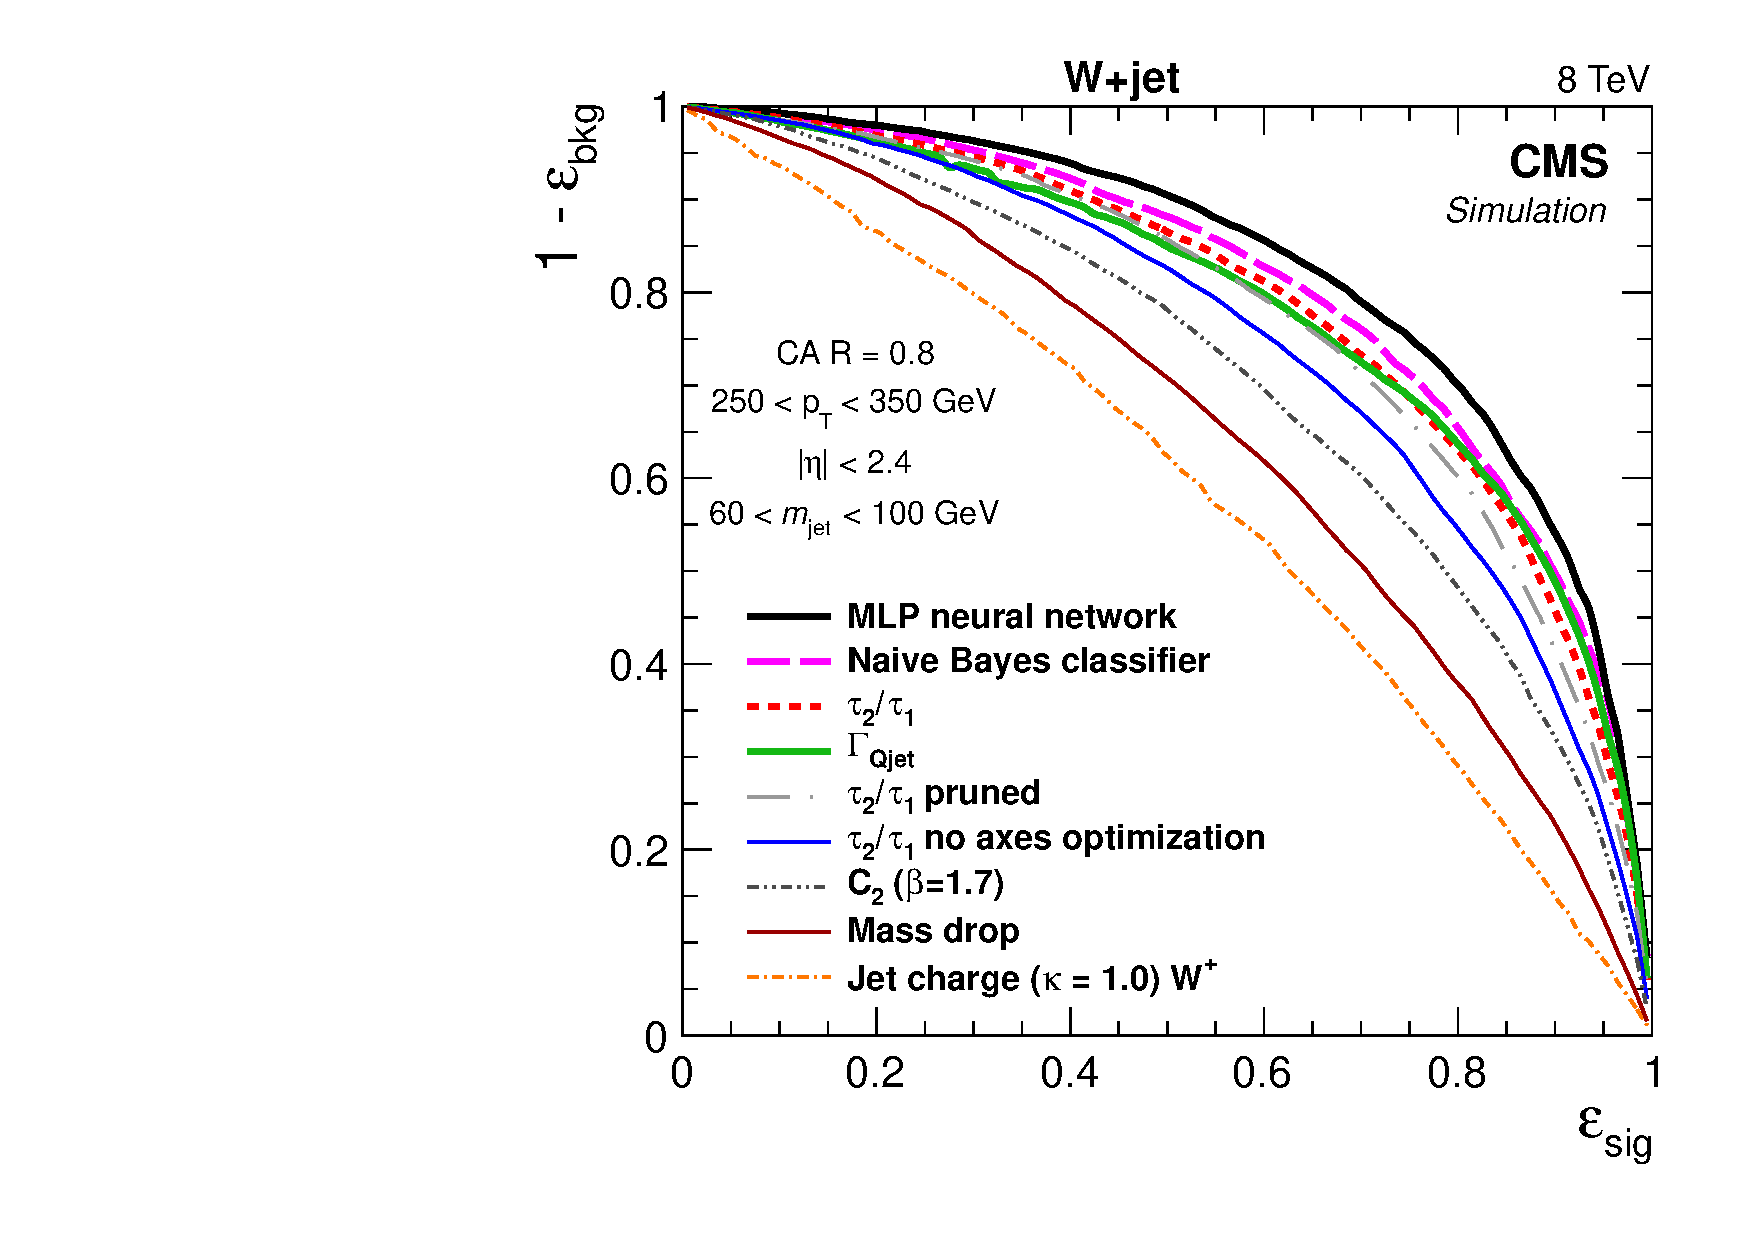
\includegraphics[width=0.5\textwidth]{figures/cms_W_roc.pdf}\hfill%
  \begin{minipage}[b]{0.42\textwidth}
    \caption{W boson tagging performance comparison from CMS~\cite{Khachatryan:2014vla}. 
  }\label{fig:cms_w_tag}
    \vspace*{2.4cm}
  \end{minipage}\hspace*{0.3cm}
\end{figure}
%
For W tagging, see Fig.~\ref{fig:cms_w_tag}, CMS combines several jet shape observables using either a naive Bayes classifier or a Multilayer Perceptron (MLP) neural network discriminant. When comparing to individual jet shape observables, such as $N$-subjettiness ratios or Qjet volatility, mild improvements can be achieved.  



The discrimination between quark and gluon-initiated jets can have profound phenomenological implications. A large class of processes associated with the production of new particles have a strong preference to result in quarks, e.g.\ the production and subsequent decay of squarks in the Minimal Supersymmetric Standard Model, while Standard Model QCD backgrounds are more likely to result in gluon-initiated jets. Thus, the ability to separate these two classes of jets reliably could boost our sensitivity in finding new physics. However, as discussed at length in Chapter~\ref{sec:calc-shapes-qg}, the discrimination between a jet that was initiated by a gluon from a jet that was initiated by a quark is subtle. 
%
Consequently, sophisticated observables which attempt to exploit small features between quarks and gluon jets can potentially be sensitive to limited experimental resolution and experimental uncertainties in the construction of the jet constituents.
%
In their performance studies, ATLAS~\cite{Aad:2014gea} and CMS~\cite{CMS:2017wyc} aim to exploit the differences in the radiation profiles between quarks and gluons using observables such as the number of charged tracks $n_{\mathrm{trk}}$, calorimeter $w_\mathrm{cal}$ or track width $w_\mathrm{trk}$ with
\begin{equation}
w = \frac{\sum_i p_{T,i} \times \Delta R\mathrm{(i,jet)}}{\sum_i p_{T,i}}\;,
\end{equation}
where $i$ runs either over the calorimeter energy clusters to form $w_\mathrm{cal}$ or over the charged tracks for $w_\mathrm{trk}$. Further observables are the track-based energy-energy-correlation (EEC) angularities
\begin{equation}
\mathrm{ang}_{\mathrm{EEC}} = \frac{\sum_i \sum_j p_{T,i} ~ p_{T,j} ~ (\Delta R(i,j))^\beta}{(\sum_i p_{T,i})^2}\;,
\end{equation}
where the index $i$ and $j$ run over the tracks associated with the jet, with $j>i$, and $\beta$ is a tunable parameter, the jet minor angular opening $\sigma_2$ of the $p_t^2$-weighted constituents distribution in the lego plane and the jet fragmentation distribution $p_{T}D$, defined as
\begin{equation}
p_{T}D = \frac{\sqrt{\sum_i p_{T,i}^2}}{\sum_i p_{T,i}},
\end{equation}
where $i$ runs over all jet constituents.
%
\begin{figure}[t]
  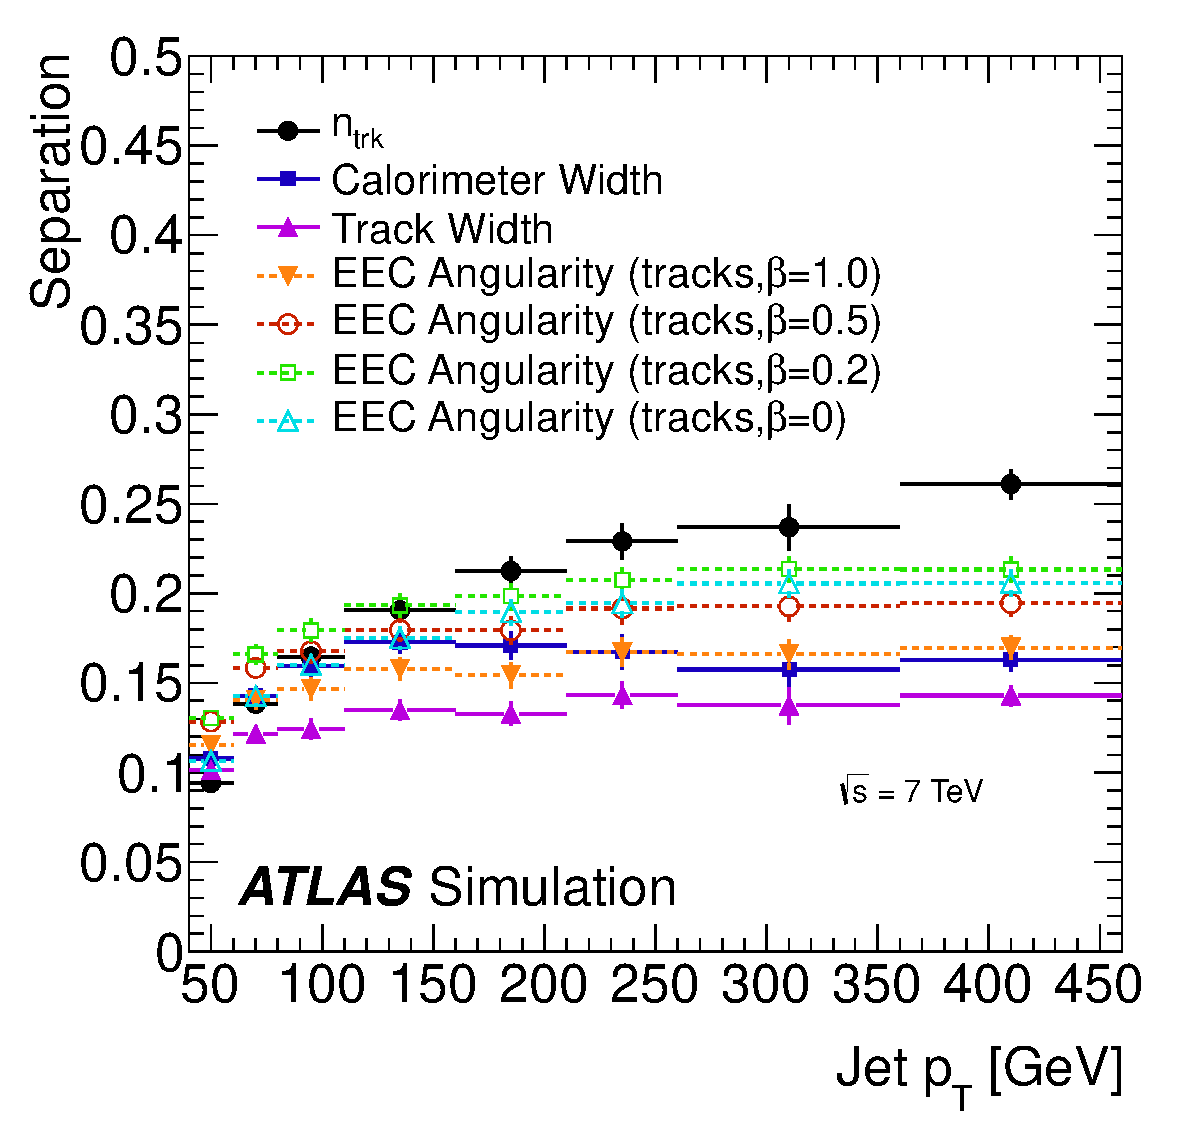
\includegraphics[width=0.47\textwidth]{figures/gq_atlas.pdf}
 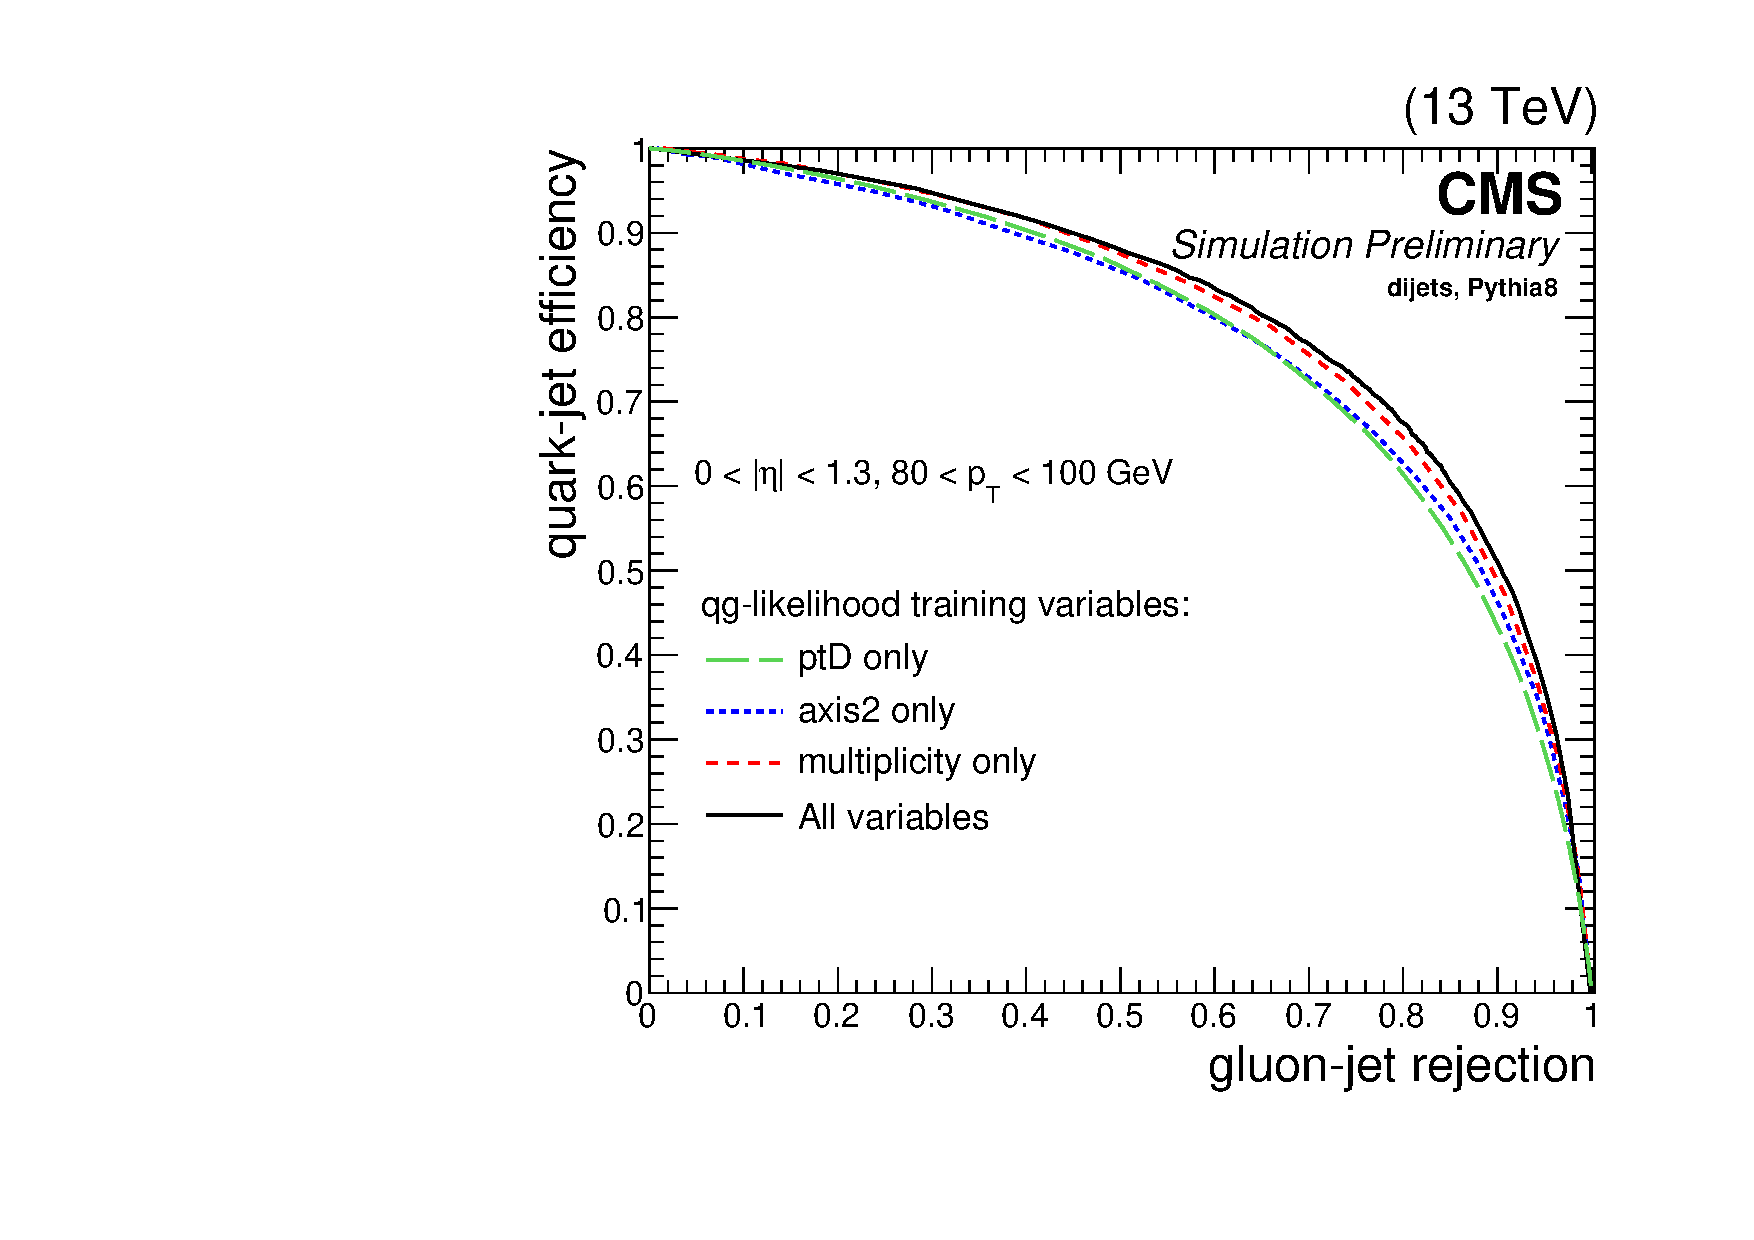
\includegraphics[width=0.51\textwidth]{figures/gq_cms.pdf}
  \caption{ATLAS (left) and CMS (right) studies of quark/gluon discrimination.
  The plots are taken from, respectively, Ref.~\cite{Aad:2014gea} and~\cite{CMS:2017wyc}. }\label{fig:exp_roc_qg}
\end{figure}

ATLAS results for quark-gluon tagging~\cite{Aad:2014gea, ATL-PHYS-PUB-2017-009} are reported in Fig.~\ref{fig:exp_roc_qg} on the left, in terms of the variable ``separation", which is defined as:
\begin{equation}
\mathrm{Separation} = \frac{1}{2} \int \frac{(p_q(x) - p_g(x))^2}{p_q(x) + p_g(x)} dx
\end{equation}
where $p_q(x)$ and $p_g(x)$ are normalised distributions of the variables used for discrimination between quark and gluon jets. 
%
Both experiments achieve a good separation between quark and gluon jets for the observables used and the $p_t$-windows studied. For example, CMS achieves for a $50\%$ quark jet acceptance a rejection of roughly $90\%$ of gluon jets.



\section{Measurements of jet observables}
\begin{figure}[t!]
 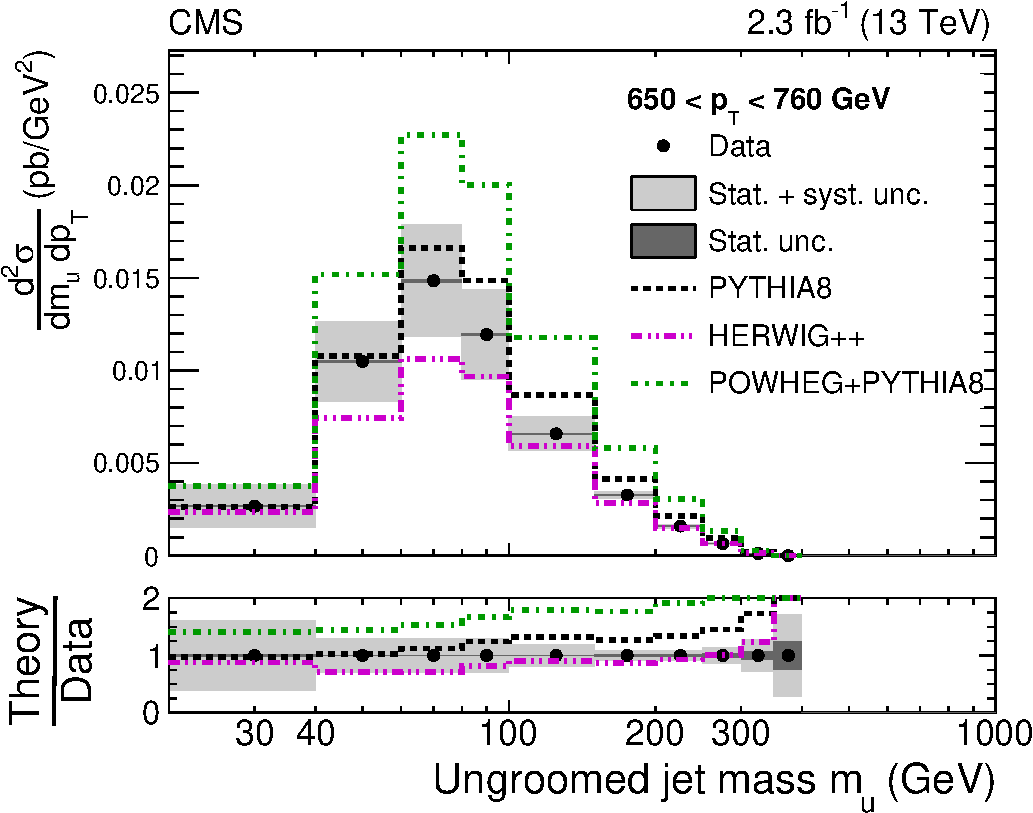
\includegraphics[width=0.5\textwidth]{figures/CMS_jetmass_ungroomed.pdf} 
 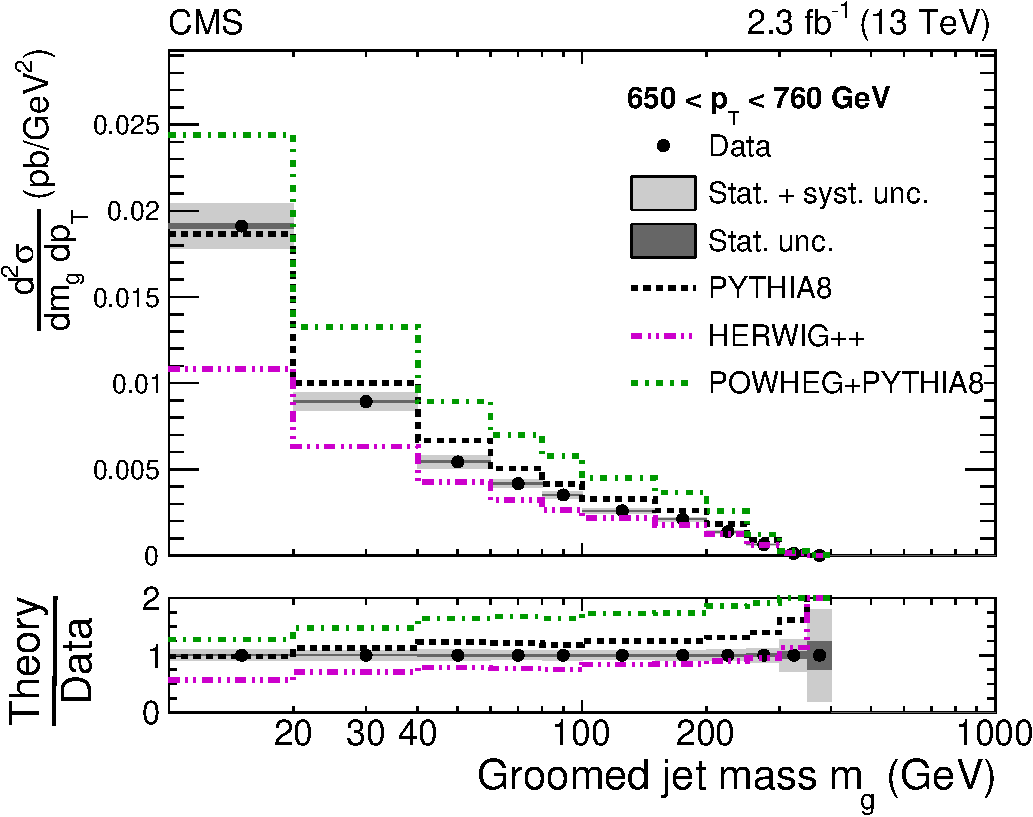
\includegraphics[width=0.5\textwidth]{figures/CMS_SD_jetmass_total.pdf} \\
 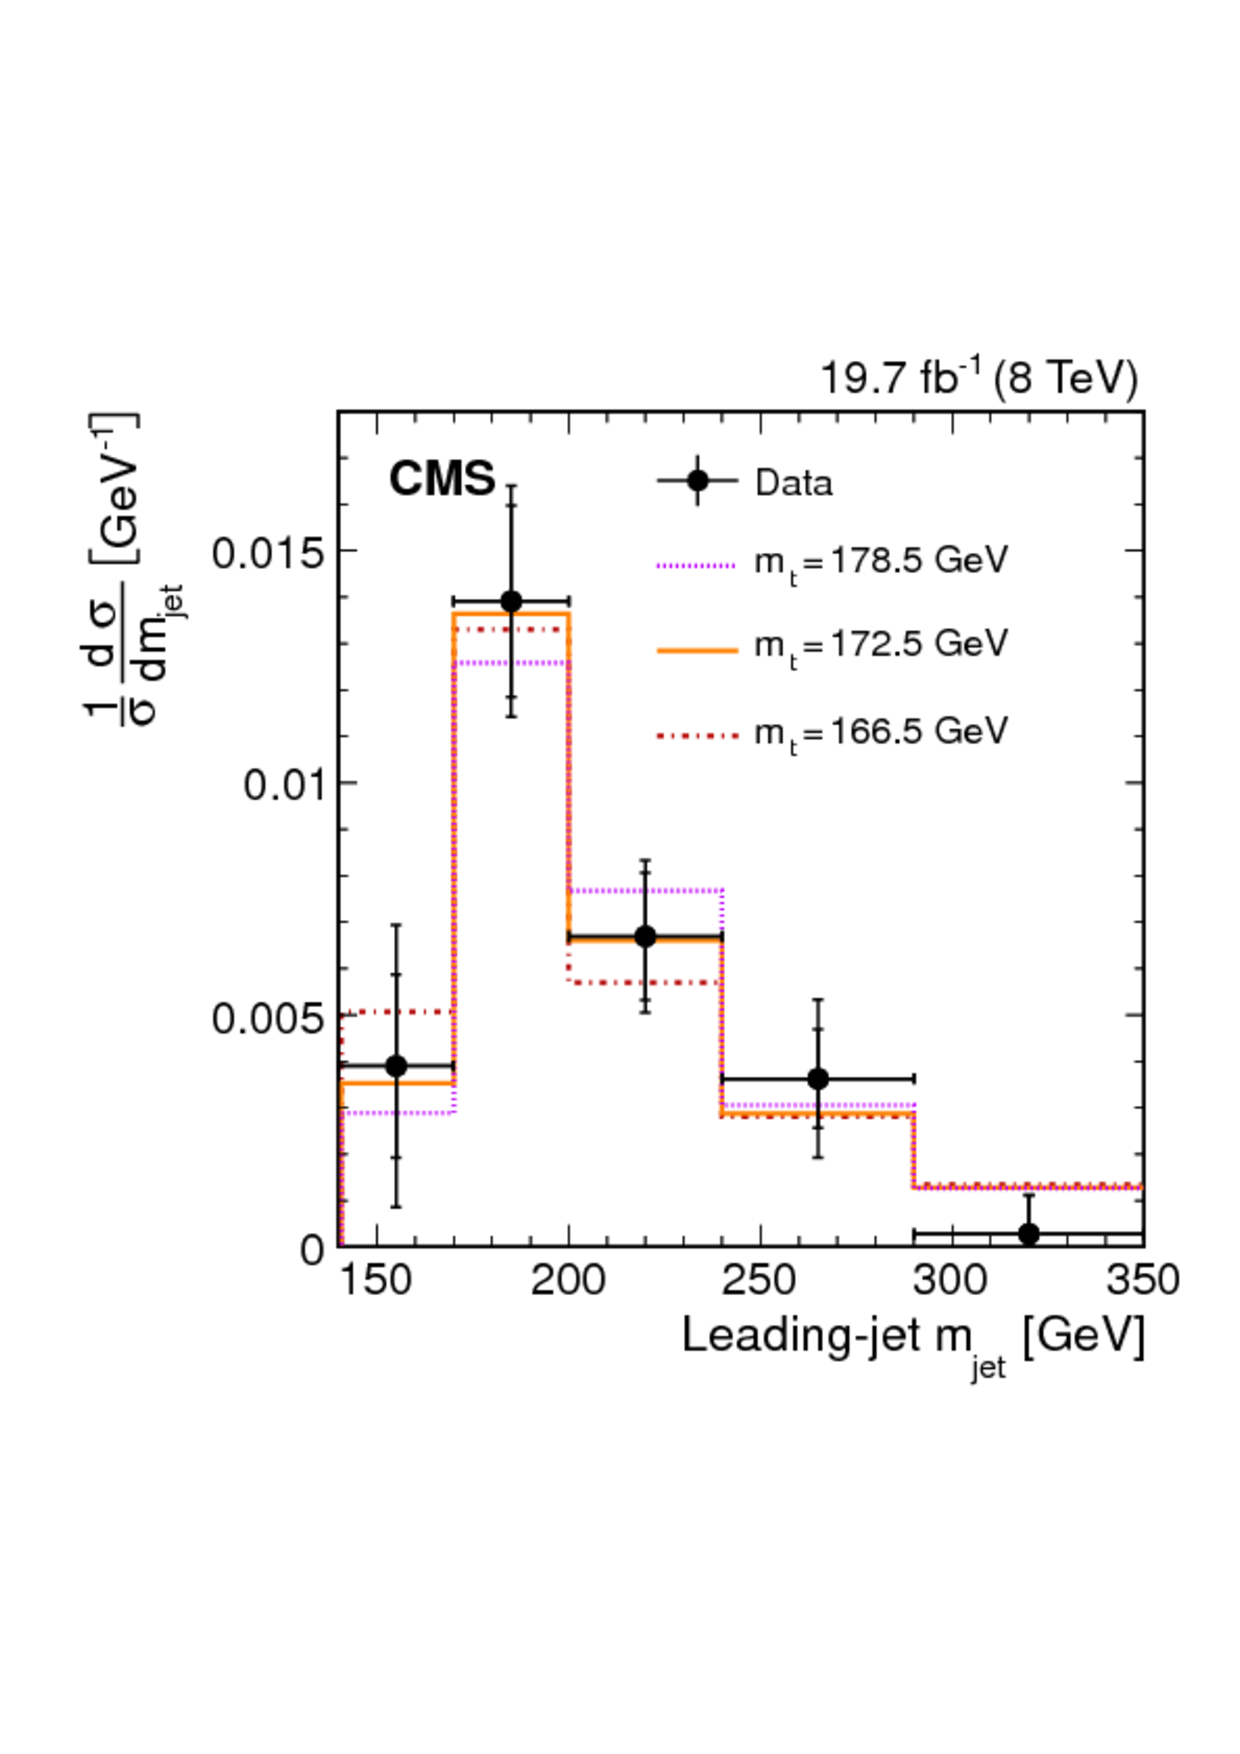
\includegraphics[width=0.45\textwidth]{figures/CMS_jetmass_top.pdf} 
 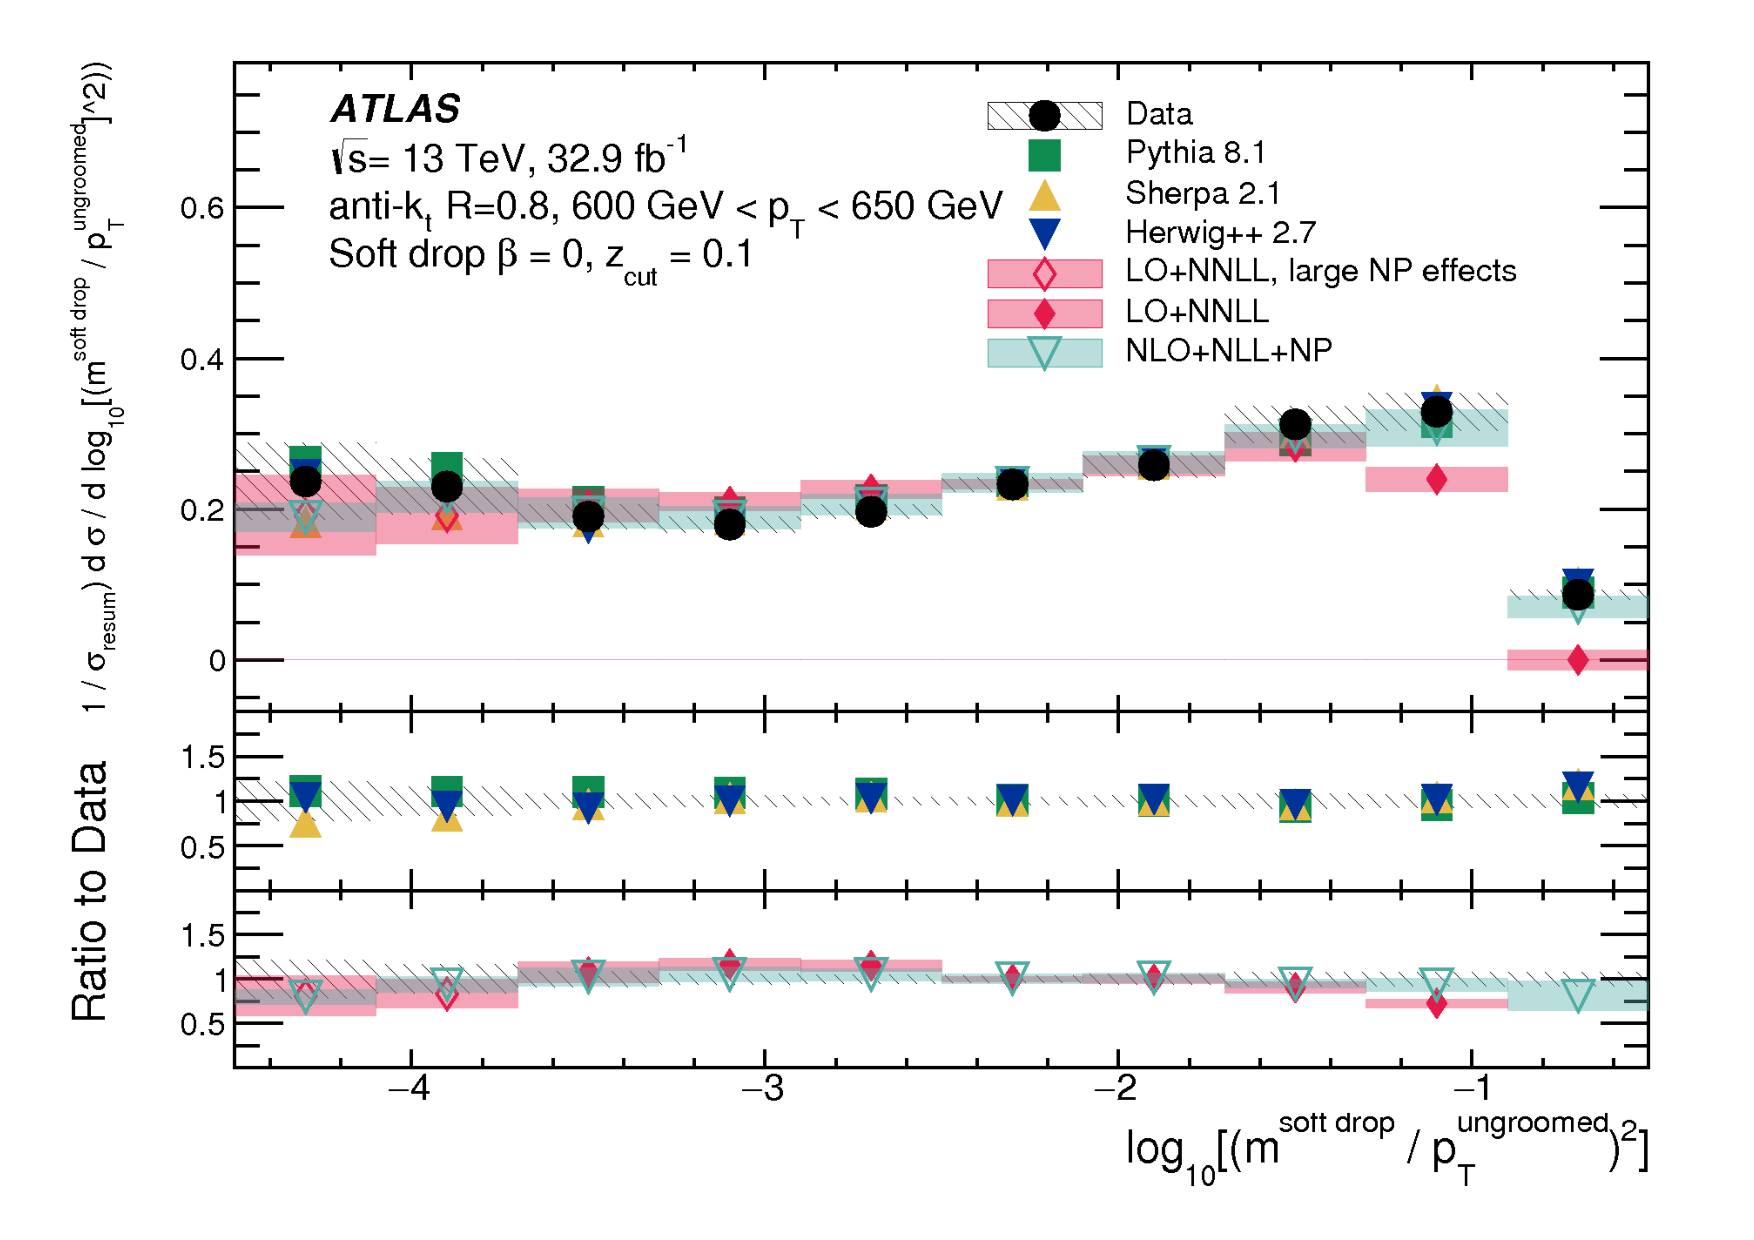
\includegraphics[width=0.55\textwidth]{figures/ATLAS_SD_jetmass.pdf}
  \caption{Jet mass measurements at the LHC, starting from the top
    left and going clockwise, we have: plain jet mass by CMS
    \cite{Sirunyan:2018xdh}, \SD (mMDT) jet mass by CMS \cite{Sirunyan:2018xdh}, \SD mass measurement by
    ATLAS~\cite{Aaboud:2017qwh}, and top jet mass by CMS \cite{Sirunyan:2017yar}.}\label{fig:jet_mass}
\end{figure}


Various jet observables discussed in Chapters~\ref{tools}-\ref{sec:curiosities} have been measured by ATLAS and CMS. In the following we will discuss a selection of the measurements performed for these observables and we will focus on measurements for large-$R$ jets.

\subsection{Jet mass}\label{sec:exp-jet-mass}

The mass of a jet is one of the most basic observables associated with a jet. As such, it was discussed in great detail in Chapters~\ref{chap:calculations-jets} and \ref{calculations-substructure-mass}, with and without the application of various grooming methods to the jet. As the mass is sensitive to the energy distribution in the jet, it can also be thought of as a jet-shape observable.

ATLAS \cite{ATLAS:2012am, Aaboud:2017qwh} and CMS~\cite{Sirunyan:2017yar, Sirunyan:2018xdh} have both measured the mass of jets under various conditions. In \cite{ATLAS:2012am} ATLAS has measured the jet mass, amongst other jet shape and jet substructure observables, in $pp$ collisions at a centre-of-mass energy of 7~TeV. 

The \SD mass has been measured in \cite{Aaboud:2017qwh} and \cite{
  Sirunyan:2018xdh} by ATLAS and CMS, respectively. After requiring a
jet with $p_t > 600$ GeV and imposing the dijet topology cut
$p_{T,1}/p_{T,2} < 1.5$, ATLAS runs the soft-drop algorithm on the two
leading jets in the events. Three different values of $\beta \in
{0,1,2}$ are considered, while the value on the $z_\mathrm{cut}$ is
fixed at $0.1$. Then the dimensionless ratio $m^{\mathrm{soft~drop}}/p_t^{\mathrm{ungroomed}}$ is constructed and
shown in Fig~\ref{fig:jet_mass} in the lower right panel. The measured data is in good agreement with various theoretical predictions, including resummed analytic calculations and full event generators.
%
CMS selects similar event kinematics for this measurement, but fixes $\beta=0$. In Fig.~\ref{fig:jet_mass} in the upper right and upper left panel the groomed and ungroomed jet mass, measured by CMS at 13 TeV centre-of-mass energy, is shown respectively. Data is compared with theory predictions from Pythia8, Herwig++ and Powheg+Pythia8, showing significant differences between the three event generators. While the overall normalisation of the cross sections predicted by the event generators is quite different, with Pythia8 being closest to data, the shape of the theoretically predicted distributions agree well with data. Thus, when the distributions are normalised to the total cross section, the difference between data and all three theory predictions is small.

The precision with which a boosted top quark's mass can be measured by analysing a fat jet is a crucial parameter for many tagging algorithms. In \cite{Sirunyan:2017yar} CMS purifies the final state with respect to semi-leptonic $t\bar{t}$ events and reconstructs Cambridge/Aachen $R=1.2$ fat jets with $p_t>400$ GeV. The mass of the leading fat jet is sown in the lower left panel of Fig.~\ref{fig:jet_mass}. No special grooming procedure has been used, yet the measured jet mass agrees well with the physical top mass. 



\begin{figure}[t]
  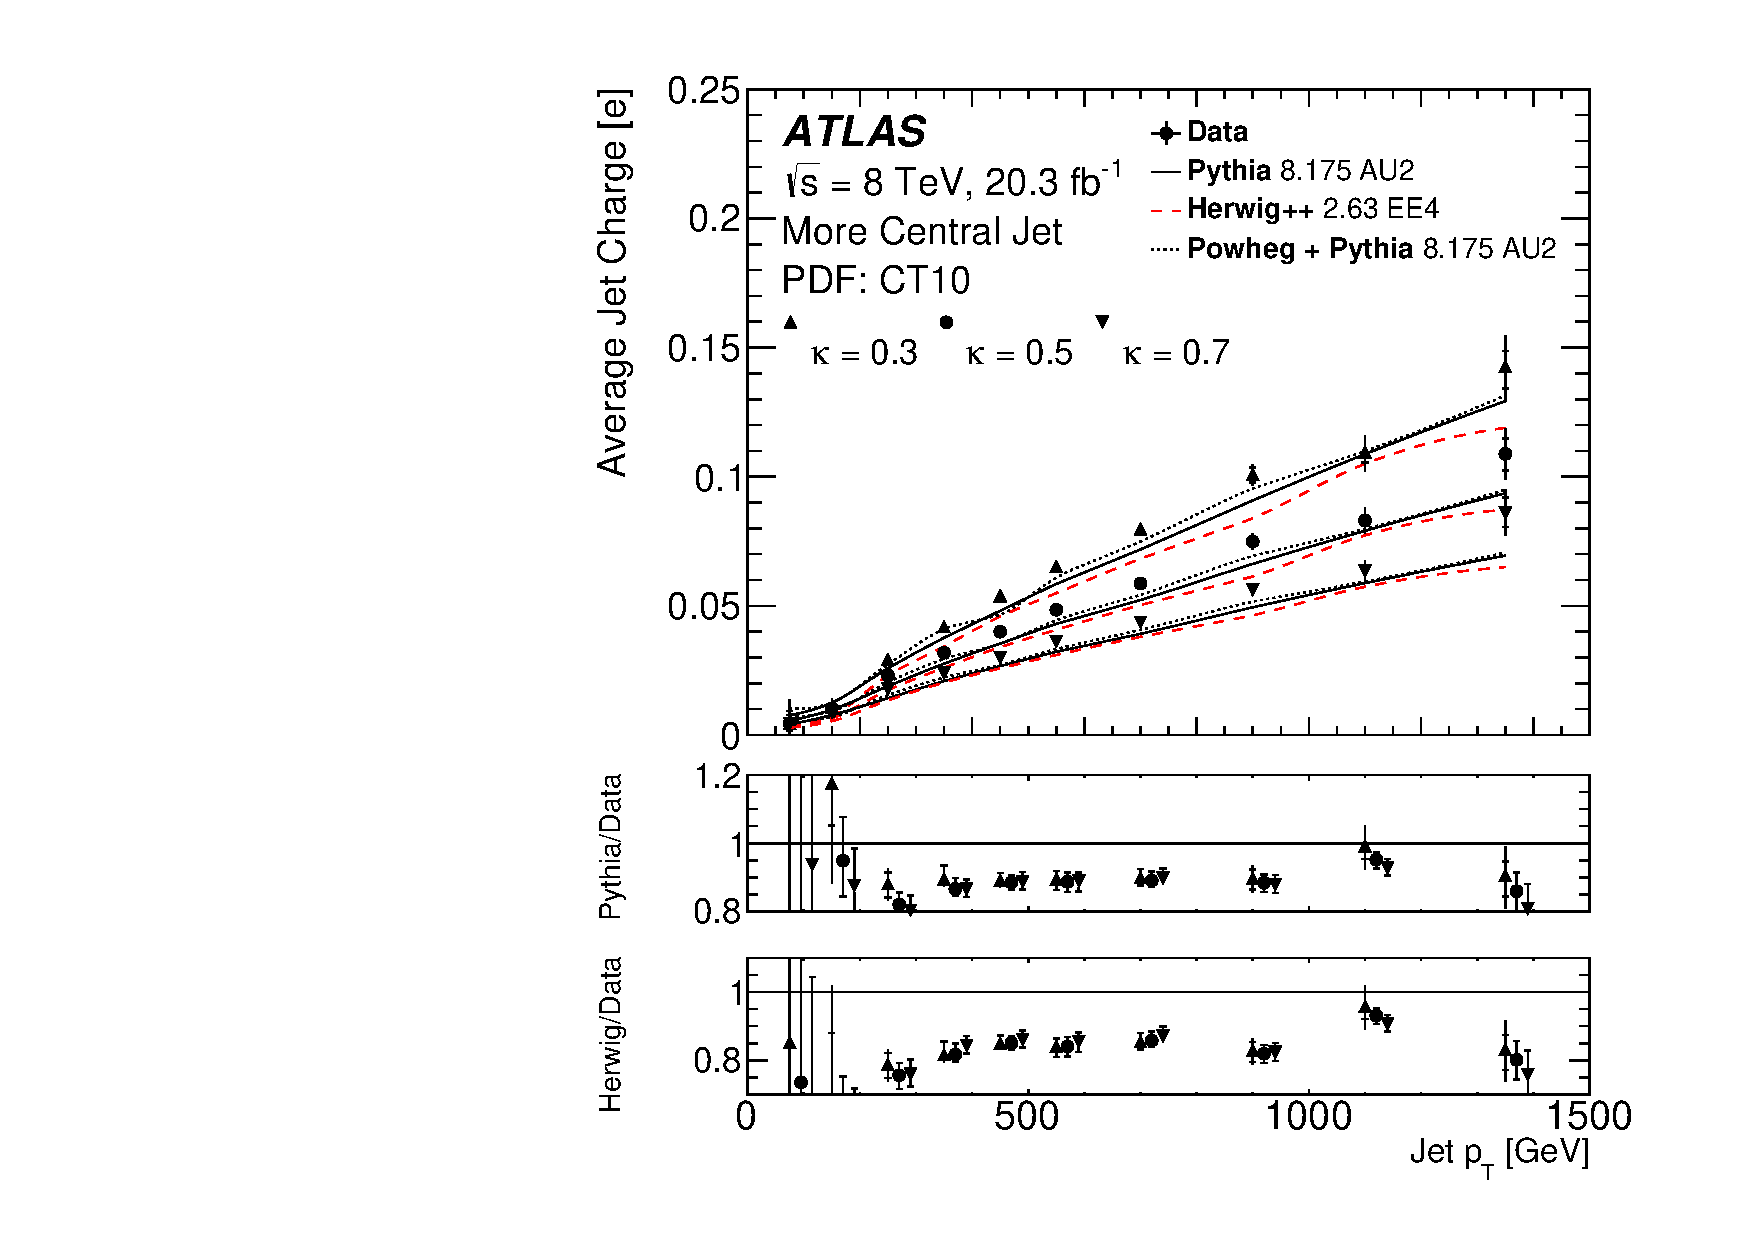
\includegraphics[width=0.45\textwidth]{figures/charge_ATLAS.pdf}
 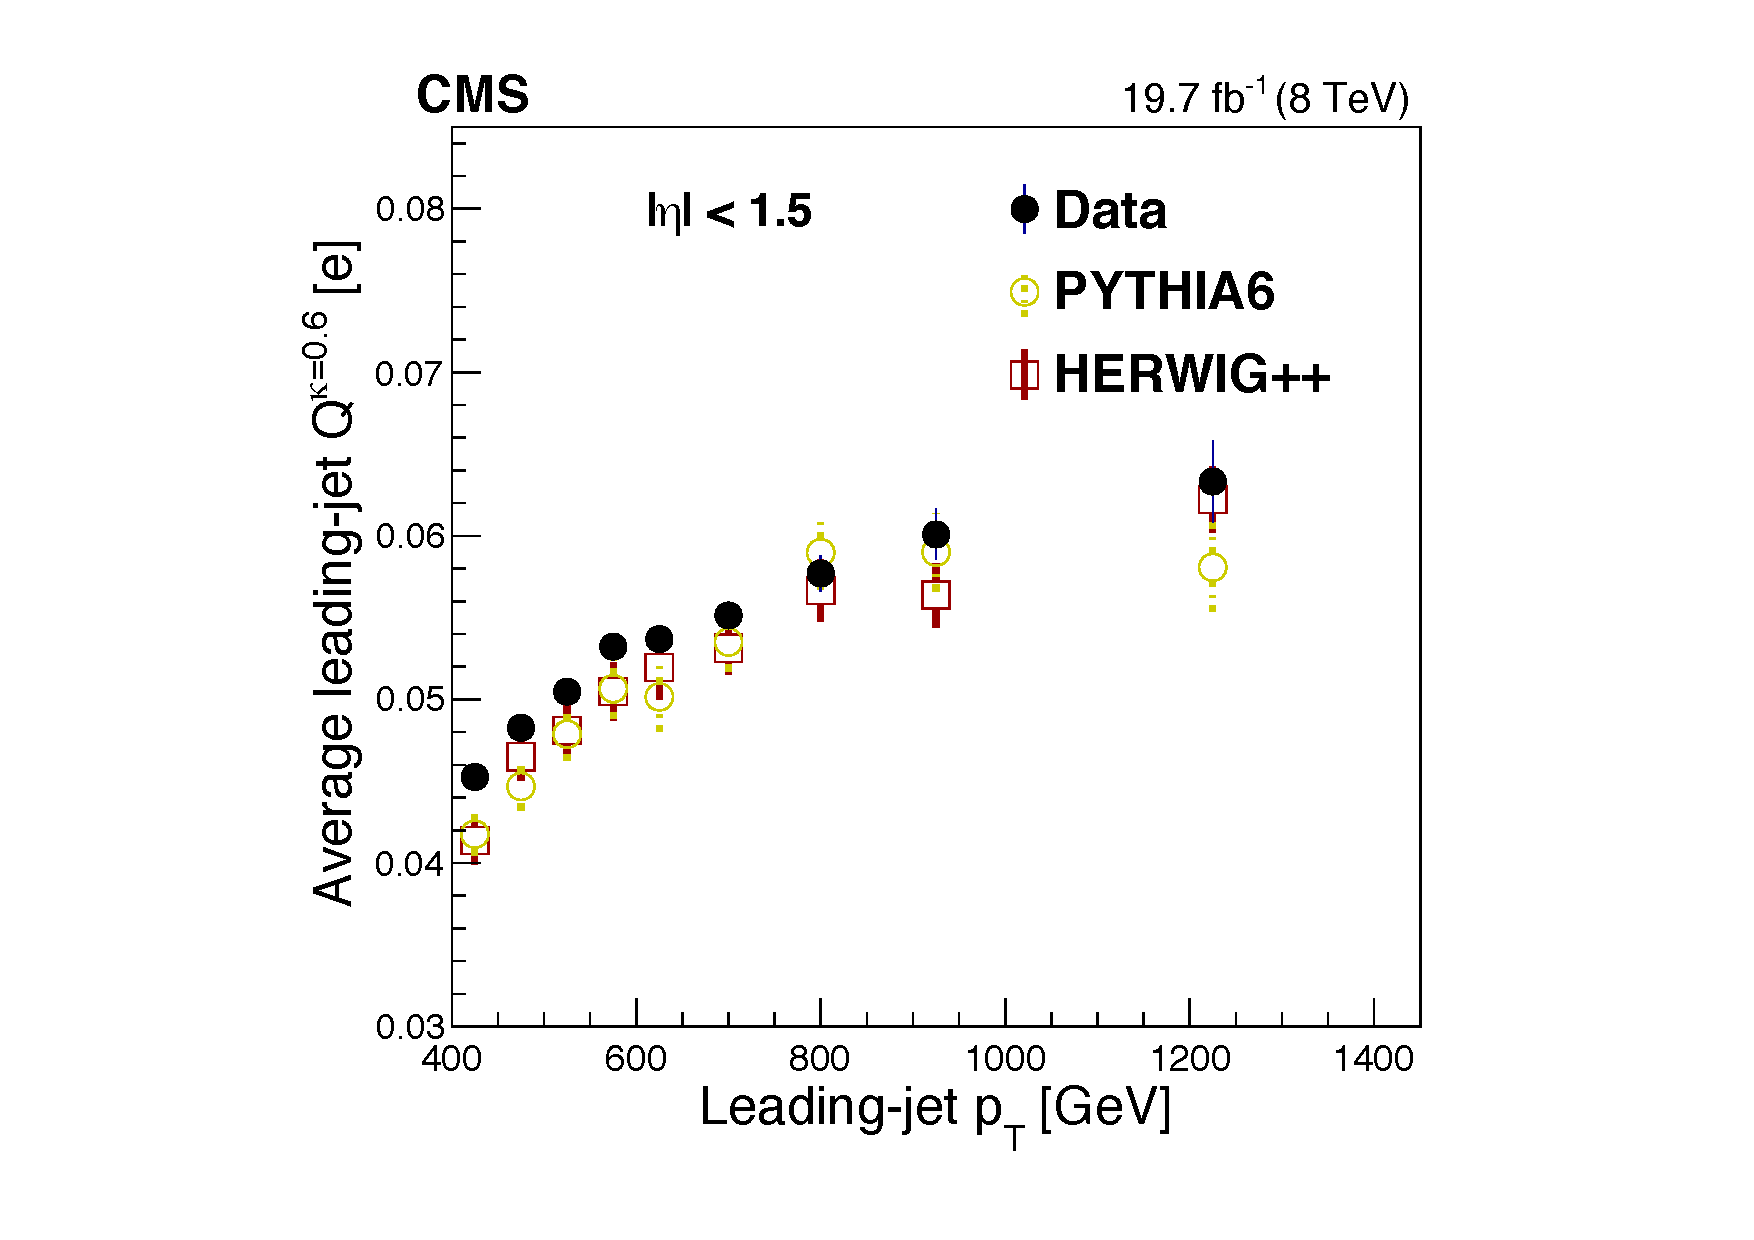
\includegraphics[width=0.65\textwidth]{figures/charge_CMS.pdf}
  \caption{Measurements of the jet charge by ATLAS~\cite{Aad:2015cua} (left) and CMS~\cite{Sirunyan:2017tyr} (right).}\label{fig:exp_charge}
\end{figure}

\subsection{Jet charge}

The energy deposits and tracks associated with a jet can originate from dozens of charged particles, depending on the size and on transverse momentum of the jet. If charged particles become too soft, e.g. $p_t \ll 1$ GeV, they can curl up in the magnetic field of the detector and might not even be measurable in the calorimetry or the tracker. Thus, it is useful to define the jet charge as a $p_t$-weighted sum of the charge of the jet constituents.
As the number of charged particles amongst the jet constituents is neither an infrared-safe nor a perturbatively calculable quantity, experimental measurements of these observables have to be compared to fitted hadronisation models included in full event generators.
%
A natural and common definition for the jet charge is  \cite{Aad:2015cua,Sirunyan:2017tyr} 
\begin{equation}
Q_J = \frac{1}{(p_{T,J})^\kappa} \sum_{i \in \mathrm{tracks}} q_i ~(p_{T,i})^\kappa \;,
\end{equation}
where $i$ runs over all tracks associated with jet $J$. $q_i$ is the
measured charge of track $i$ with associated transverse momentum
$p_{T,i}$, and $\kappa$ is a free regularisation
parameter.\footnote{There are alternative definitions of jet
  charge. For examples and how their theoretical prediction compares
  to experimental measurements, see~\cite{Sirunyan:2017tyr}.} In this
definition the charge associated with individual tracks, \ie
individual charged particles, is weighted by their transverse
momentum.
%
That way $Q_J$ is less sensitive to experimental and theoretical uncertainties. 
ATLAS and CMS both find good agreement between theoretical predictions and data over a large range of transverse momenta of the jets, when calculating their average charge, see Fig.~\ref{fig:exp_charge}. 



\subsection{Splitting functions}

\begin{figure}[t]
  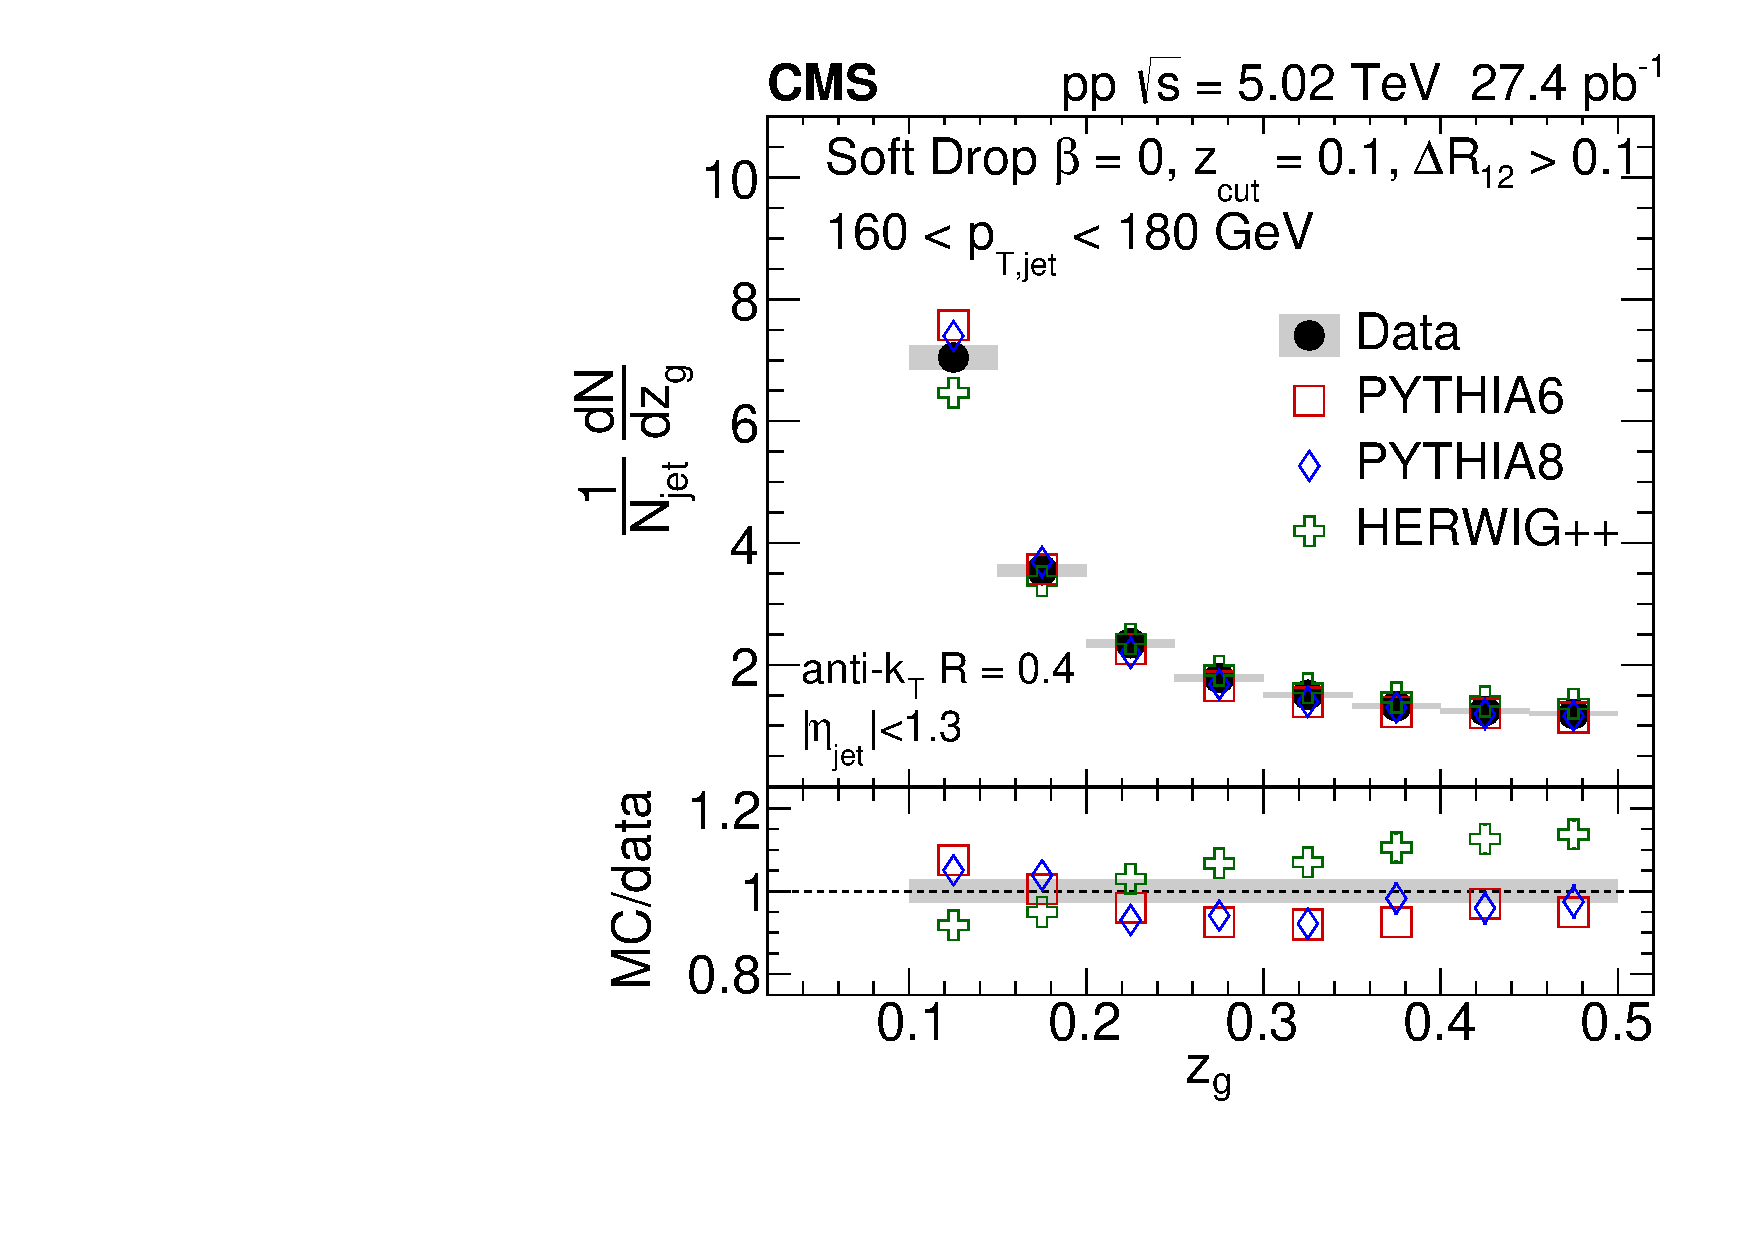
\includegraphics[width=0.5\textwidth]{figures/splitting_cms.pdf}\hfill%
  \begin{minipage}[b]{0.42\textwidth}
    \caption{The groomed momentum sharing $z_g$ measured by CMS during LHC's heavy-ion runs in $pp$ collisions \cite{Sirunyan:2017bsd}.}
    \label{fig:exp_splitting}
    \vspace*{1.4cm}
  \end{minipage}\hspace*{0.3cm}
\end{figure}

The momentum sharing $z_g$ between the two subjets that pass the \SD condition was introduced in Sec.~\ref{sec:zg}. The variable $z_g$ can be taken as a proxy of the "most important" partonic splitting in the jet evolution and thus its distribution is governed by the QCD splitting functions.
%
A measurement\footnote{Note that we refer here to observables that have not been unfolded. Thus, a comparison of data to theoretical predictions requires the knowledge of detector effects on the reconstructed observable.} of the $z_g$ distribution in $pp$ collisions, using CMS open data, was reported in \cite{Larkoski:2017bvj, Tripathee:2017ybi}. 
%
Using data obtained during LHC's heavy-ion runs, CMS has studied $z_g$ in PbPb and $pp$ collisions \cite{Sirunyan:2017bsd}. A measurement in of $z_g$ in PbPb collisions reflects how the two colour-charged partons produced in the first splitting propagate through the quark-gluon plasma, thereby probing the role of colour coherence of the jet in the medium. In the $pp$ case all particle-flow anti-$k_t$ jets with $R=0.4$ and $p_{t,j} > 80$ GeV were recorded. To identify the hard prongs of a jet and to remove soft wide-angle radiation, \SD grooming is applied to the jets with $\beta=0$ and $z_\mathrm{cut}=0.1$. 
%
Fig.~\ref{fig:exp_splitting} shows the comparison of $z_g$ between the measured CMS data and the theoretical predictions from Pythia6, Pythia8 and Herwig++, including a full simulation of detector effects. While in general good agreement is observed, both Pythia simulations have a slightly steeper $z_g$ distribution than the data, whereas Herwig++ shows an opposite trend.


\section{Search for boosted Higgs boson in the SM}

The possibility to search for the Standard Model Higgs boson in the decay to $b\bar{b}$ at the LHC using jet substructure techniques gave the field of jet physics a tremendous boost \cite{Butterworth:2008iy}. The projected sensitivity for a discovery of the Higgs boson with only $\sim 30~\mathrm{fb}^{-1}$, however, requires a centre-of-mass energy of 14 TeV for LHC proton-proton collisions. Due to technical issues of the LHC to reach its design energy of 14 TeV during Runs I and~II, the decay of a Higgs boson into a $b\bar{b}$-pair was never a contender to contribute to its discovery. Still, the measurement of the Higgs boson coupling to bottom quarks, while notoriously difficult, is of crucial importance as it is a dominant contributor to the total width of the Higgs boson, which in turn affects the branching ratios of all available decay modes. 

\begin{figure}
  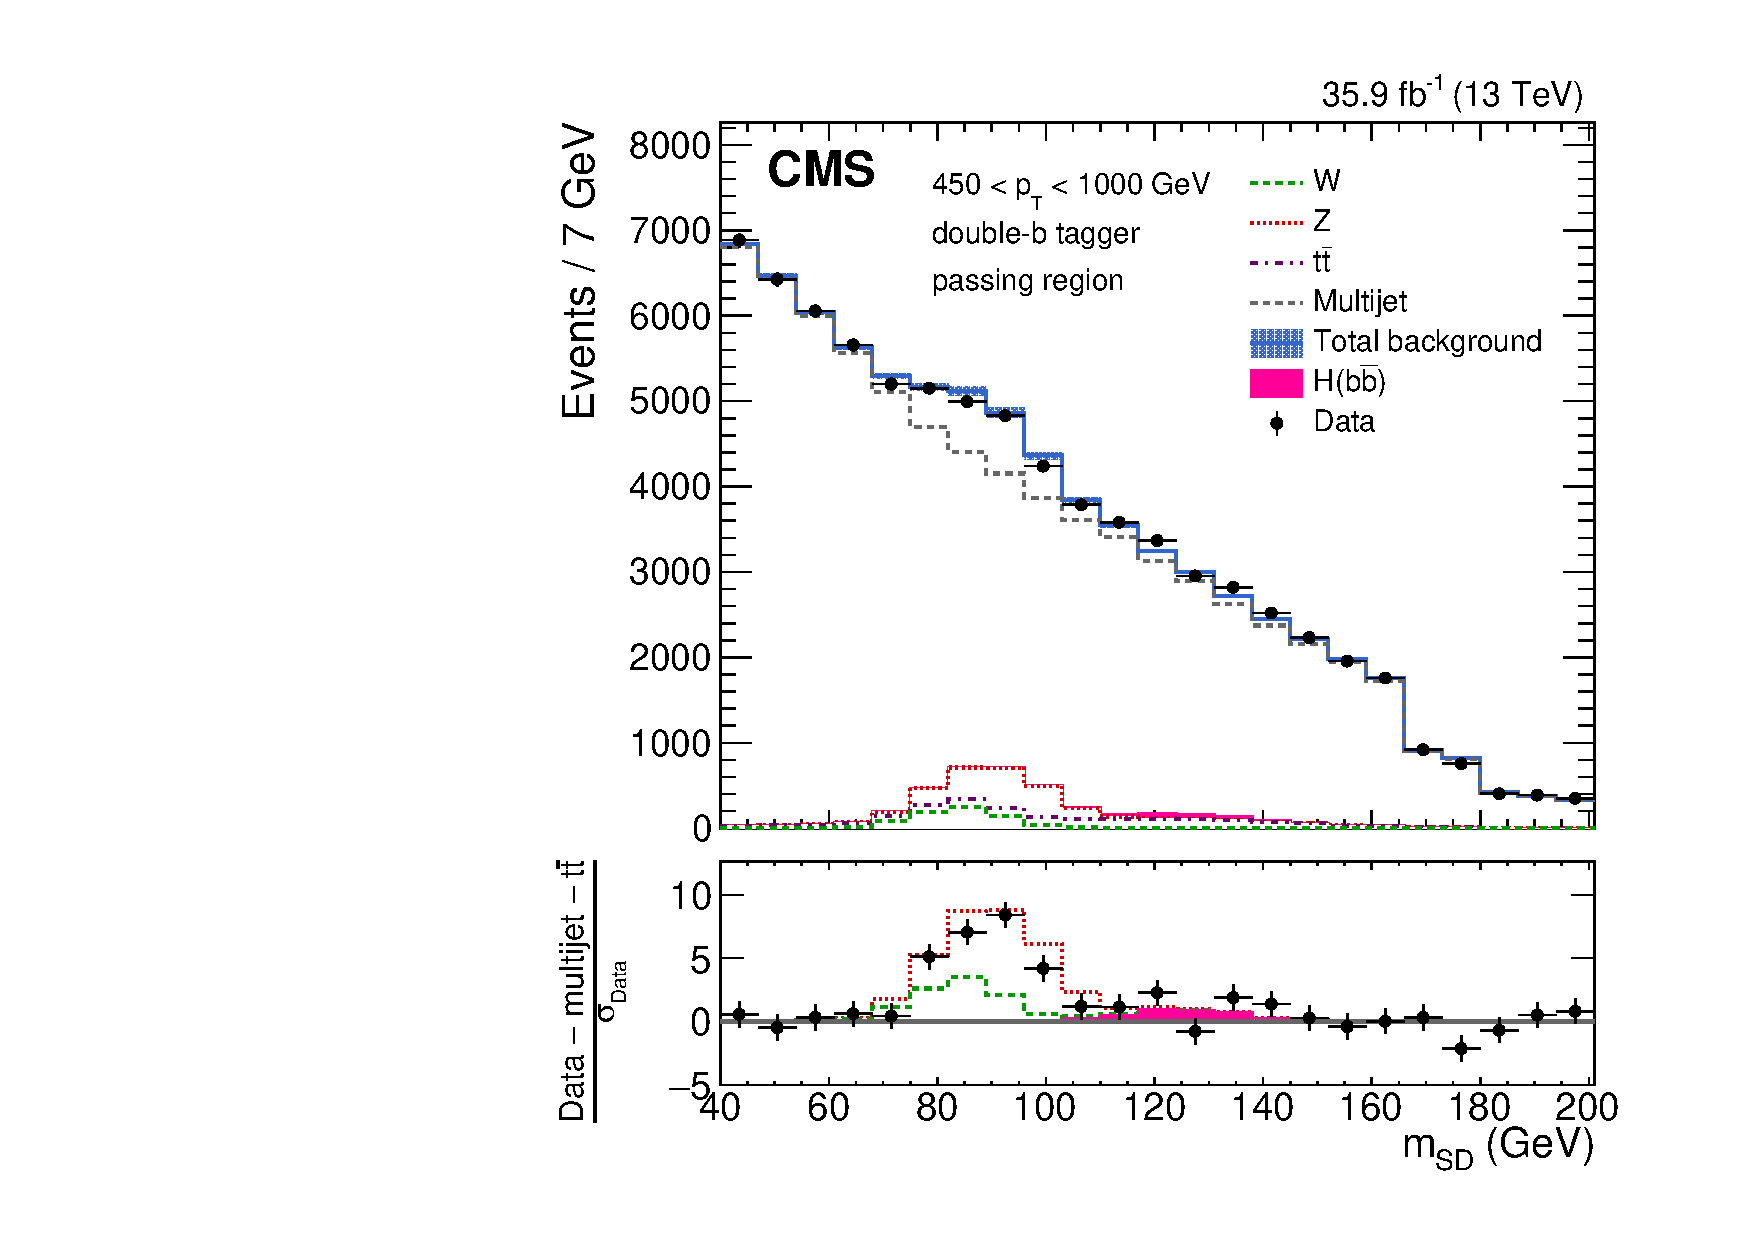
\includegraphics[width=0.45\textwidth]{figures/cms_SM_boostedH.pdf}
    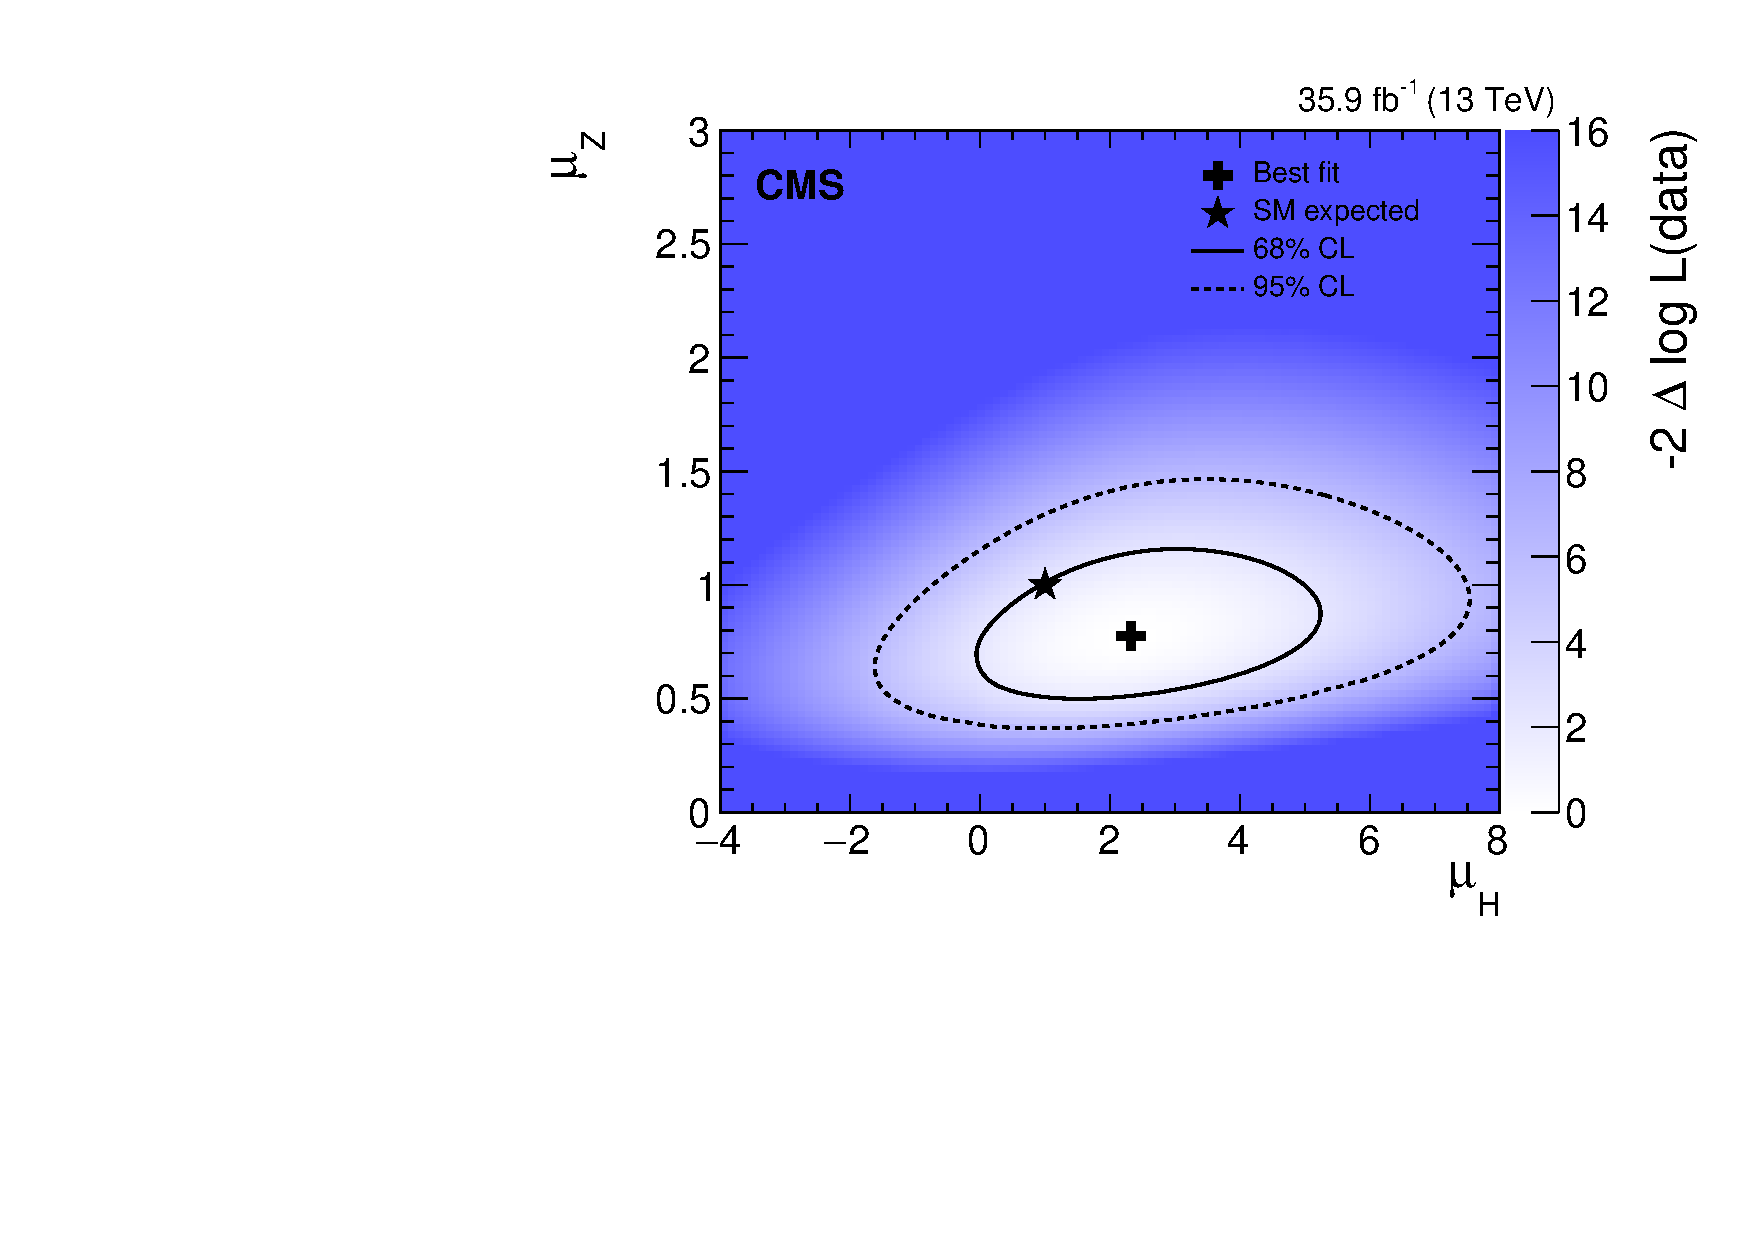
\includegraphics[width=0.55\textwidth]{figures/cms_SM_fittedH.pdf} \\
  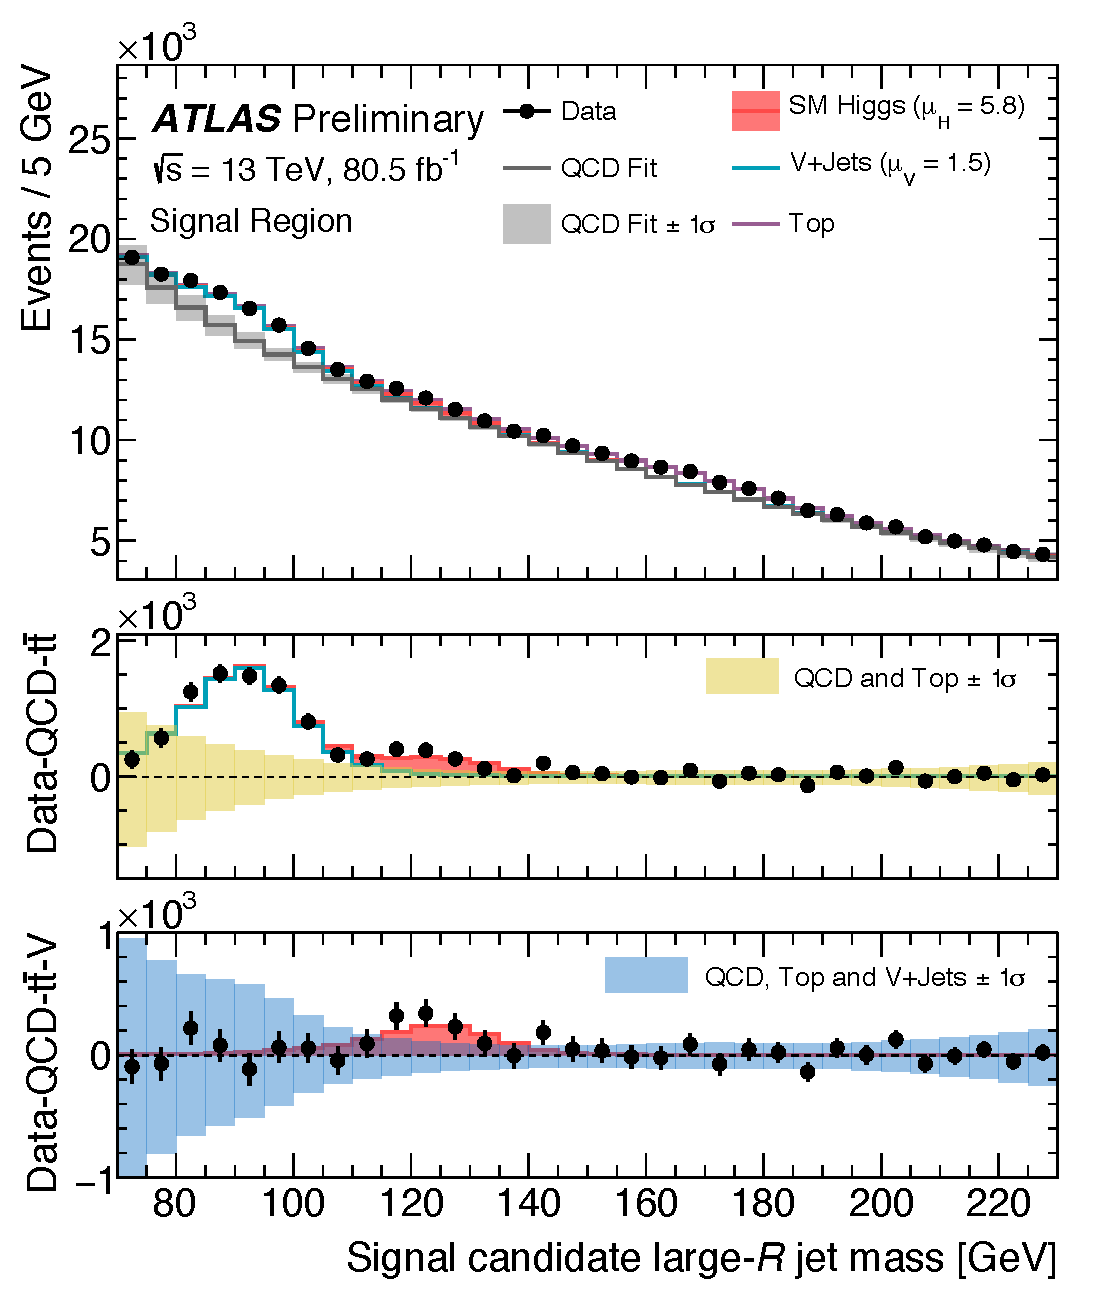
\includegraphics[width=0.45\textwidth]{figures/Hbb_ATLAS_dist.pdf}
    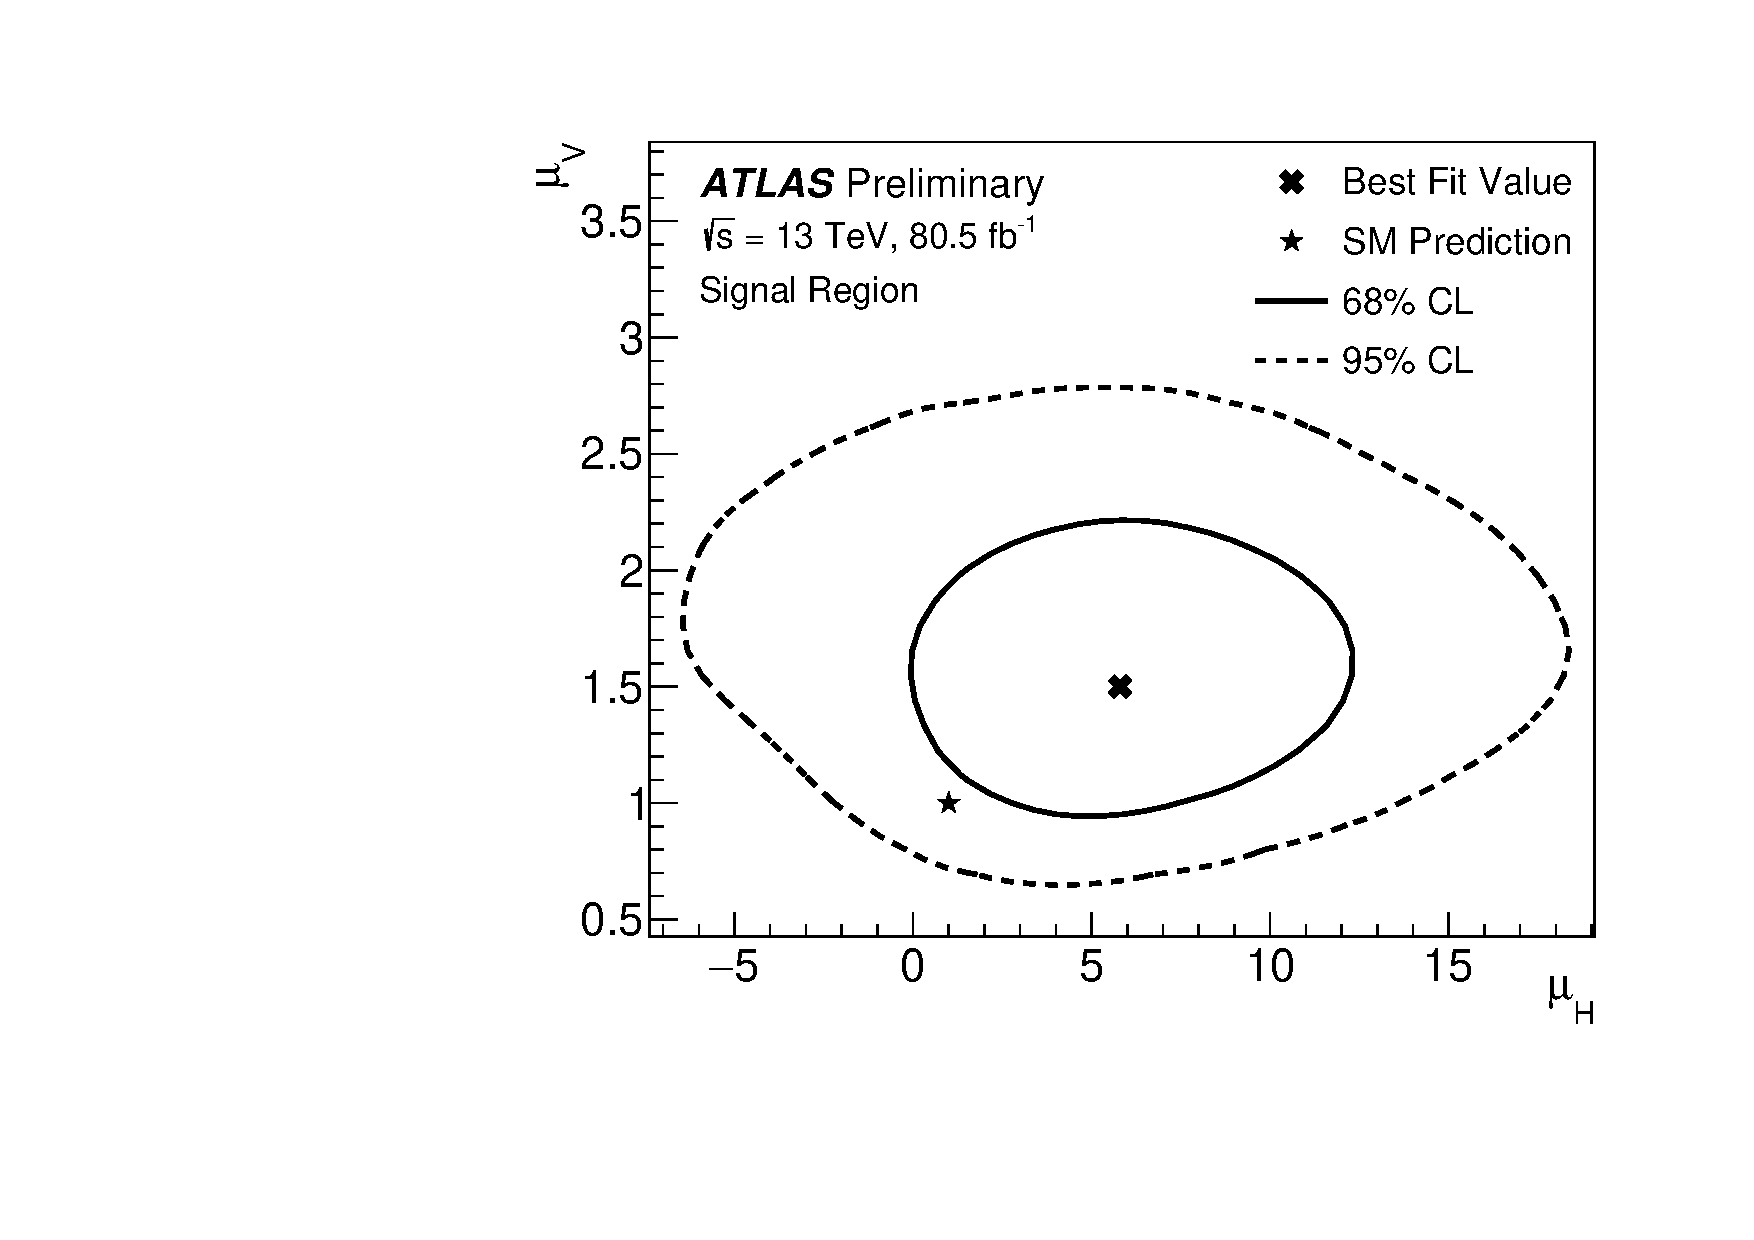
\includegraphics[width=0.55\textwidth]{figures/Hbb_ATLAS_fit.pdf}       
  \caption{Searches for boosted Higgs boson decaying into $b \bar b$. The plots show the invariant mass distribution and the signal-strength modification, top for CMS~\cite{Sirunyan:2017dgc}, bottom for ATLAS~\cite{ATLAS:2018hzj}.  }\label{fig:cms_boostedH}
\end{figure}

CMS performed an inclusive search for a Higgs boson decaying to $b\bar{b}$ pair, which is expected to result in an anti-$k_t$ $R=0.8$ jet, with $p_t \geq 450$ GeV \cite{Sirunyan:2017dgc}. The main experimental challenge originates in the large cross section for background multijet events at low jet mass. To increase the sensitivity for the reconstruction of the Z and Higgs boson \SD grooming is applied to the jet before two- and three-point generalised energy correlation functions are exploited to determine how consistent a jet is with having a two-prong structure. While a peak is clearly visible for the reconstruction of the Z boson, Fig.~\ref{fig:cms_boostedH} (top left) shows that the sensitivity to the Higgs boson still remains weak. However, it is already possible to set a limit on large signal-strength modifications to the production of either resonance, see Fig.~\ref{fig:cms_boostedH} (top right).

ATLAS has provided a similar measurement with an increased data set of $\mathcal{L} = 80.5~\mathrm{fb}^{-1}$ \cite{ATLAS:2018hzj}. To select the event, an anti-$k_t$ $R=1$ fat jet with $p_t \geq 480$ GeV is required. ATLAS is not showing the soft-drop groomed mass of the fat jet, but the invariant mass of trimmed jets. After subtracting the rather large QCD background a clear excess around the Higgs mass of $m_\text{H}=125$ GeV is observed, see Fig.~\ref{fig:cms_boostedH} (lower left panel). Small excesses around the Higgs and Z masses are indicative of an enhanced signal strength compared to the Standard Model predicted cross sections. Thus, ATLAS central value for the fit, allowing the signal strength for the V+jets and H+jets independently to float, is above the Standard Model value for either process, see Fig.~\ref{fig:cms_boostedH} (lower right panel). Yet, ATLAS and CMS 95\% exclusion contours both still contain the Standard Model value.

\section{Searches for new physics}

The kinematic situation outlined at the beginning of this book, cf Fig.~\ref{fig:resonance}, is common to many scenarios where the Standard Model is extended by heavy degrees of freedom. If such degrees of freedom descend from a model that addresses the hierarchy problem of the Higgs boson, they are likely to couple to the top quark and the bosons of the electroweak sector of the Standard Model, which in turn have a large branching ratio into jets. The conversion of energy from the heavy particle's rest mass into kinetic energy of the much lighter electroweak resonances causes them to be boosted in the lab frame. Thus, searches for new physics using jet substructure methods applied to fat jets can be amongst the most sensitive ways to probe new physics.

\subsection{Resonance decays into top quarks}
Top-tagging is the most active playground for the development of jet substructure classification techniques. A top jet has a rich substructure, providing several handles to discriminate it from the large QCD backgrounds, and due to the top quark's short lifetime its dynamics are to a large degree governed by perturbative physics. Thus, ATLAS and CMS have performed searches using a large variety of top-reconstruction techniques. 

New physics scenarios that are the focus of ATLAS and CMS searches contain models with extra dimensions or extended gauge groups, which give rise to heavy $\text{Z}'$ bosons, Kaluza-Klein gluons $g_{KK}$ and spin-2 Kaluza-Klein gravitons $G_{KK}$. The hadronic activity, and hence the tagging efficiency, depends on the quantum numbers of the heavy decaying resonance, in particular its colour charge~\cite{Joshi:2012pu}. These three resonances provide interesting benchmark points which can arise in many classes of new physics models. 

While ATLAS \cite{Aaboud:2018mjh} separates between a resolved and a boosted analysis in the semi-leptonic top-decay channel, i.e.\ with one top decaying leptonically ($t\to b \nu l^+$) and the other one hadronically ($t \to b j j$), CMS \cite{Sirunyan:2018ryr} focuses on the boosted regime but also considers the dileptonic and purely hadronic top decay modes. For the purpose of these notes, we are mostly interested in the boosted semi-leptonic top-decay mode, which suffers less from large dijet backgrounds, yet providing a larger signal cross section than the dileptonic channel.
ATLAS varies the resonance masses for the colour-singlet and colour-octet bosons with spin 1 or spin 2 between $0.4$ to 5 TeV and respectively their width between $1\%$ and $30\%$. To reconstruct the hadronic top, a large-$R$ jet is formed using the anti-$k_t$ algorithm with radius parameter $R=1.0$. This jet is trimmed to mitigate the effects of pileup and underlying event, using $R_\mathrm{sub} = 0.2$ and $f_\mathrm{cut}=0.05$. The resulting jets are required to have $p_t> 300$ GeV and $|\eta| < 2.0$. Such jets are then identified as top-tagged using the $N$-subjettiness ratio $\tau_{32}$ and an algorithm based on the invariant mass of the jet. The signal efficiency for this algorithm is found to be $80\%$. 

\begin{figure}[t]
  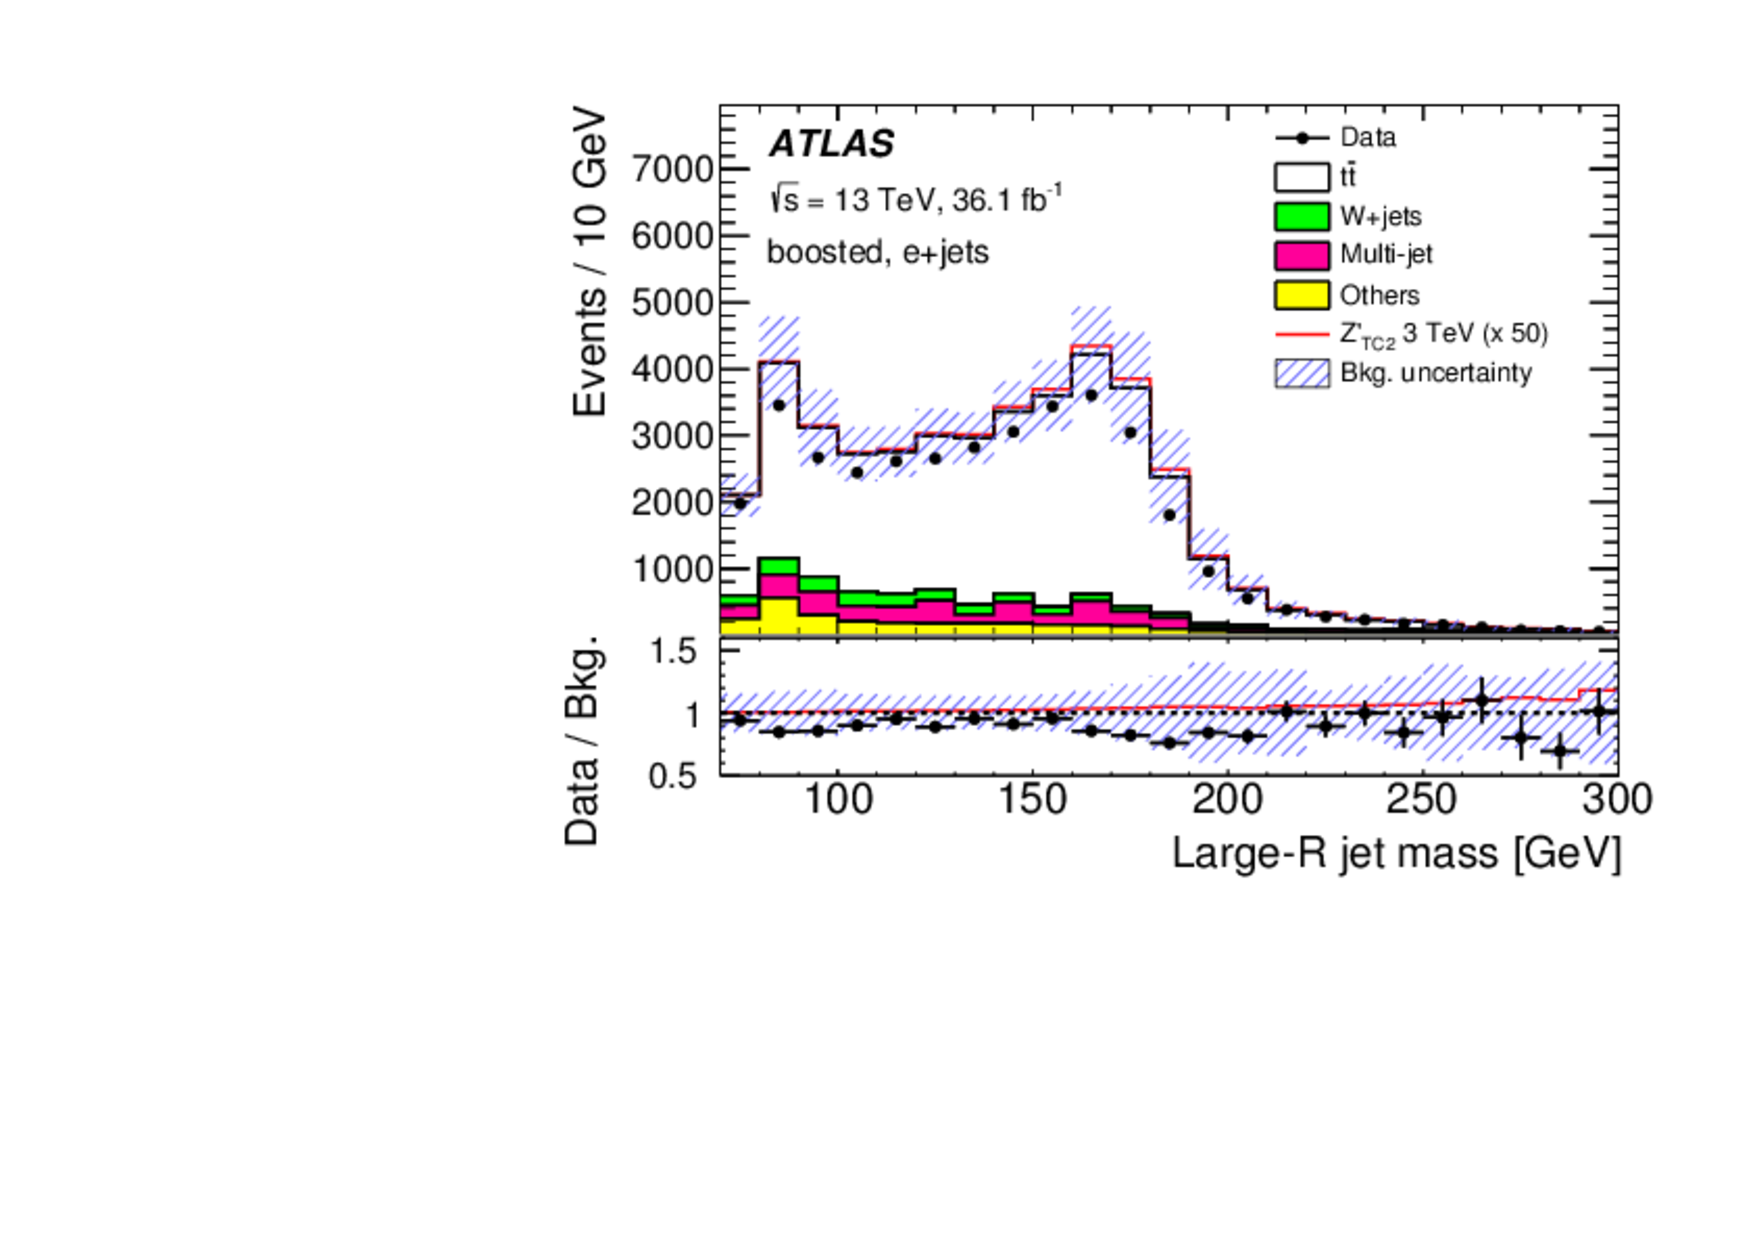
\includegraphics[width=0.45\textwidth]{figures/ATLAS_top_largeRjetmass.pdf}
  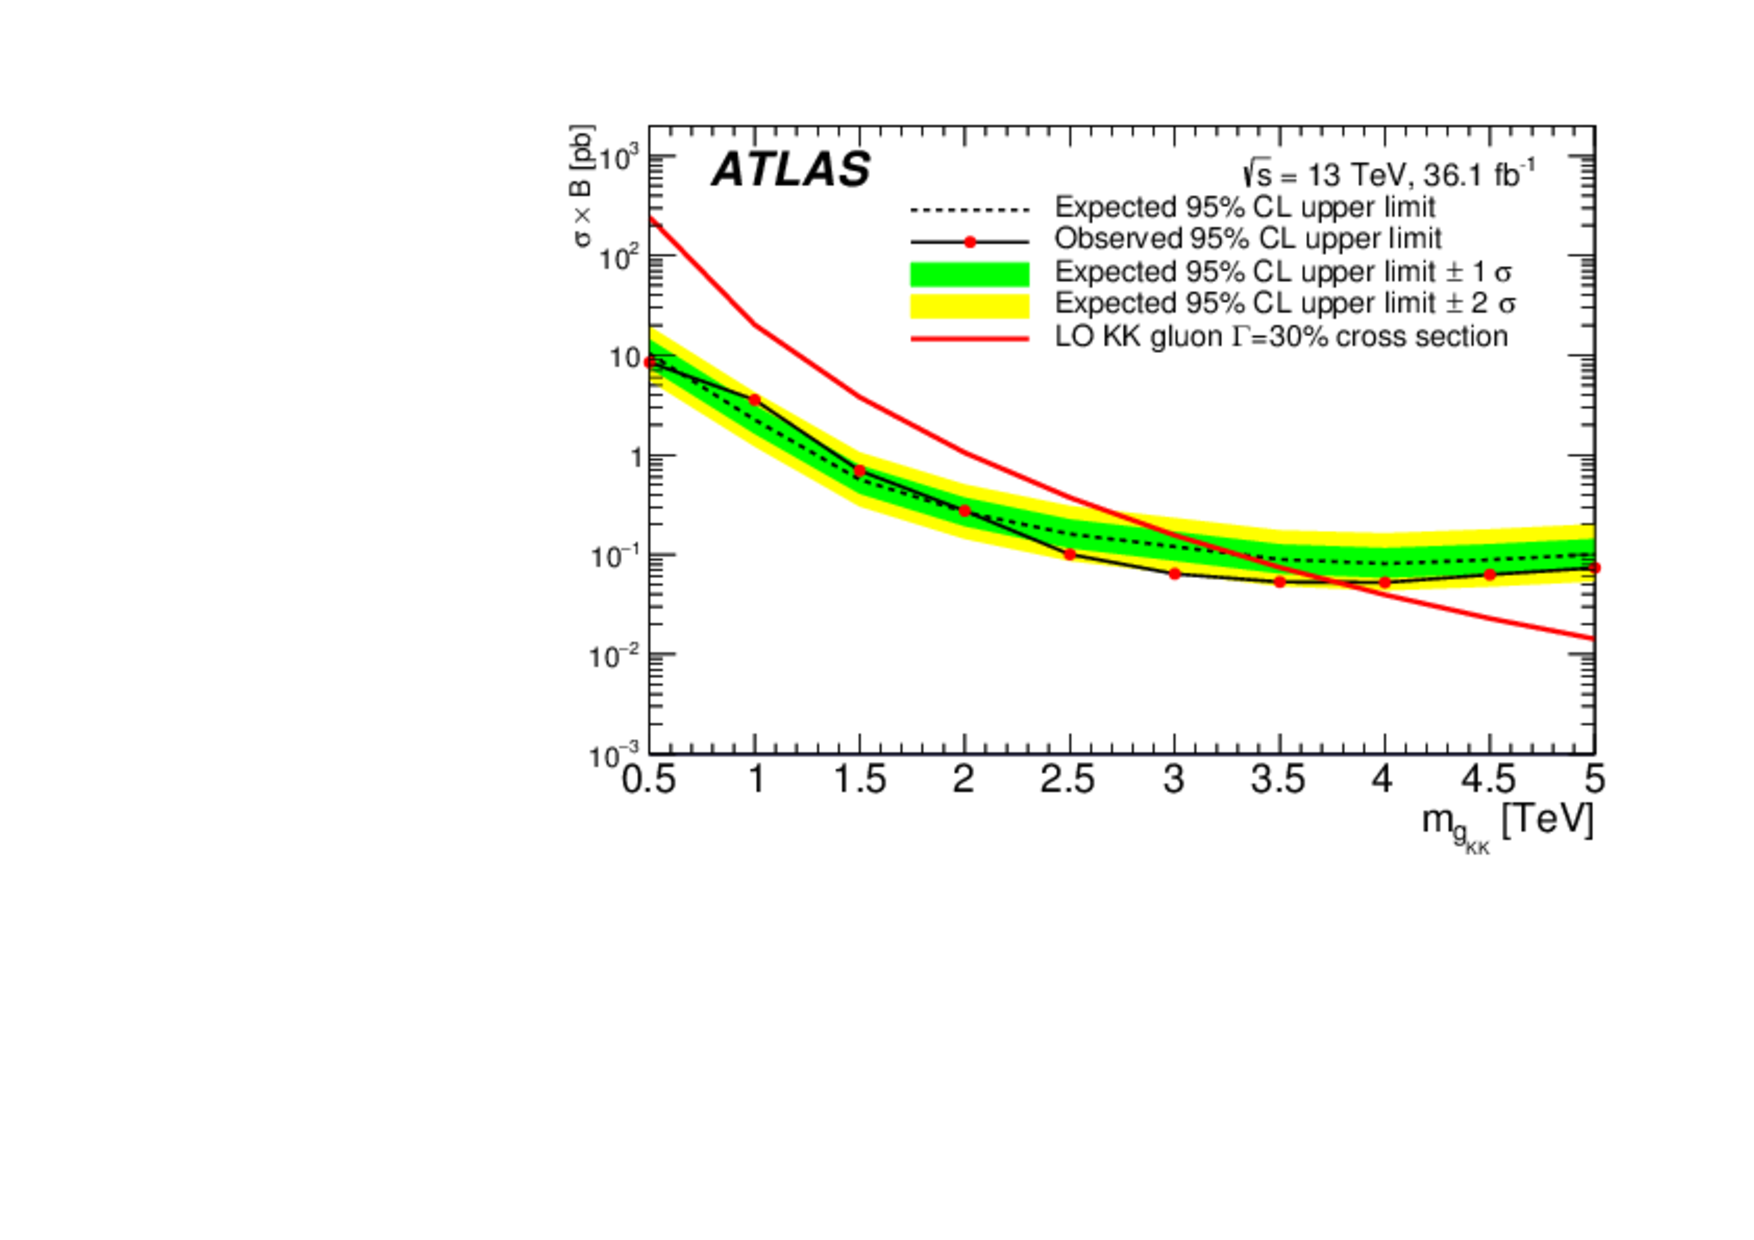
\includegraphics[width=0.5\textwidth]{figures/ATLAS_masslimit_tt_Gkk.pdf} \\
  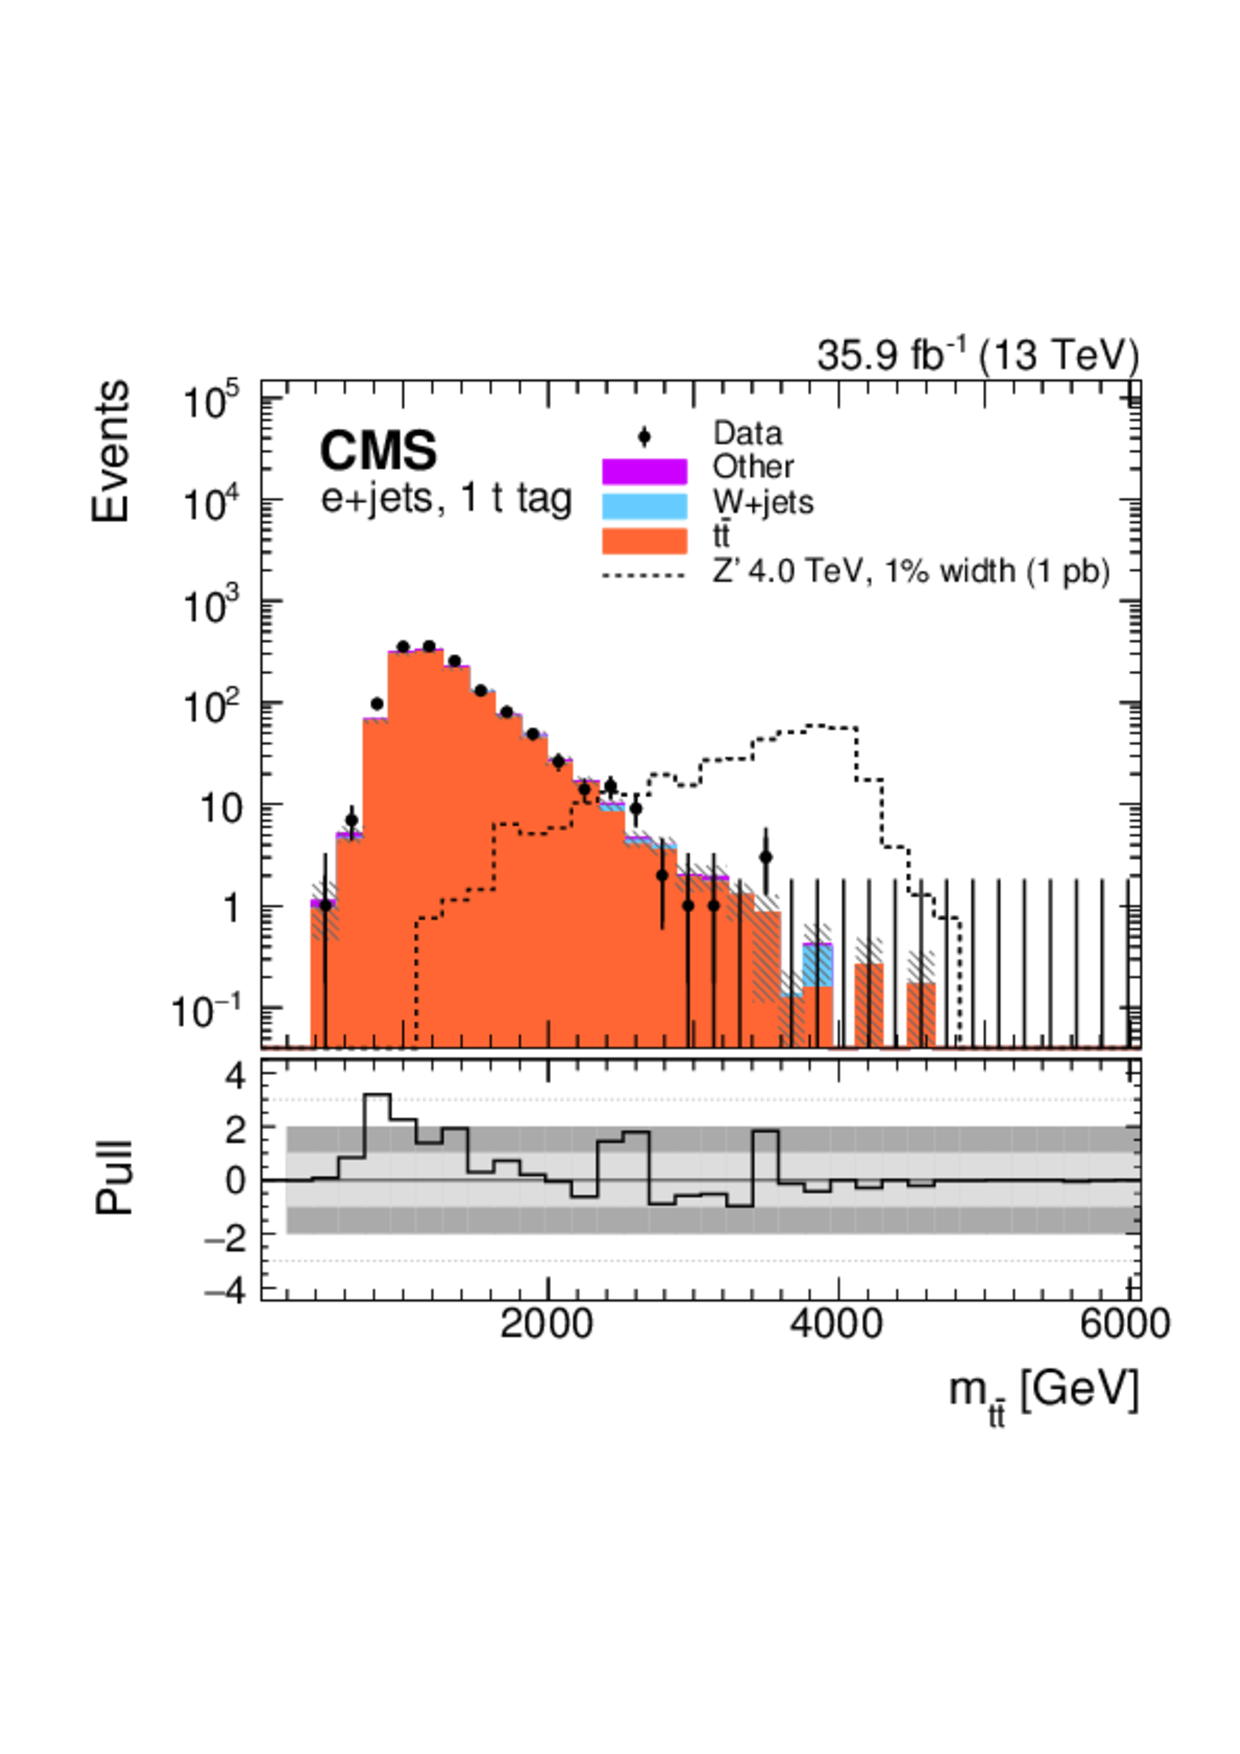
\includegraphics[width=0.45\textwidth]{figures/CMS_res_ttsemi.pdf}
  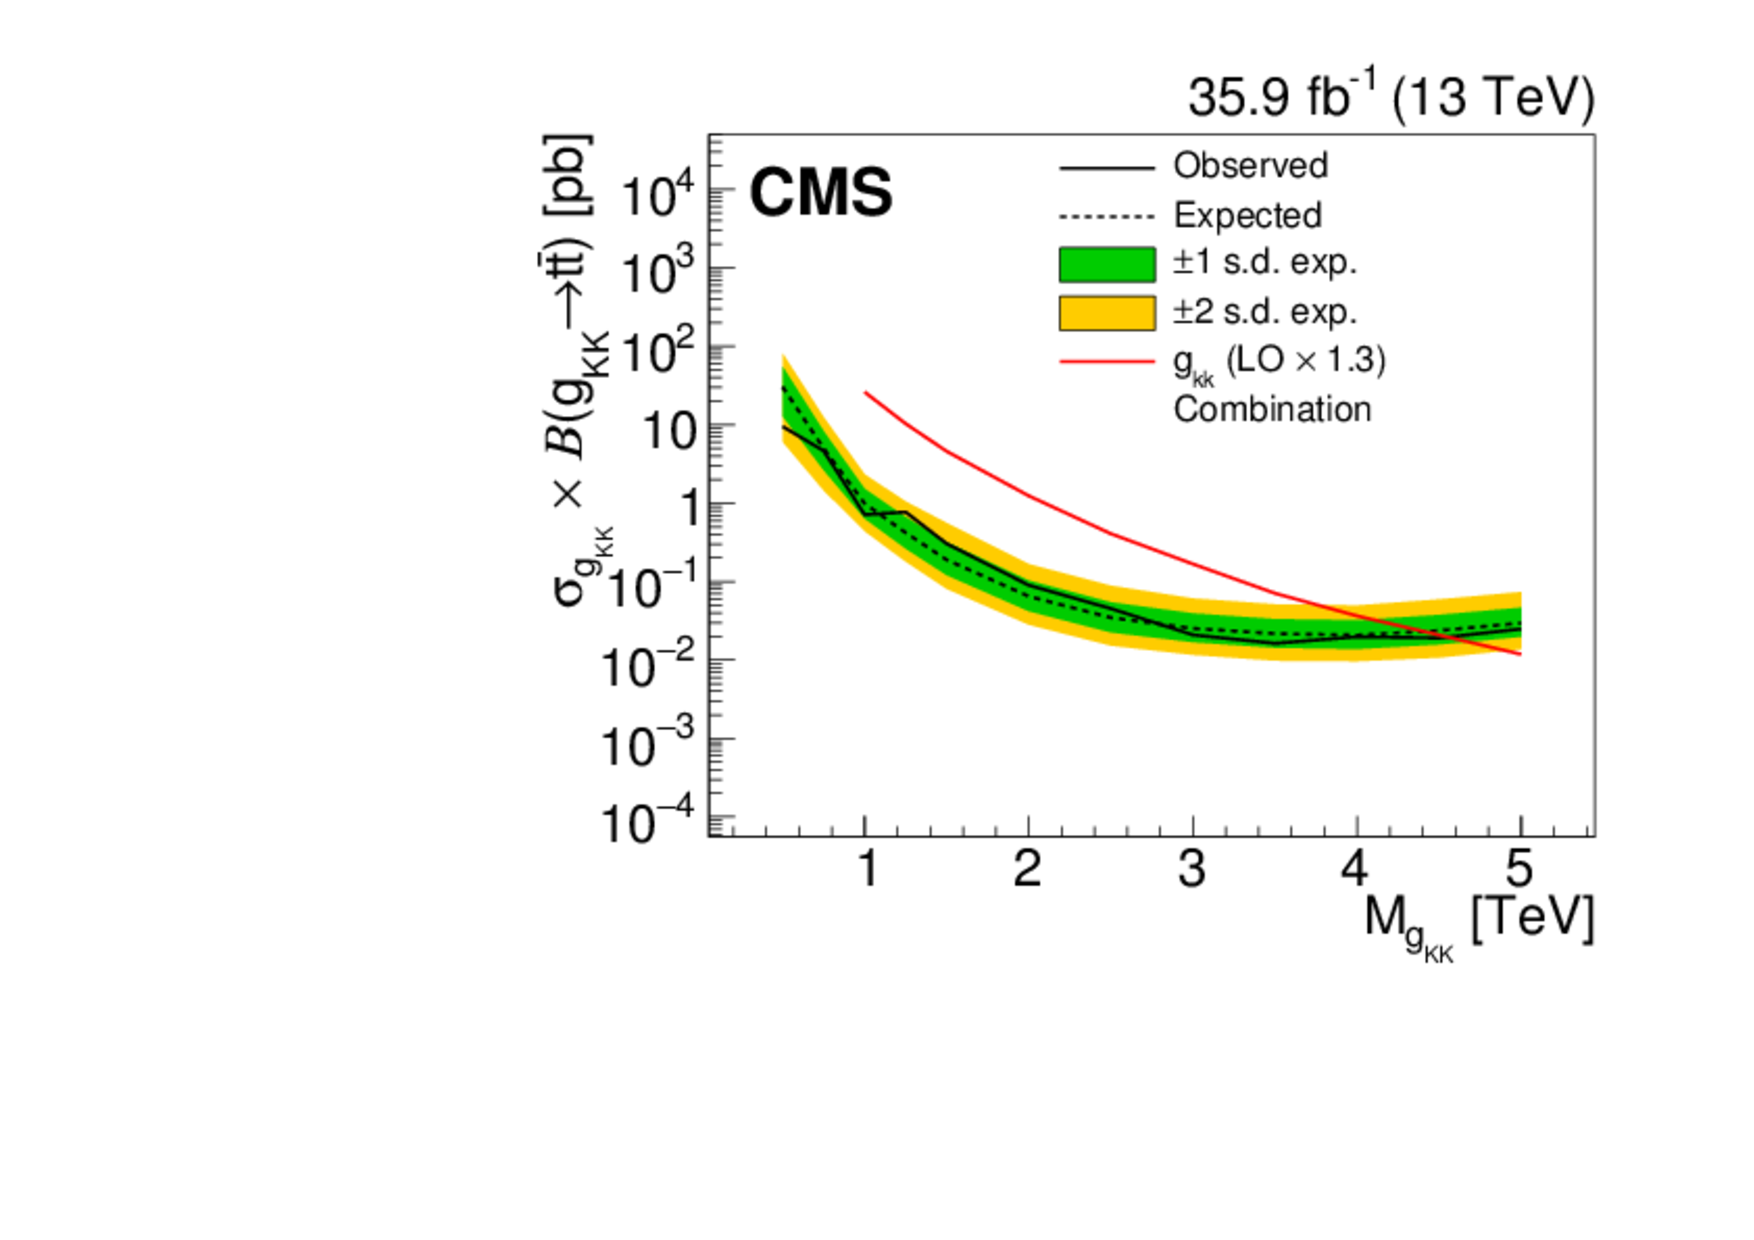
\includegraphics[width=0.5\textwidth]{figures/CMS_tt_gkk.pdf} 
  \caption{Searches for heavy resonances that involve top tagging from ATLAS~\cite{Aaboud:2018mjh}, on the top, and CMS~\cite{Sirunyan:2018ryr} on the bottom. }\label{fig:res_ttdecays}
\end{figure}

For the same task CMS uses somewhat smaller anti-$k_t$ $R=0.8$ jets. These jets receive pileup per particle identification (PUPPI) \cite{Bertolini:2014bba} corrections. The top tagging algorithm then only considers jets with $p_t > 400$ GeV to ensure a collimated decay of the top quark. 
The top tagging algorithm then includes a grooming step, performed with \SD $\beta=0$, i.e.\ mMDT, algorithm, with $z_\mathrm{cut} = 0.1$ and $R_0 = 0.8$ and a cut on the $N$-subjettiness ratio $\tau_{32}$. The \SD mass is then required to be close enough to the true top mass, i.e. $105 < m_{\mathrm{SD}} < 210$ GeV and $\tau_{32}$ must be less than 0.65. 

The reconstruction techniques applied show a very good agreement between the measured data and the Monte-Carlo predicted pseudo-data, Fig.~\ref{fig:res_ttdecays} (left panels). With only $36~\mathrm{fb}^{-1}$, depending on the resonance's couplings and width, heavy resonances decaying into top quarks can be excluded up to mass of 3.5 TeV, Fig.~\ref{fig:res_ttdecays} (right panels). For such large masses jet-substructure methods are not optional. Without using the internal structure of jets the QCD-induced dijet backgrounds would overwhelm the signal.

In models where the $\text{Z}'$ arises from to a SU(N) gauge group, it will be accompanied by a $\text{W}'$. ATLAS \cite{Aaboud:2018juj} has performed searches for heavy $\text{W}'$ decaying into a hadronic top and a bottom quark, i.e. $\text{W}' \to t  \bar{b} \to q \bar{q} b \bar{b}$. This search is somewhat more intricate than the searches for decays into two top quarks as there are fewer handles to suppress the backgrounds. Thus, ATLAS uses the shower deconstruction top tagging algorithm, discussed in Sec.~\ref{shower_dec}, which has a strong rejection power of QCD jets while maintaining a large signal efficiency. ATLAS finds a working point of the tagger with $50\%$ signal efficiency and a background rejection factor of 80, thus improving the signal-to-background ratio by a factor 40, for anti-$k_t$ $R=1.0$ jets with $p_t>450$ GeV. 
%
\begin{figure}
  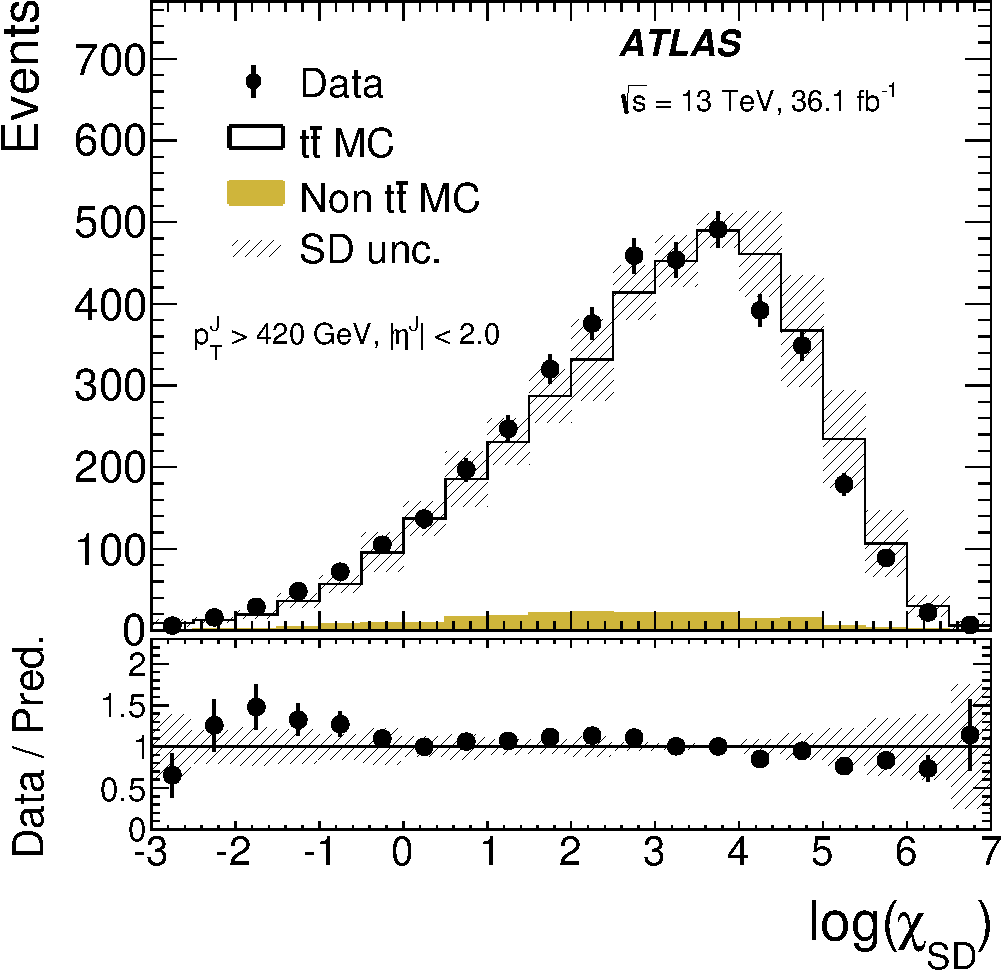
\includegraphics[width=0.4\textwidth]{figures/ATLAS_Wprime_data.pdf} 
  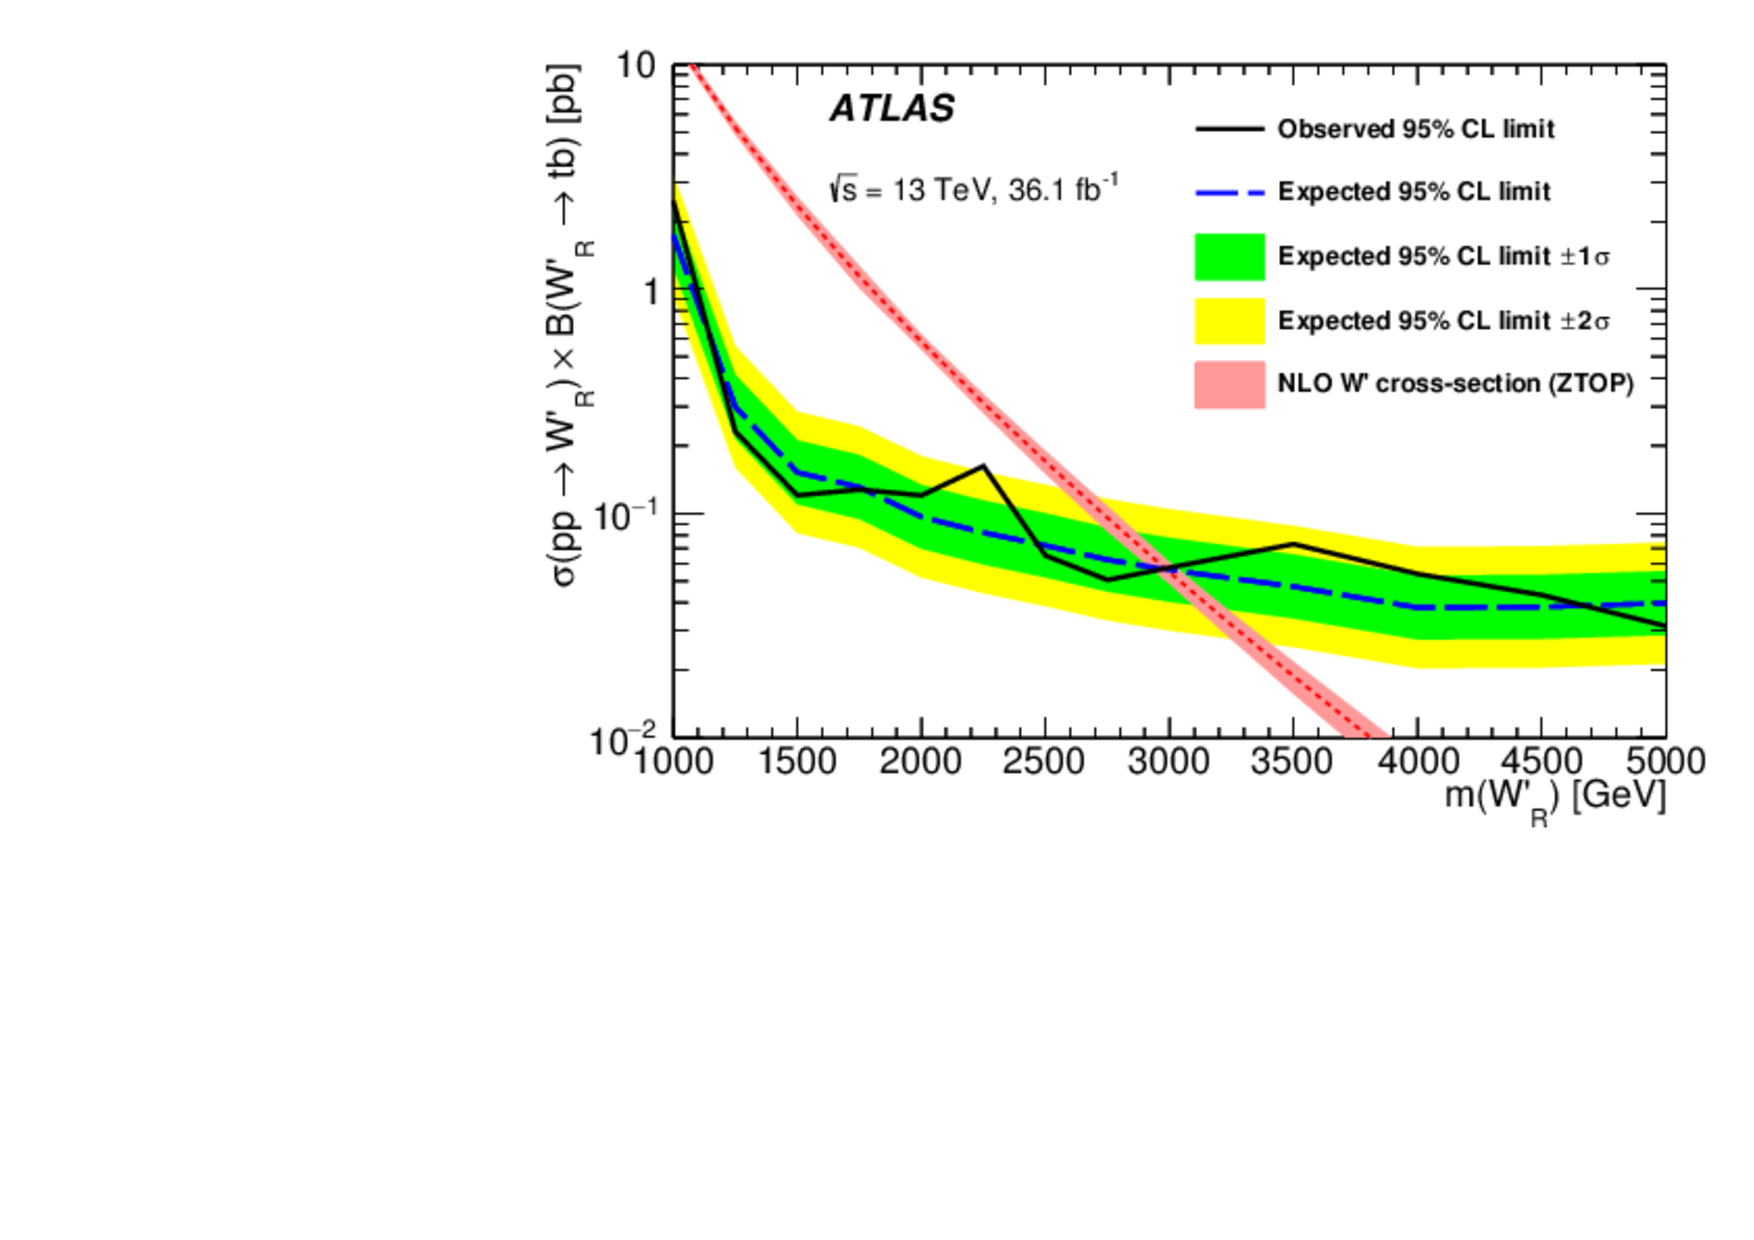
\includegraphics[width=0.6\textwidth]{figures/ATLAS_WR_exclusion.pdf}
  \caption{Search for a $\text{W}'$ performed by ATLAS~\cite{Aaboud:2018juj} using shower deconstruction.}\label{fig:Wprime_excl}
\end{figure}
%
Applied to $t\bar{t}$ events the shower deconstruction algorithm shows very good agreement between data and Monte-Carlo simulated pseudo-data, Fig.~\ref{fig:Wprime_excl} (left). After applying the top tagger and reconstructing the final state in the search for a $\text{W}'$, ATLAS can exclude masses up to 3 TeV, Fig.~\ref{fig:Wprime_excl} (right). The sensitivity does not depend on whether the $\text{W}'$ couples to left or right-handed quarks.



\subsection{Resonance decays into Higgs and gauge bosons}
Currently, most of the resonance searches into electroweak bosons that are using jet substructure techniques are focusing either on heavy resonances decaying into Higgs bosons, with subsequent decay into bottom quarks \cite{Aad:2015uka, Sirunyan:2017isc, Sirunyan:2018qca}, or decays into W and Z bosons, with subsequent decay into quarks \cite{Aad:2015owa, Khachatryan:2014hpa}.
The new physics scenarios studied range from the decay of a Kaluza-Klein excitation of the graviton in the bulk Randall-Sundrum model with a warped extra dimension \cite{Agashe:2007zd}, over the decay of a $CP$-even heavy Higgs boson, as present in two-Higgs double models (2HDM) \cite{Branco:2011iw}, to a heavy scalar from a triplet-Higgs model, e.g.\ the so-called Georgi-Machacek model \cite{Georgi:1985nv}. In general one assumes a heavy resonance in the range $m_X \gtrsim 500$ GeV is produced, with a short lifetime. While the spin of the resonance could be in principle studied by reconstructing and analysing the decay planes of the quark pairs \cite{Hackstein:2010wk, Englert:2010ud}, at this point such attempts are not being made and the separation between signal and background, after reconstructing the electroweak bosons, relies entirely on the presence of a bump in their invariant mass distribution. Thus, the width in combination with the mass of the decaying resonance is of great importance for its discovery or exclusion.


To reconstruct the Higgs boson pairs from a heavy resonance decay ATLAS \cite{Aad:2015uka, ATLAS:2016ixk} considers a resolved and a boosted analysis. In the boosted case, Higgs bosons are selected by requiring that two large-$R$, i.e. anti-$k_t$ $R=1.0$ with $p_t \geq 250$ GeV, have each two $b$-tags, and that the leading fat jet has in addition $p_t \geq 350$ GeV. The backgrounds are derived from Monte-Carlo simulations. For a resonance width of $\Gamma = 1$ GeV, in combination with the resolved analysis, this results in an 95\% C.L. exclusion for a bulk Randall-Sundrum graviton with coupling value $k/\tilde{M}_{PL}=2$, where $\tilde{M}_{\mathrm{PL}}$ is the reduced Planck mass, of $500 \leq m_{G^*_{KK}} \leq 990$ GeV, see Fig.~\ref{fig:X_HH} (left). With the integrated luminosity used in this analysis, the resolved analysis is more sensitive than the boosted analysis up to $m_{G^*_{KK}} \leq 1100$ GeV.

CMS \cite{Sirunyan:2018qca} in a search at $\sqrt{s} = 13~\mathrm{TeV}$ with 35.9 $\mathrm{fb}^{-1}$ aims for the exclusion of heavier masses and instead uses anti-$k_t$ $R=0.8$ jets with $p_t \geq 350$ GeV. The resulting fat jet is groomed using the \SD algorithm with $z=0.1$ and $\beta=0$ (mMDT). The groomed jet mass is required to have $105 \leq m_{\mathrm{sd}} \leq 135$ GeV. To suppress QCD backgrounds further, the N-subjettiness algorithm is used, requiring $\tau_{21} < 0.55$. Eventually, each of the jets is double-$b$ tagged, which has the largest impact on the backgrounds. After searching for a bump in the invariant mass spectrum of the two fat jets, CMS obtains a 95\% C.L. exclusion for a bulk radion with mass $970 < m_R < 1400$ GeV, see Fig.~\ref{fig:X_HH} (right).

\begin{figure}
  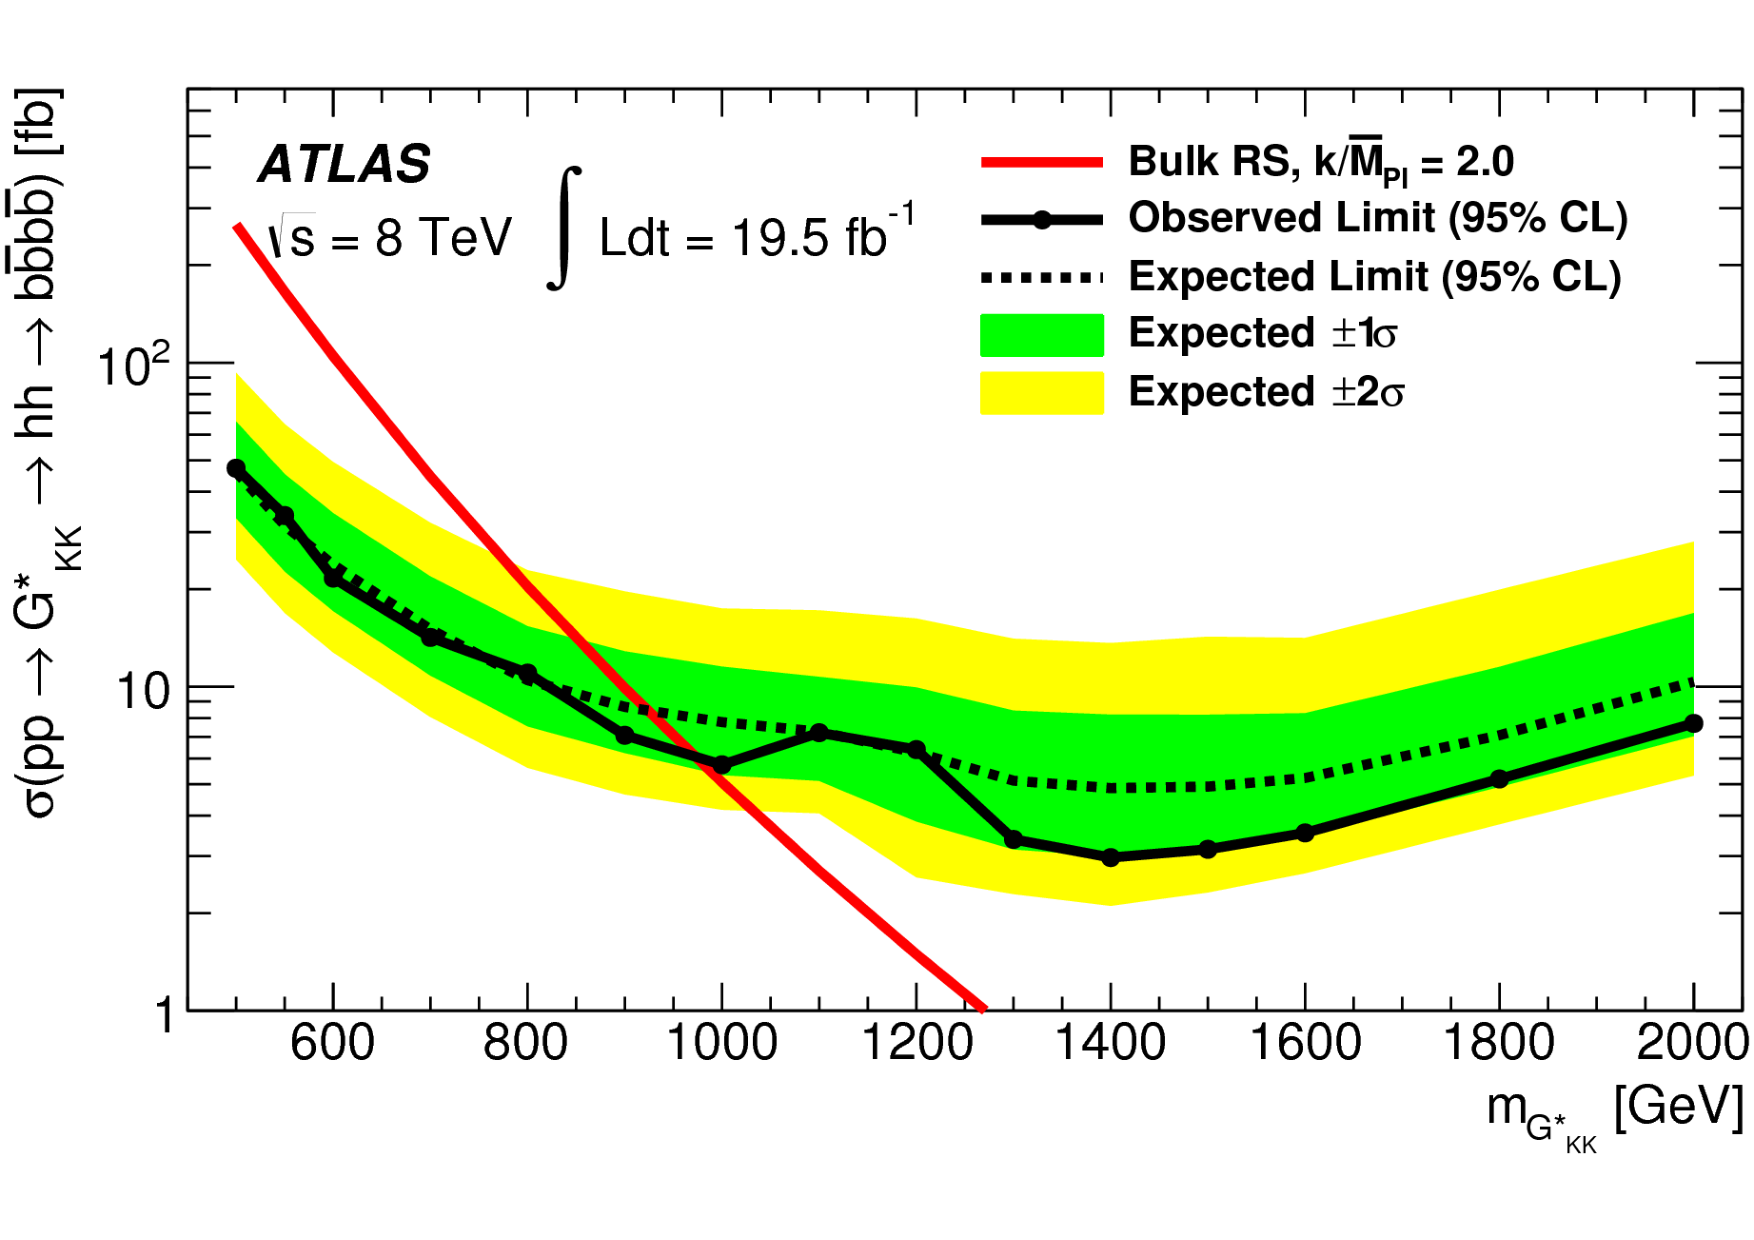
\includegraphics[width=0.48\textwidth,trim=0 20 0 40]{figures/ATLAS_X_HH.pdf}\hfill
  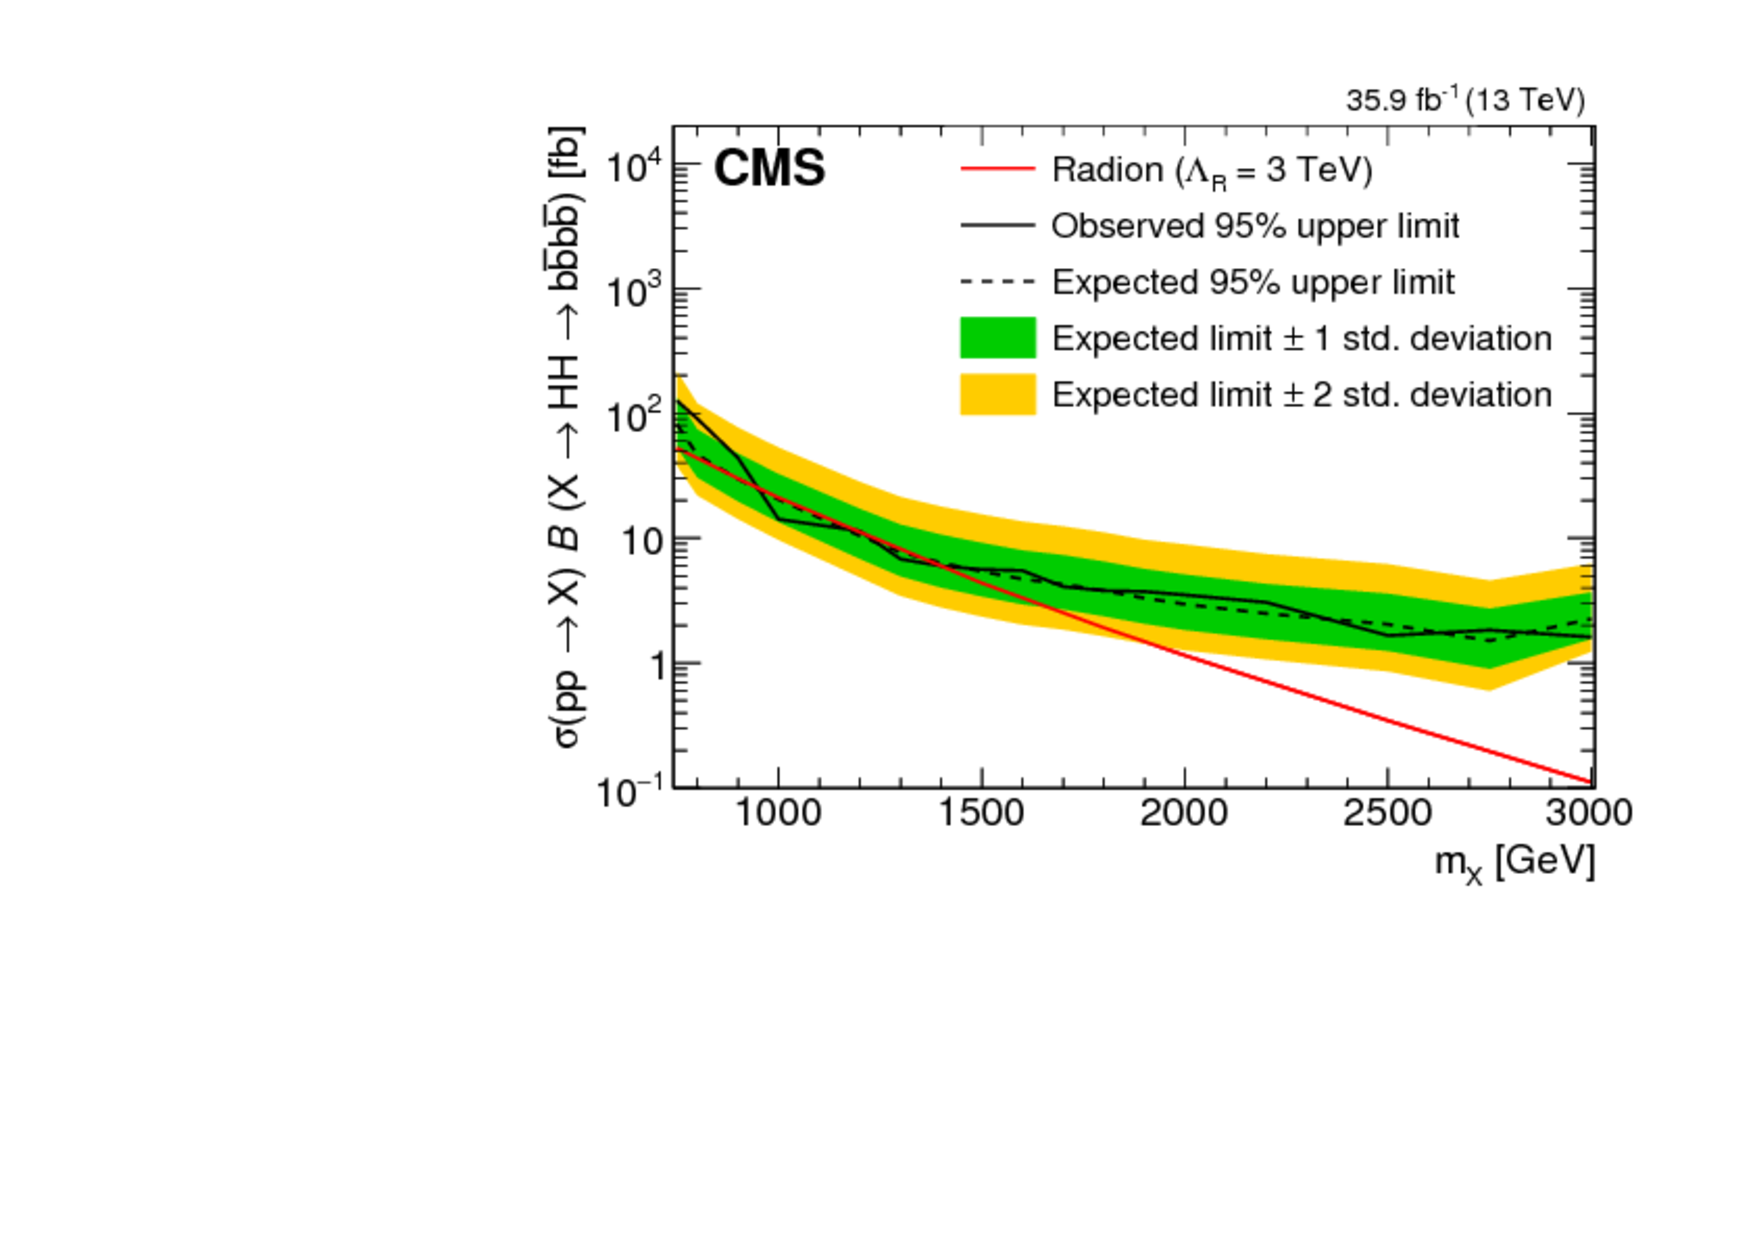
\includegraphics[width=0.45\textwidth,trim=0 37 0 20]{figures/CMS_X_HH.pdf} 
  \caption{Example of exclusions limits from searches of resonances decaying into two Higgs bosons, the ATLAS search of Ref.~\cite{Aad:2015uka} is shown on the left, while the CMS search of Ref.~\cite{Sirunyan:2018qca} on the right. }\label{fig:X_HH}
\end{figure}

The decay of a heavy resonance into gauge bosons is a frequent feature of many extensions of the Standard Model. For example, the aforementioned bulk graviton could decay into a pair of W or Z bosons, or a heavy gauge boson of an additional or extended gauge group, a so-called W$'$ or Z$'$, can decay into the pairs of Standard Model gauge bosons. In \cite{Aad:2015owa, Khachatryan:2014hpa} ATLAS and CMS have both observed a small excess in dijet final states, where each jet was W/Z tagged. The excess resided at a similar invariant mass range of $m_{jj} \sim 2$ TeV, but was slightly more significant in the ATLAS analysis.
In this search, at $\sqrt{s}=8$ TeV, ATLAS selected two fat jets with Cambridge/Aachen algorithm $R = 1.2$, with a minimal transverse momentum of $p_t  \geq 540$ GeV. The reconstruction of the gauge bosons relied on a combination of a jet-mass cut around the masses of the weak gauge bosons and grooming techniques, where a modified version of the BDRS reconstruction technique \cite{Butterworth:2008iy} was employed\footnote{As discussed in \cite{Krauss:2014yaa}, the way the BDRS approach was modified in the search by ATLAS could result in shaping the $m_{VV}$ distribution in the region of 2 TeV, where the excess was observed.}, a method initially designed for the reconstruction of a Higgs boson with $p_{t,\text{H}} \geq 200$ GeV. Using this approach, the mass resolution of the reconstructed gauge boson is not good enough to discriminate between W and Z bosons. Eventually, to improve on the separation of signal and background, cuts were applied on the momentum ratios of subjets, the number of charged particles within a subjet and the mass of the reconstructed gauge bosons. After recombining the four-momenta of the two reconstructed gauge bosons an excess was observed in the mass range $1.9 \leq m_\text{VV} \leq 2.1$ TeV over the data-driven (fitted) background estimate, mainly driven by the QCD background, see Fig.~\ref{fig:X_VV}.

CMS reconstructed the W and Z bosons by applying the pruning algorithm as a groomer and tagger for the fat jet. To further improve the separation between $W/Z$ bosons and QCD jets $\tau_{21}$ was used. Both experiments find an excess at $\sim 1.9$ TeV, whereas the excess in ATLAS with $2.8 \sigma$ is more pronounced than in CMS with $1.8 \sigma$. Both experiments have updated this search using different reconstruction strategies and with more statistics, which eventually dampened the excess strongly \cite{Aaboud:2017eta, Sirunyan:2017acf}.


\begin{figure}
  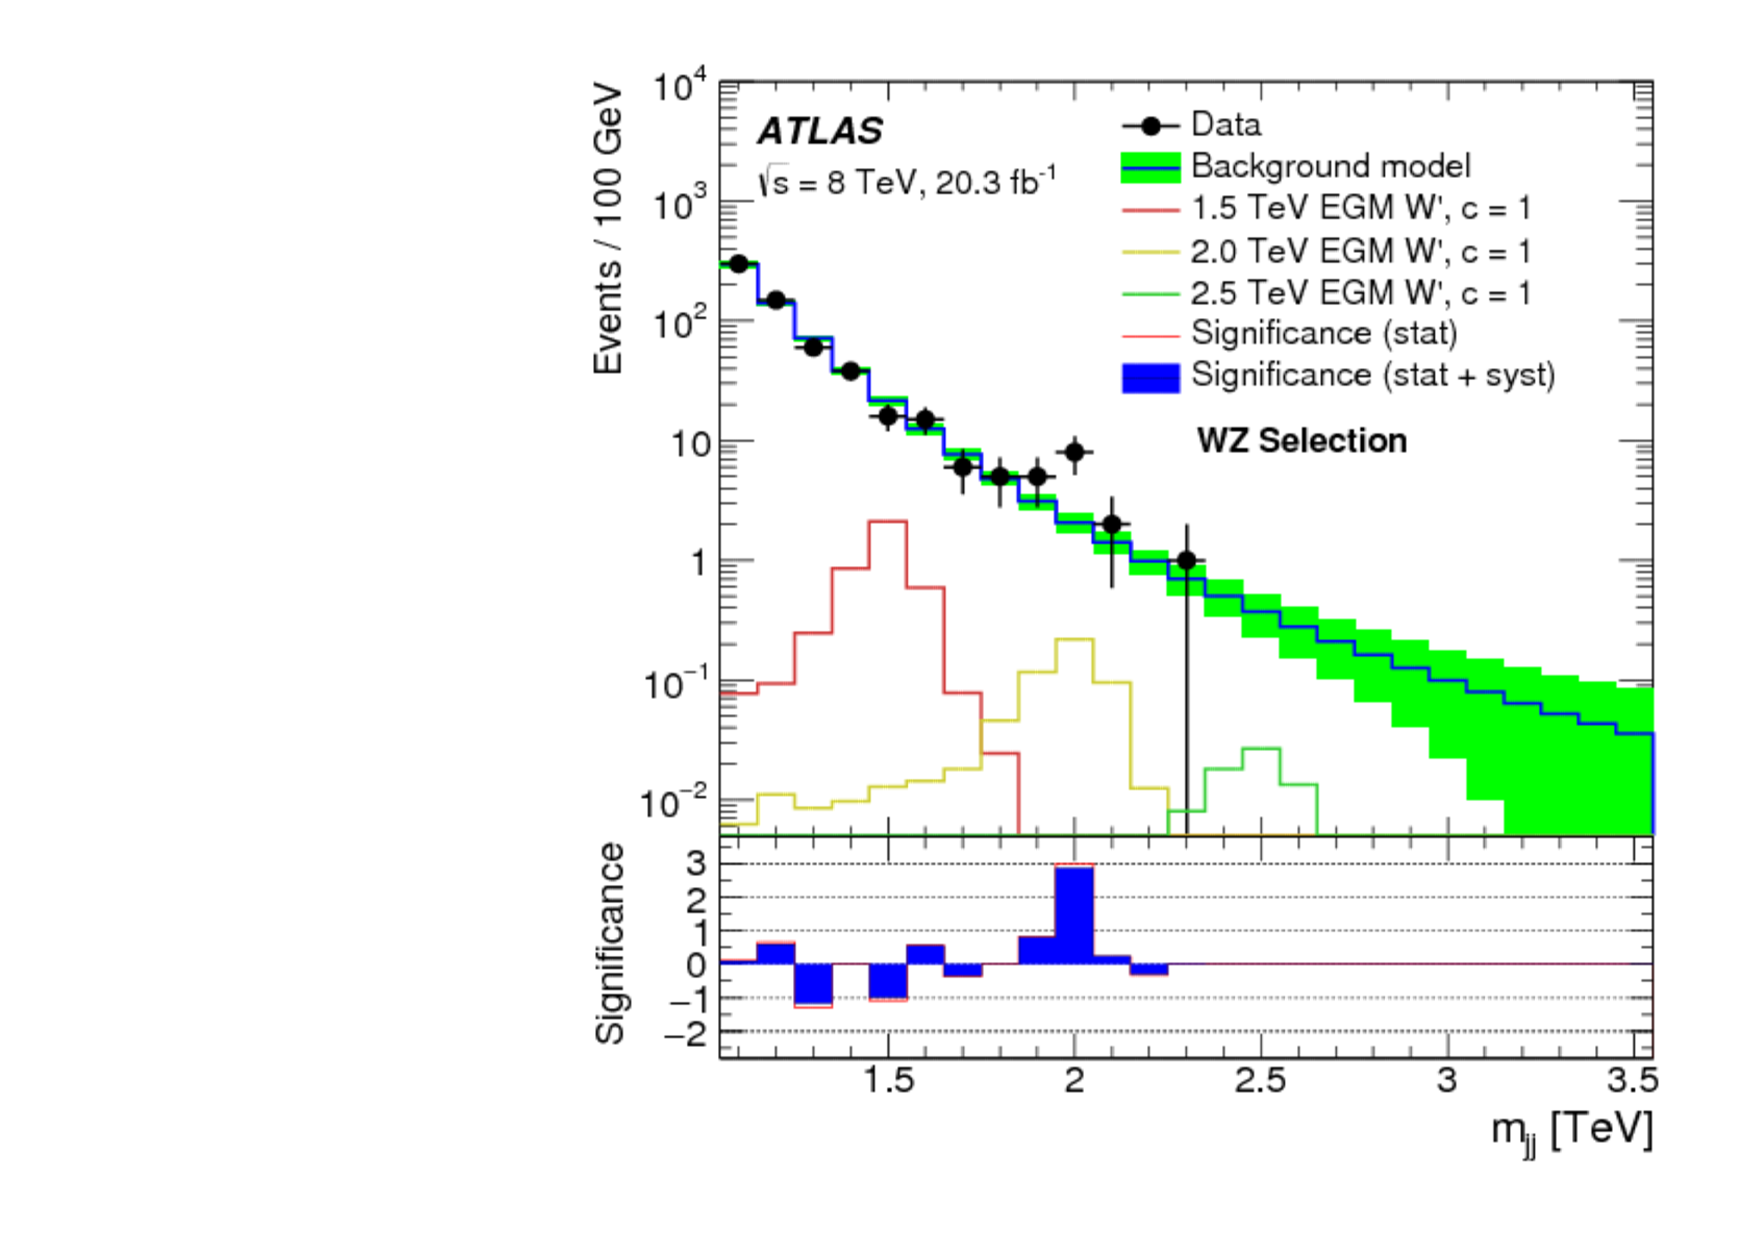
\includegraphics[width=0.45\textwidth]{figures/ATLAS_Wp_WZ.pdf} 
  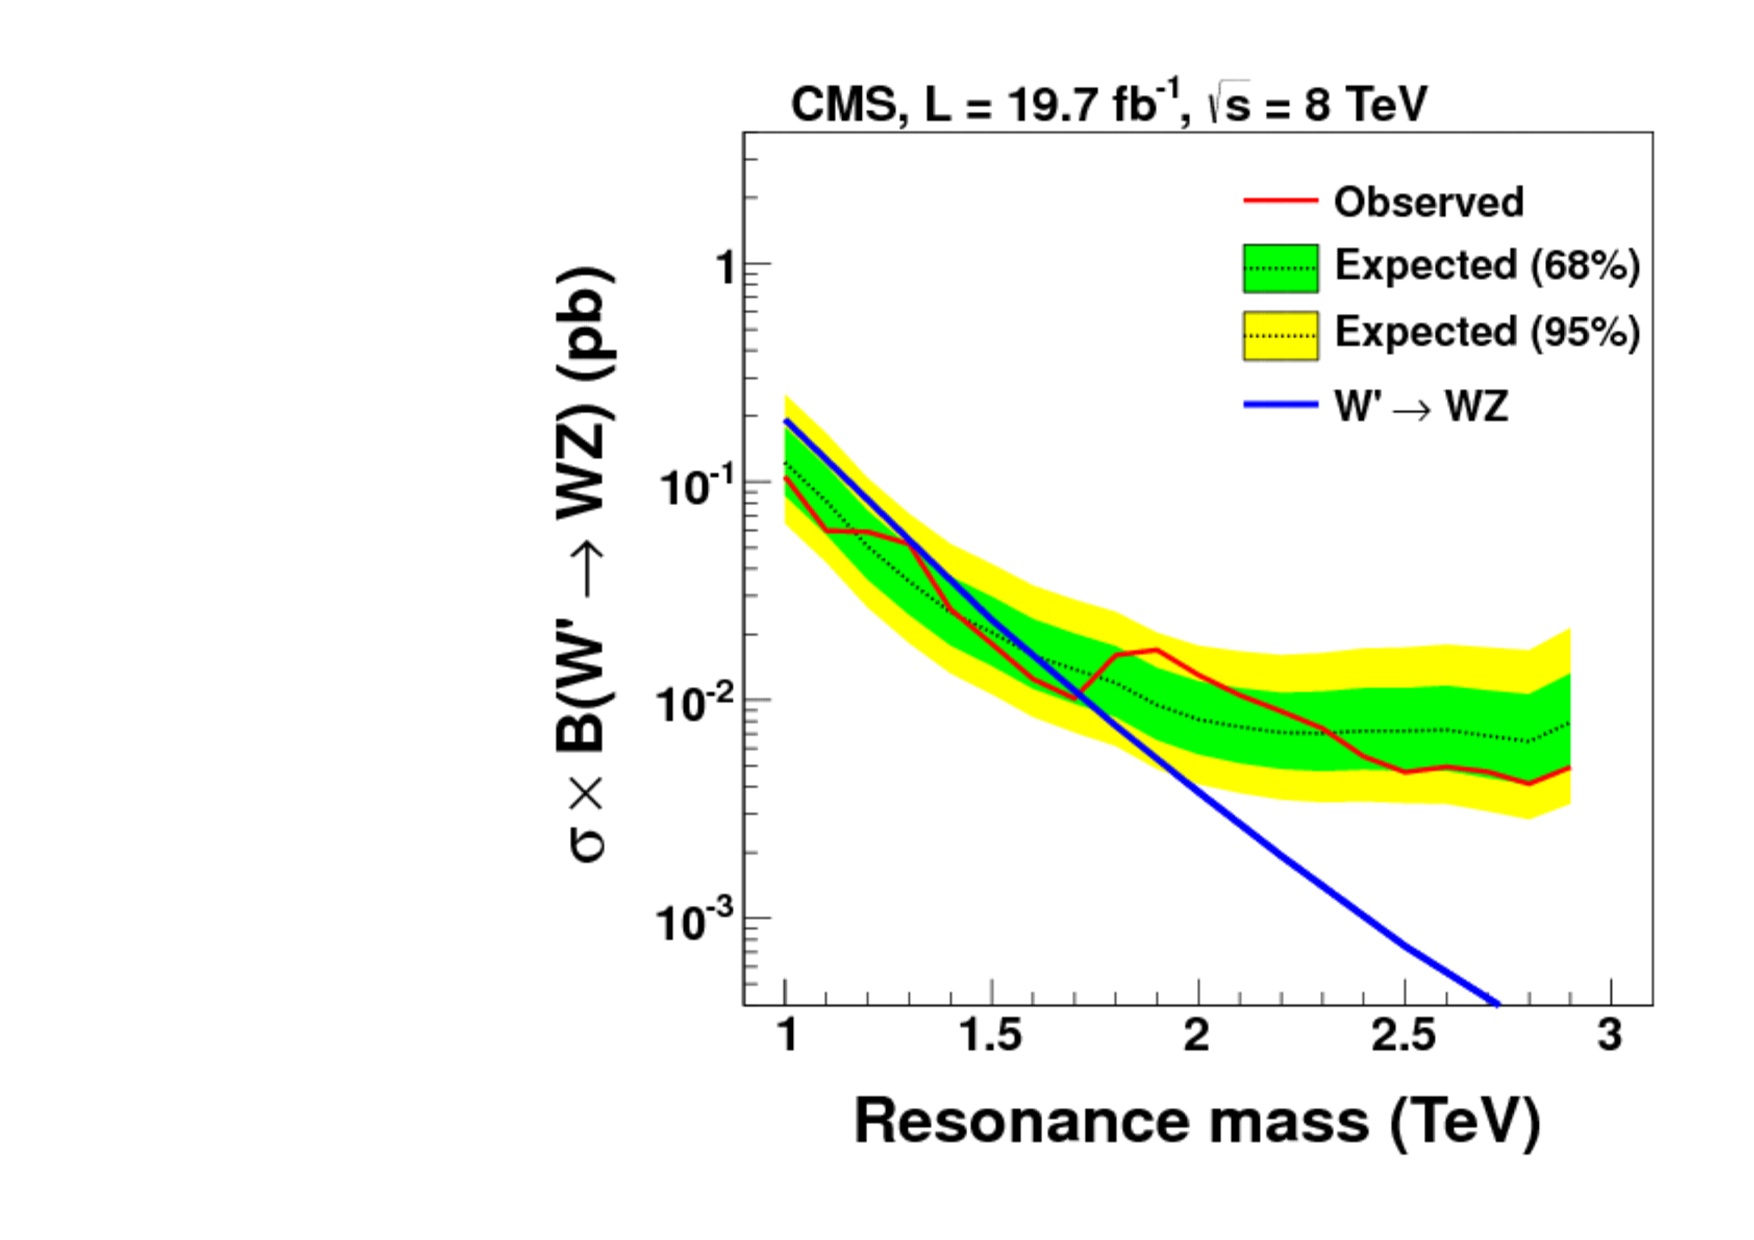
\includegraphics[width=0.45\textwidth]{figures/CMS_W_WZ.pdf} 
  \caption{Invariant mass distribution of the reconstructed gauge bosons as measured by ATLAS \cite{Aad:2015owa}, on the left, and the exclusion limit for a $\text{W}'$ decaying into WZ set by CMS \cite{Khachatryan:2014hpa} on the right.}\label{fig:X_VV}
\end{figure}



\subsection{Resonance decays into new particles}

If a heavy resonance decays via electroweak resonances of the Standard Model into quarks or gluons the masses of the Standard Model particles themselves provide an important handle to separate signal from background. This task is however complicated if the intermediate resonances are not known, e.g.\ when a squark decays into four quarks through an intermediate Higgsino with a hadronic R-parity-violating coupling \cite{Butterworth:2009qa}. CMS has performed searches for squarks via such a decay mode \cite{CMS:2018sek} and ATLAS a similar study in \cite{Aad:2016kww}. 

Without knowing the mass of the Higgsino, CMS in \cite{CMS:2018sek} uses the fact that a squark decays into a four-pronged object to discriminate signal from background. In order to capture as many of the final-state constituents of the squark decay products as possible, large Cambridge/Aachen ($R=1.2$) jets are formed. These jets are analysed using the $N$-subjettiness ratios, requiring $\tau_{43}<0.8$ and $\tau_{42}<0.5$ for each jet. As pair production of the squarks is assumed, the masses of the reconstructed fat jets should not be too asymmetric, i.e. $|m_1 - m_2| / (m_1+m_2) < 0.1$. After defining the average jet mass as $\bar{m} = (m_1+m_2)/2$ CMS finds very good agreement between the theoretically predicted background cross sections and the measured data, see Fig.~\ref{fig:X_search} (left). This allows to set an exclusion limit in this channel requiring squark masses to be $m_{\tilde{q}}  > 720$ GeV, when assuming that the Higgsino mass is $m_{\tilde{H}} = 0.75 m_{\tilde{q}}$, Fig.~\ref{fig:X_search} (right).


\begin{figure}
  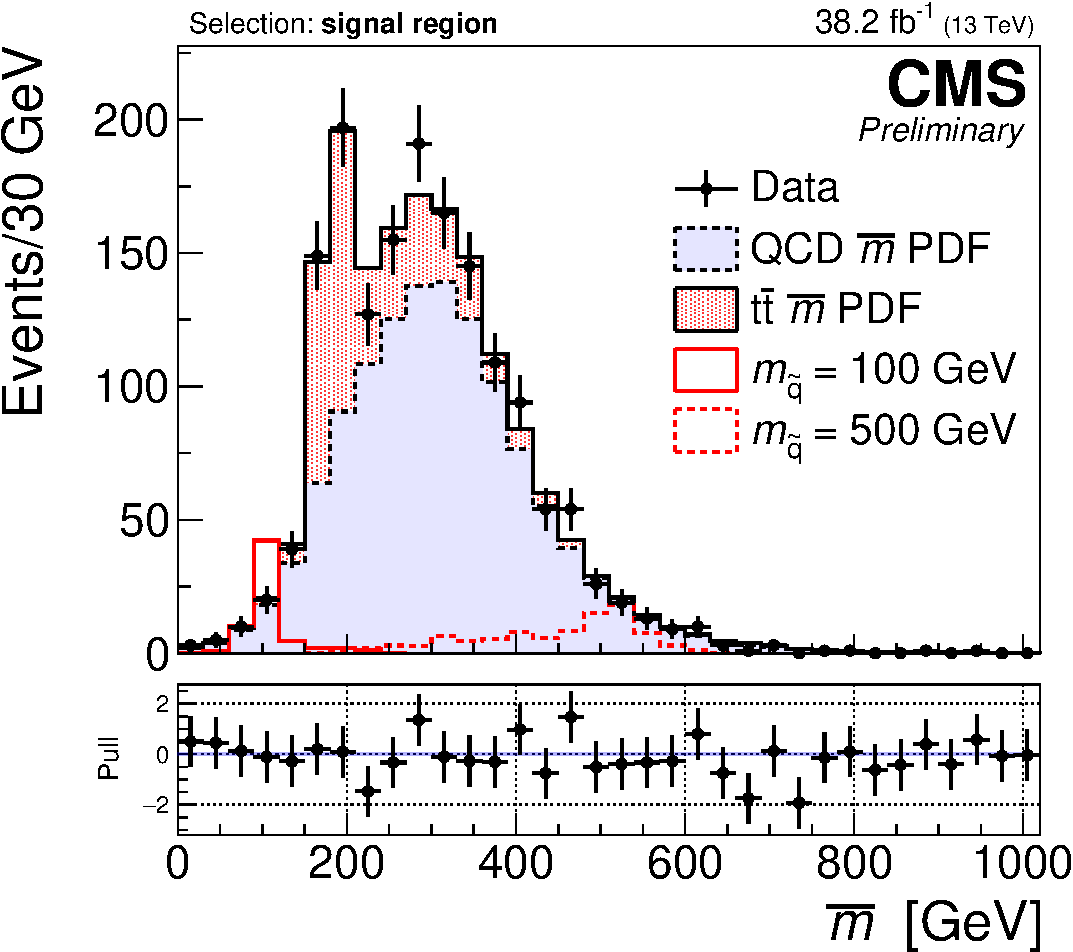
\includegraphics[width=0.48\textwidth]{figures/CMS_search_signal.pdf} \hfill
  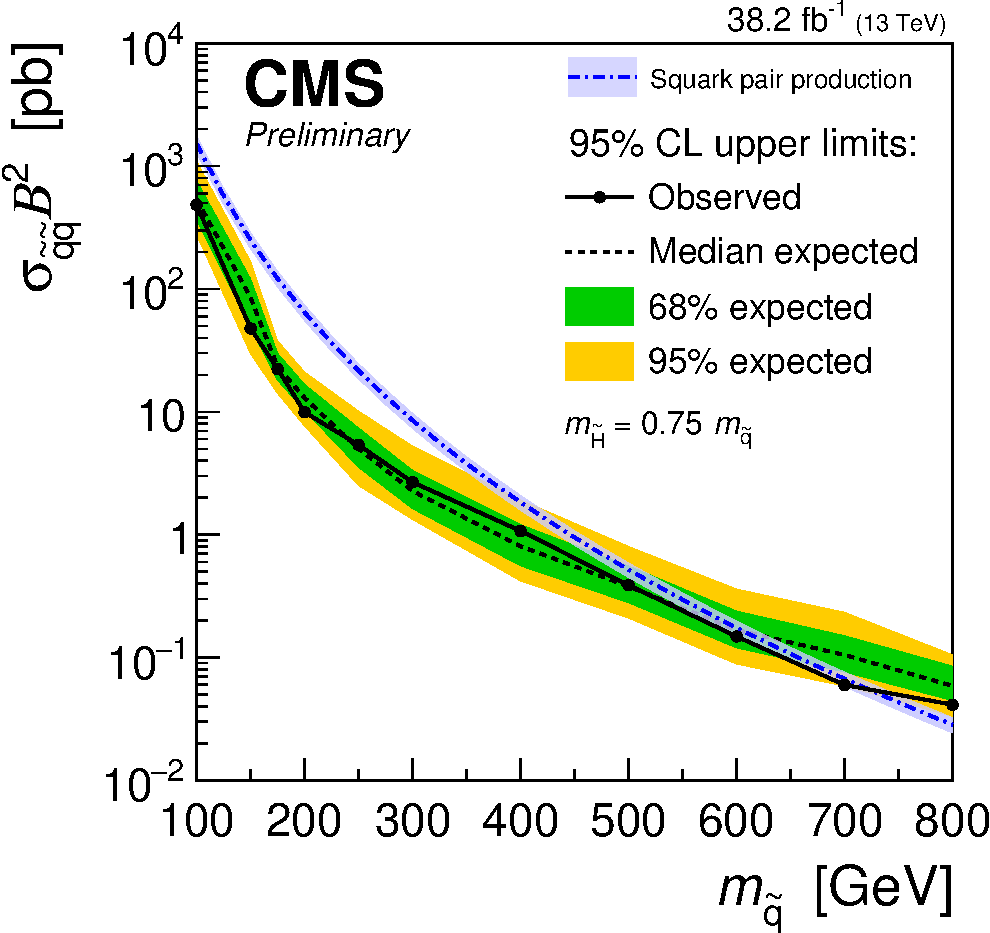
\includegraphics[width=0.47\textwidth]{figures/CMS_search_exlcusion.pdf} 
  \caption{Search for a squark decaying into four quarks (via a Higgsino) performed by CMS \cite{CMS:2018sek}. The plot on the right show the average invariant mass of the fat jets and the exclusion limits.}\label{fig:X_search}
\end{figure}

%% GS helper for auctex
%%% Local Variables:
%%% mode: latex
%%% TeX-master: "notes"
%%% End:

%  LocalWords:  topoclusters BDT DNN aplanarity HEPTopTagger squarks
%  LocalWords:  Supersymmetric trk tunable lego Powheg Kaluza
%  LocalWords:  calorimetry gravitons leptonically dileptonic PUPPI
%  LocalWords:  Sundrum Georgi Machacek Higgsino
